\chapter{Resultados Complementarios del Estudio de Simulación}
\label{aneB_00_00_resultados_simulacion}

Este anexo reúne los resultados del estudio de simulación que no se reportan en el cuerpo del Capítulo~\ref{03_00_00_mezclas_ddp_series_tiempo_funcionales}. Las figuras por origen y por componente corresponden a $M_{\mathrm{ref}} = 10$ en C-1 y C-2 y a $M_{\mathrm{ref}} = 6$ en C-3.

\section{Métricas completas por número de componentes}
\label{aneB_00_01_metricas_por_M}

Las diez métricas del Marco Teórico en el bloque de prueba para cada $M$ del barrido, como promedio sobre las ventanas de ancho $w = 30$, a saber, las cuatro métricas de error para la esperanza del PSBPM-FD, el FAR y el Random Forest, y las seis métricas de intervalo para las tres construcciones de intervalo del PSBPM-FD y para el FAR.

\subsection{Escenario C-1 (GARCH)}
\label{aneB_00_01_02_metricas_garch}

\begin{table}[H]
\centering\footnotesize
\setlength{\tabcolsep}{3pt}
\caption{C-1 (GARCH). Métricas de error en el bloque de prueba por $M$ (promedio sobre las ventanas, $w = 30$).}
\label{tab:aneB_A_C1}
\resizebox{\textwidth}{!}{%
\begin{tabular}{c cccc cccc cccc}
\hline
 & \multicolumn{4}{c}{PSBPM-FD (esperanza)} & \multicolumn{4}{c}{FAR} & \multicolumn{4}{c}{Random Forest} \\
$M$ & MAE & RMSE & $\overline{\mathrm{E}}_{\max}$ & $\mathrm{E}_{\max}^{\mathrm{glob}}$ & MAE & RMSE & $\overline{\mathrm{E}}_{\max}$ & $\mathrm{E}_{\max}^{\mathrm{glob}}$ & MAE & RMSE & $\overline{\mathrm{E}}_{\max}$ & $\mathrm{E}_{\max}^{\mathrm{glob}}$ \\
\hline
$1$ & 0.754 & 0.951 & 1.673 & 3.141 & 0.723 & 0.906 & 1.615 & 2.942 & 0.764 & 0.967 & 1.685 & 3.268 \\
$2$ & 0.739 & 0.923 & 1.644 & 2.949 & 0.723 & 0.906 & 1.615 & 2.942 & 0.753 & 0.943 & 1.668 & 3.111 \\
$3$ & 0.724 & 0.903 & 1.609 & 2.914 & 0.723 & 0.906 & 1.615 & 2.942 & 0.740 & 0.927 & 1.632 & 3.013 \\
$4$ & 0.716 & 0.895 & 1.600 & 2.919 & 0.723 & 0.906 & 1.615 & 2.942 & 0.734 & 0.922 & 1.627 & 3.049 \\
$5$ & 0.714 & 0.893 & 1.592 & 2.893 & 0.723 & 0.906 & 1.615 & 2.942 & 0.733 & 0.921 & 1.623 & 3.020 \\
$6$ & 0.713 & 0.891 & 1.588 & 2.883 & 0.723 & 0.906 & 1.615 & 2.942 & 0.732 & 0.920 & 1.618 & 3.008 \\
$7$ & 0.712 & 0.891 & 1.583 & 2.869 & 0.723 & 0.906 & 1.615 & 2.942 & 0.733 & 0.920 & 1.615 & 3.002 \\
$8$ & 0.712 & 0.890 & 1.581 & 2.859 & 0.723 & 0.906 & 1.615 & 2.942 & 0.733 & 0.920 & 1.612 & 2.985 \\
$9$ & 0.711 & 0.890 & 1.579 & 2.851 & 0.723 & 0.906 & 1.615 & 2.942 & 0.734 & 0.920 & 1.613 & 2.982 \\
$10$ & 0.711 & 0.890 & 1.579 & 2.854 & 0.723 & 0.906 & 1.615 & 2.942 & 0.734 & 0.920 & 1.612 & 2.991 \\
\hline
\end{tabular}}
\end{table}

\begin{table}[H]
\centering\footnotesize
\caption{C-1 (GARCH). Métricas de intervalo en el bloque de prueba por $M$ y construcción de intervalo (promedio sobre las ventanas, $w = 30$).}
\label{tab:aneB_B_C1}
\begin{tabular}{l c cccccc}
\hline
 Banda & $M$ & MPIW & PICP & PICPB & Winkler & $\overline{\mathrm{W}}_{\max}$ & $\mathrm{W}_{\max}^{\mathrm{glob}}$ \\
\hline
PSBPM-FD equi-colas & $1$ & 1.951 & 0.640 & 0.000 & 9.945 & 41.716 & 99.849 \\
PSBPM-FD equi-colas & $2$ & 2.816 & 0.869 & 0.351 & 4.978 & 17.398 & 62.615 \\
PSBPM-FD equi-colas & $3$ & 3.092 & 0.910 & 0.467 & 4.488 & 13.743 & 55.592 \\
PSBPM-FD equi-colas & $4$ & 3.262 & 0.932 & 0.565 & 4.316 & 11.786 & 52.103 \\
PSBPM-FD equi-colas & $5$ & 3.368 & 0.939 & 0.602 & 4.270 & 10.743 & 48.908 \\
PSBPM-FD equi-colas & $6$ & 3.426 & 0.943 & 0.618 & 4.243 & 10.279 & 47.115 \\
PSBPM-FD equi-colas & $7$ & 3.455 & 0.945 & 0.630 & 4.232 & 10.015 & 46.369 \\
PSBPM-FD equi-colas & $8$ & 3.471 & 0.946 & 0.626 & 4.232 & 9.892 & 45.139 \\
PSBPM-FD equi-colas & $9$ & 3.481 & 0.946 & 0.630 & 4.231 & 9.830 & 44.953 \\
PSBPM-FD equi-colas & $10$ & 3.487 & 0.947 & 0.648 & 4.233 & 9.848 & 45.100 \\
\hline
PSBPM-FD simultánea & $1$ & 1.957 & 0.641 & 0.000 & 9.921 & 41.645 & 99.772 \\
PSBPM-FD simultánea & $2$ & 3.700 & 0.953 & 0.642 & 4.438 & 10.316 & 47.483 \\
PSBPM-FD simultánea & $3$ & 4.394 & 0.979 & 0.807 & 4.681 & 7.853 & 33.922 \\
PSBPM-FD simultánea & $4$ & 4.784 & 0.990 & 0.912 & 4.924 & 6.727 & 25.270 \\
PSBPM-FD simultánea & $5$ & 5.015 & 0.993 & 0.940 & 5.110 & 6.564 & 21.591 \\
PSBPM-FD simultánea & $6$ & 5.116 & 0.994 & 0.952 & 5.194 & 6.449 & 19.148 \\
PSBPM-FD simultánea & $7$ & 5.190 & 0.995 & 0.958 & 5.261 & 6.476 & 18.141 \\
PSBPM-FD simultánea & $8$ & 5.227 & 0.995 & 0.963 & 5.295 & 6.456 & 17.180 \\
PSBPM-FD simultánea & $9$ & 5.253 & 0.995 & 0.966 & 5.321 & 6.494 & 17.043 \\
PSBPM-FD simultánea & $10$ & 5.262 & 0.995 & 0.966 & 5.327 & 6.473 & 16.809 \\
\hline
PSBPM-FD HDR & $1$ & 1.951 & 0.640 & 0.000 & 9.934 & 41.676 & 99.618 \\
PSBPM-FD HDR & $2$ & 2.819 & 0.872 & 0.365 & 4.936 & 17.004 & 61.792 \\
PSBPM-FD HDR & $3$ & 3.096 & 0.911 & 0.481 & 4.463 & 13.497 & 55.184 \\
PSBPM-FD HDR & $4$ & 3.268 & 0.932 & 0.566 & 4.303 & 11.600 & 52.307 \\
PSBPM-FD HDR & $5$ & 3.374 & 0.942 & 0.617 & 4.263 & 10.512 & 48.065 \\
PSBPM-FD HDR & $6$ & 3.432 & 0.945 & 0.636 & 4.242 & 10.136 & 47.008 \\
PSBPM-FD HDR & $7$ & 3.462 & 0.947 & 0.647 & 4.232 & 9.842 & 45.841 \\
PSBPM-FD HDR & $8$ & 3.478 & 0.948 & 0.663 & 4.231 & 9.726 & 44.701 \\
PSBPM-FD HDR & $9$ & 3.488 & 0.948 & 0.669 & 4.230 & 9.607 & 44.055 \\
PSBPM-FD HDR & $10$ & 3.493 & 0.948 & 0.658 & 4.231 & 9.598 & 44.142 \\
\hline
FAR & $1$ & 3.423 & 0.940 & 0.625 & 4.352 & 10.404 & 51.188 \\
FAR & $2$ & 3.423 & 0.940 & 0.625 & 4.352 & 10.404 & 51.188 \\
FAR & $3$ & 3.423 & 0.940 & 0.625 & 4.352 & 10.404 & 51.188 \\
FAR & $4$ & 3.423 & 0.940 & 0.625 & 4.352 & 10.404 & 51.188 \\
FAR & $5$ & 3.423 & 0.940 & 0.625 & 4.352 & 10.404 & 51.188 \\
FAR & $6$ & 3.423 & 0.940 & 0.625 & 4.352 & 10.404 & 51.188 \\
FAR & $7$ & 3.423 & 0.940 & 0.625 & 4.352 & 10.404 & 51.188 \\
FAR & $8$ & 3.423 & 0.940 & 0.625 & 4.352 & 10.404 & 51.188 \\
FAR & $9$ & 3.423 & 0.940 & 0.625 & 4.352 & 10.404 & 51.188 \\
FAR & $10$ & 3.423 & 0.940 & 0.625 & 4.352 & 10.404 & 51.188 \\
\hline
\end{tabular}
\end{table}

\subsection{Escenario C-2 (TAR)}
\label{aneB_00_01_01_metricas_tar}

\begin{table}[H]
\centering\footnotesize
\setlength{\tabcolsep}{3pt}
\caption{C-2 (TAR). Métricas de error en el bloque de prueba por $M$ (promedio sobre las ventanas, $w = 30$).}
\label{tab:aneB_A_C2}
\resizebox{\textwidth}{!}{%
\begin{tabular}{c cccc cccc cccc}
\hline
 & \multicolumn{4}{c}{PSBPM-FD (esperanza)} & \multicolumn{4}{c}{FAR} & \multicolumn{4}{c}{Random Forest} \\
$M$ & MAE & RMSE & $\overline{\mathrm{E}}_{\max}$ & $\mathrm{E}_{\max}^{\mathrm{glob}}$ & MAE & RMSE & $\overline{\mathrm{E}}_{\max}$ & $\mathrm{E}_{\max}^{\mathrm{glob}}$ & MAE & RMSE & $\overline{\mathrm{E}}_{\max}$ & $\mathrm{E}_{\max}^{\mathrm{glob}}$ \\
\hline
$1$ & 0.714 & 0.906 & 1.634 & 3.073 & 0.770 & 0.980 & 1.737 & 3.343 & 0.710 & 0.906 & 1.625 & 3.101 \\
$2$ & 0.673 & 0.854 & 1.564 & 2.922 & 0.770 & 0.980 & 1.737 & 3.343 & 0.658 & 0.843 & 1.522 & 2.982 \\
$3$ & 0.635 & 0.808 & 1.472 & 2.800 & 0.770 & 0.980 & 1.737 & 3.343 & 0.617 & 0.793 & 1.428 & 2.867 \\
$4$ & 0.612 & 0.783 & 1.410 & 2.796 & 0.770 & 0.980 & 1.737 & 3.343 & 0.591 & 0.767 & 1.361 & 2.786 \\
$5$ & 0.610 & 0.781 & 1.407 & 2.769 & 0.770 & 0.980 & 1.737 & 3.343 & 0.591 & 0.766 & 1.363 & 2.748 \\
$6$ & 0.609 & 0.779 & 1.401 & 2.770 & 0.770 & 0.980 & 1.737 & 3.343 & 0.592 & 0.766 & 1.363 & 2.784 \\
$7$ & 0.609 & 0.778 & 1.398 & 2.766 & 0.770 & 0.980 & 1.737 & 3.343 & 0.592 & 0.766 & 1.362 & 2.773 \\
$8$ & 0.609 & 0.777 & 1.396 & 2.758 & 0.770 & 0.980 & 1.737 & 3.343 & 0.592 & 0.766 & 1.361 & 2.756 \\
$9$ & 0.609 & 0.777 & 1.395 & 2.749 & 0.770 & 0.980 & 1.737 & 3.343 & 0.591 & 0.766 & 1.360 & 2.743 \\
$10$ & 0.609 & 0.777 & 1.393 & 2.750 & 0.770 & 0.980 & 1.737 & 3.343 & 0.591 & 0.766 & 1.360 & 2.748 \\
\hline
\end{tabular}}
\end{table}

\begin{table}[H]
\centering\footnotesize
\caption{C-2 (TAR). Métricas de intervalo en el bloque de prueba por $M$ y construcción de intervalo (promedio sobre las ventanas, $w = 30$).}
\label{tab:aneB_B_C2}
\begin{tabular}{l c cccccc}
\hline
 Banda & $M$ & MPIW & PICP & PICPB & Winkler & $\overline{\mathrm{W}}_{\max}$ & $\mathrm{W}_{\max}^{\mathrm{glob}}$ \\
\hline
PSBPM-FD equi-colas & $1$ & 1.764 & 0.541 & 0.000 & 11.953 & 45.955 & 110.153 \\
PSBPM-FD equi-colas & $2$ & 2.787 & 0.817 & 0.154 & 5.693 & 23.434 & 68.181 \\
PSBPM-FD equi-colas & $3$ & 3.135 & 0.891 & 0.252 & 4.614 & 16.974 & 56.964 \\
PSBPM-FD equi-colas & $4$ & 3.351 & 0.945 & 0.503 & 3.968 & 10.283 & 45.603 \\
PSBPM-FD equi-colas & $5$ & 3.450 & 0.957 & 0.572 & 3.913 & 8.928 & 40.835 \\
PSBPM-FD equi-colas & $6$ & 3.511 & 0.964 & 0.652 & 3.900 & 8.201 & 40.471 \\
PSBPM-FD equi-colas & $7$ & 3.542 & 0.967 & 0.663 & 3.902 & 7.961 & 39.779 \\
PSBPM-FD equi-colas & $8$ & 3.560 & 0.968 & 0.685 & 3.907 & 7.791 & 37.839 \\
PSBPM-FD equi-colas & $9$ & 3.570 & 0.968 & 0.678 & 3.909 & 7.743 & 37.752 \\
PSBPM-FD equi-colas & $10$ & 3.576 & 0.969 & 0.691 & 3.907 & 7.604 & 37.533 \\
\hline
PSBPM-FD simultánea & $1$ & 2.009 & 0.604 & 0.000 & 10.735 & 42.834 & 109.617 \\
PSBPM-FD simultánea & $2$ & 6.083 & 0.968 & 0.778 & 6.538 & 11.939 & 43.678 \\
PSBPM-FD simultánea & $3$ & 7.787 & 0.992 & 0.893 & 7.907 & 12.119 & 33.362 \\
PSBPM-FD simultánea & $4$ & 6.709 & 0.998 & 0.971 & 6.731 & 9.005 & 21.686 \\
PSBPM-FD simultánea & $5$ & 6.552 & 0.999 & 0.979 & 6.572 & 8.548 & 19.294 \\
PSBPM-FD simultánea & $6$ & 6.310 & 0.999 & 0.983 & 6.325 & 8.008 & 16.702 \\
PSBPM-FD simultánea & $7$ & 6.398 & 0.999 & 0.983 & 6.414 & 8.064 & 16.556 \\
PSBPM-FD simultánea & $8$ & 6.344 & 0.999 & 0.986 & 6.358 & 7.935 & 15.688 \\
PSBPM-FD simultánea & $9$ & 6.355 & 0.999 & 0.983 & 6.368 & 7.921 & 15.599 \\
PSBPM-FD simultánea & $10$ & 6.350 & 0.999 & 0.986 & 6.363 & 7.898 & 15.492 \\
\hline
PSBPM-FD HDR & $1$ & 1.460 & 0.493 & 0.000 & 12.085 & 45.327 & 110.408 \\
PSBPM-FD HDR & $2$ & 2.557 & 0.813 & 0.188 & 5.286 & 21.219 & 68.502 \\
PSBPM-FD HDR & $3$ & 2.970 & 0.899 & 0.286 & 4.314 & 15.155 & 56.477 \\
PSBPM-FD HDR & $4$ & 3.234 & 0.955 & 0.606 & 3.747 & 8.748 & 44.656 \\
PSBPM-FD HDR & $5$ & 3.349 & 0.965 & 0.673 & 3.750 & 7.807 & 40.742 \\
PSBPM-FD HDR & $6$ & 3.419 & 0.971 & 0.723 & 3.765 & 7.376 & 40.151 \\
PSBPM-FD HDR & $7$ & 3.453 & 0.974 & 0.741 & 3.775 & 7.143 & 39.764 \\
PSBPM-FD HDR & $8$ & 3.474 & 0.974 & 0.760 & 3.783 & 7.067 & 38.241 \\
PSBPM-FD HDR & $9$ & 3.486 & 0.975 & 0.761 & 3.790 & 7.016 & 37.498 \\
PSBPM-FD HDR & $10$ & 3.492 & 0.975 & 0.765 & 3.793 & 6.973 & 37.556 \\
\hline
FAR & $1$ & 3.977 & 0.952 & 0.702 & 4.863 & 10.998 & 59.076 \\
FAR & $2$ & 3.977 & 0.952 & 0.702 & 4.863 & 10.998 & 59.076 \\
FAR & $3$ & 3.977 & 0.952 & 0.702 & 4.863 & 10.998 & 59.076 \\
FAR & $4$ & 3.977 & 0.952 & 0.702 & 4.863 & 10.998 & 59.076 \\
FAR & $5$ & 3.977 & 0.952 & 0.702 & 4.863 & 10.998 & 59.076 \\
FAR & $6$ & 3.977 & 0.952 & 0.702 & 4.863 & 10.998 & 59.076 \\
FAR & $7$ & 3.977 & 0.952 & 0.702 & 4.863 & 10.998 & 59.076 \\
FAR & $8$ & 3.977 & 0.952 & 0.702 & 4.863 & 10.998 & 59.076 \\
FAR & $9$ & 3.977 & 0.952 & 0.702 & 4.863 & 10.998 & 59.076 \\
FAR & $10$ & 3.977 & 0.952 & 0.702 & 4.863 & 10.998 & 59.076 \\
\hline
\end{tabular}
\end{table}

\subsection{Escenario C-3 (multimodalidad)}
\label{aneB_00_01_03_metricas_multimodal}

\begin{table}[H]
\centering\footnotesize
\setlength{\tabcolsep}{3pt}
\caption{C-3 (multimodalidad). Métricas de error en el bloque de prueba por $M$ (promedio sobre las ventanas, $w = 30$).}
\label{tab:aneB_A_C3}
\resizebox{\textwidth}{!}{%
\begin{tabular}{c cccc cccc cccc}
\hline
 & \multicolumn{4}{c}{PSBPM-FD (esperanza)} & \multicolumn{4}{c}{FAR} & \multicolumn{4}{c}{Random Forest} \\
$M$ & MAE & RMSE & $\overline{\mathrm{E}}_{\max}$ & $\mathrm{E}_{\max}^{\mathrm{glob}}$ & MAE & RMSE & $\overline{\mathrm{E}}_{\max}$ & $\mathrm{E}_{\max}^{\mathrm{glob}}$ & MAE & RMSE & $\overline{\mathrm{E}}_{\max}$ & $\mathrm{E}_{\max}^{\mathrm{glob}}$ \\
\hline
$3$ & 0.694 & 0.870 & 1.612 & 3.038 & 0.700 & 0.880 & 1.635 & 2.951 & 0.699 & 0.878 & 1.632 & 3.071 \\
$4$ & 0.689 & 0.866 & 1.602 & 3.001 & 0.700 & 0.880 & 1.635 & 2.951 & 0.699 & 0.877 & 1.636 & 3.057 \\
$5$ & 0.684 & 0.860 & 1.589 & 2.954 & 0.700 & 0.880 & 1.635 & 2.951 & 0.693 & 0.870 & 1.619 & 2.967 \\
$6$ & 0.689 & 0.866 & 1.598 & 2.968 & 0.700 & 0.880 & 1.635 & 2.951 & 0.700 & 0.877 & 1.630 & 2.984 \\
\hline
\end{tabular}}
\end{table}

\begin{table}[H]
\centering\footnotesize
\caption{C-3 (multimodalidad). Métricas de intervalo en el bloque de prueba por $M$ y construcción de intervalo (promedio sobre las ventanas, $w = 30$).}
\label{tab:aneB_B_C3}
\begin{tabular}{l c cccccc}
\hline
 Banda & $M$ & MPIW & PICP & PICPB & Winkler & $\overline{\mathrm{W}}_{\max}$ & $\mathrm{W}_{\max}^{\mathrm{glob}}$ \\
\hline
PSBPM-FD equi-colas & $3$ & 2.978 & 0.908 & 0.420 & 4.315 & 14.396 & 59.891 \\
PSBPM-FD equi-colas & $4$ & 3.162 & 0.931 & 0.531 & 4.150 & 12.207 & 54.741 \\
PSBPM-FD equi-colas & $5$ & 3.263 & 0.943 & 0.569 & 4.082 & 11.104 & 52.207 \\
PSBPM-FD equi-colas & $6$ & 3.326 & 0.944 & 0.580 & 4.106 & 10.728 & 52.299 \\
\hline
PSBPM-FD simultánea & $3$ & 4.163 & 0.980 & 0.779 & 4.415 & 7.687 & 40.463 \\
PSBPM-FD simultánea & $4$ & 4.595 & 0.991 & 0.901 & 4.710 & 6.475 & 29.982 \\
PSBPM-FD simultánea & $5$ & 4.800 & 0.993 & 0.923 & 4.888 & 6.335 & 25.380 \\
PSBPM-FD simultánea & $6$ & 4.926 & 0.995 & 0.930 & 4.991 & 6.242 & 23.983 \\
\hline
PSBPM-FD HDR & $3$ & 2.982 & 0.910 & 0.443 & 4.313 & 14.333 & 61.098 \\
PSBPM-FD HDR & $4$ & 3.168 & 0.931 & 0.519 & 4.156 & 12.237 & 55.550 \\
PSBPM-FD HDR & $5$ & 3.269 & 0.942 & 0.558 & 4.094 & 11.138 & 53.564 \\
PSBPM-FD HDR & $6$ & 3.333 & 0.945 & 0.589 & 4.111 & 10.796 & 53.141 \\
\hline
FAR & $3$ & 3.283 & 0.937 & 0.563 & 4.230 & 11.835 & 54.523 \\
FAR & $4$ & 3.283 & 0.937 & 0.563 & 4.230 & 11.835 & 54.523 \\
FAR & $5$ & 3.283 & 0.937 & 0.563 & 4.230 & 11.835 & 54.523 \\
FAR & $6$ & 3.283 & 0.937 & 0.563 & 4.230 & 11.835 & 54.523 \\
\hline
\end{tabular}
\end{table}

\section{Sensibilidad al ancho de la ventana}
\label{aneB_00_02_sensibilidad_ventana}

Métricas de error y de intervalo sobre la ventana móvil con $w = 20$ (izquierda) y $w = 40$ (derecha) para todos los $M$ del barrido. El cuerpo reporta $w = 30$.

\begin{figure}[H]
\centering
\begin{minipage}{0.49\textwidth}\centering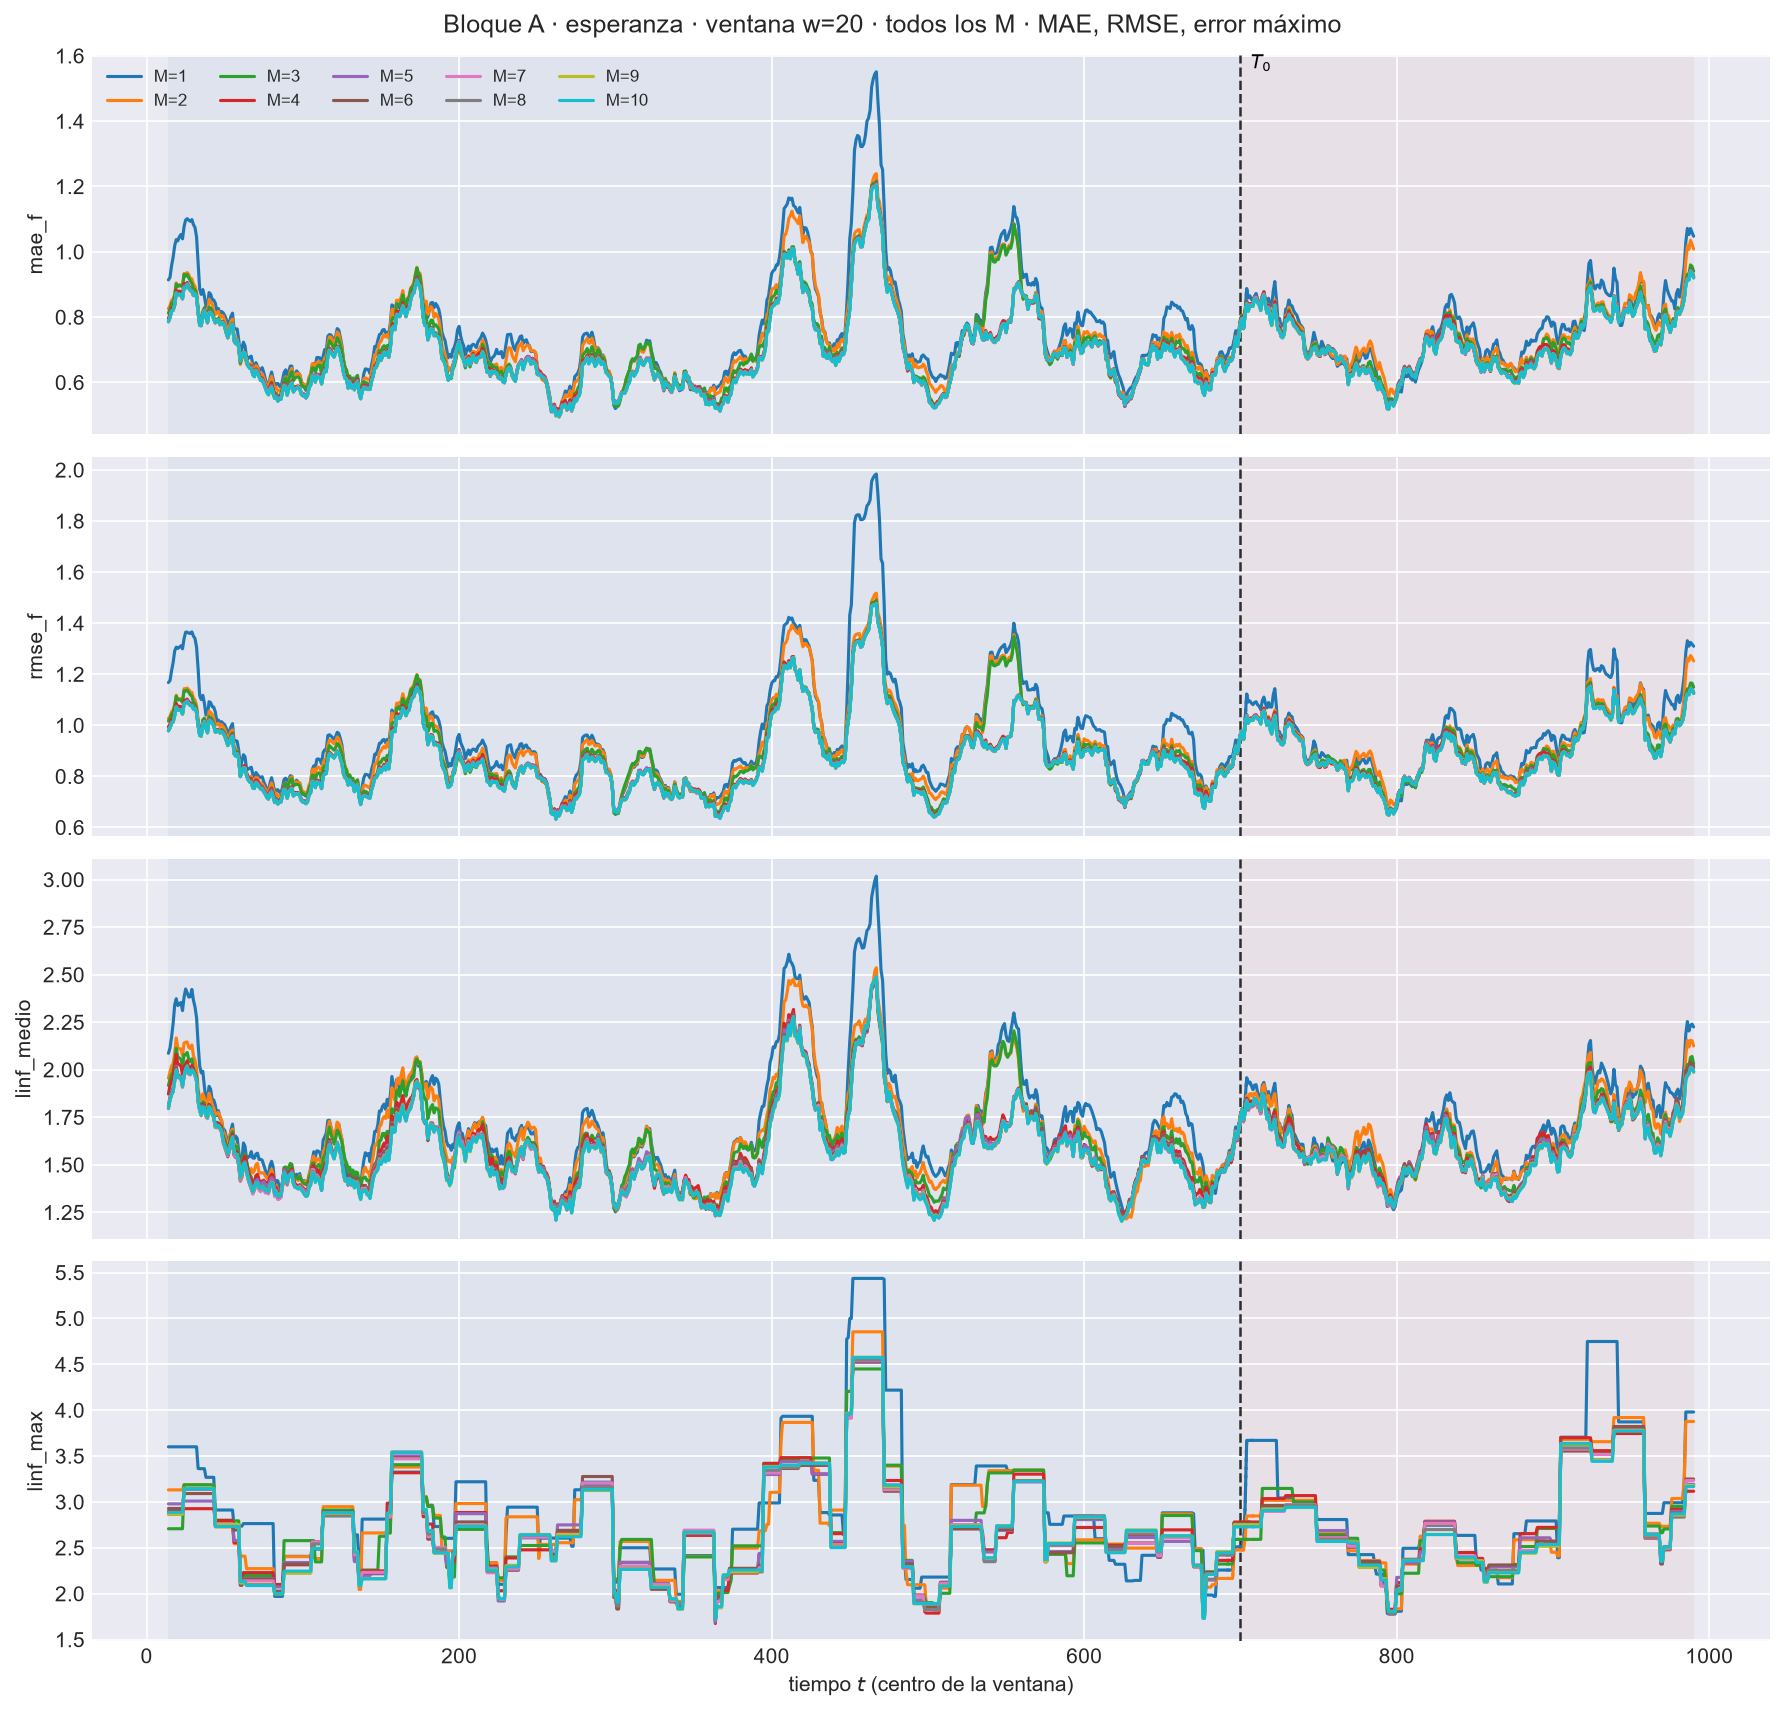
\includegraphics[width=\textwidth]{IMG/aneB_00/aneB_00_bloqueA_w20_C1.png}\end{minipage}\hfill
\begin{minipage}{0.49\textwidth}\centering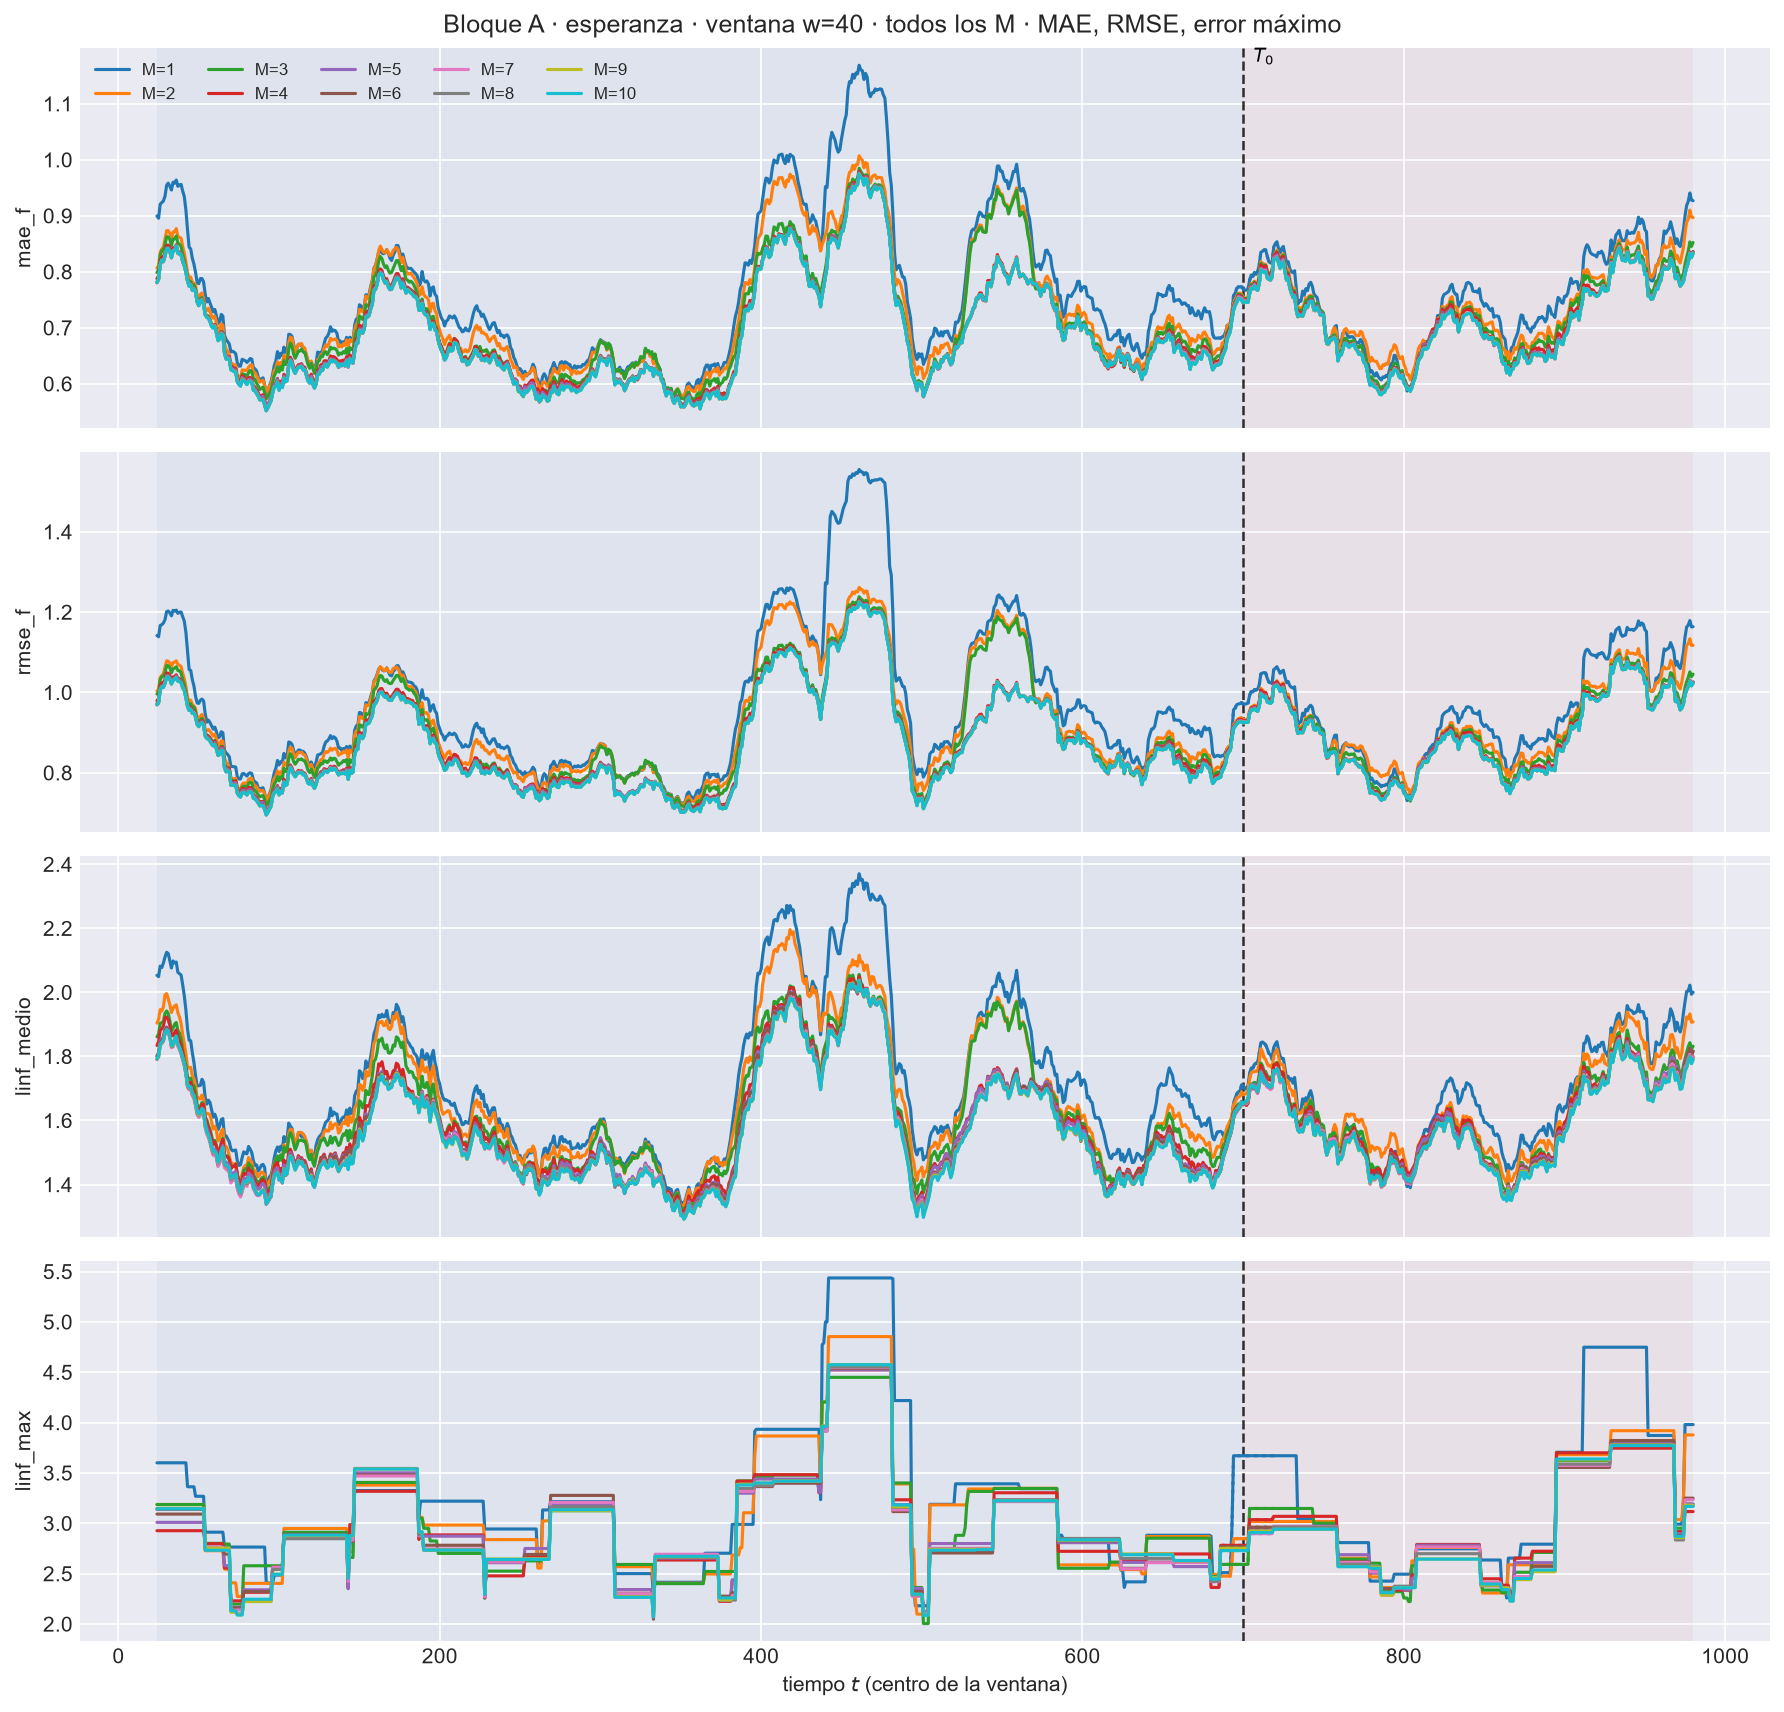
\includegraphics[width=\textwidth]{IMG/aneB_00/aneB_00_bloqueA_w40_C1.png}\end{minipage}
\caption{C-1 (GARCH). Métricas de error sobre la ventana móvil con $w = 20$ (izquierda) y $w = 40$ (derecha).}
\label{fig:aneB_ancho_A_C1}
\end{figure}

\begin{figure}[H]
\centering
\begin{minipage}{0.49\textwidth}\centering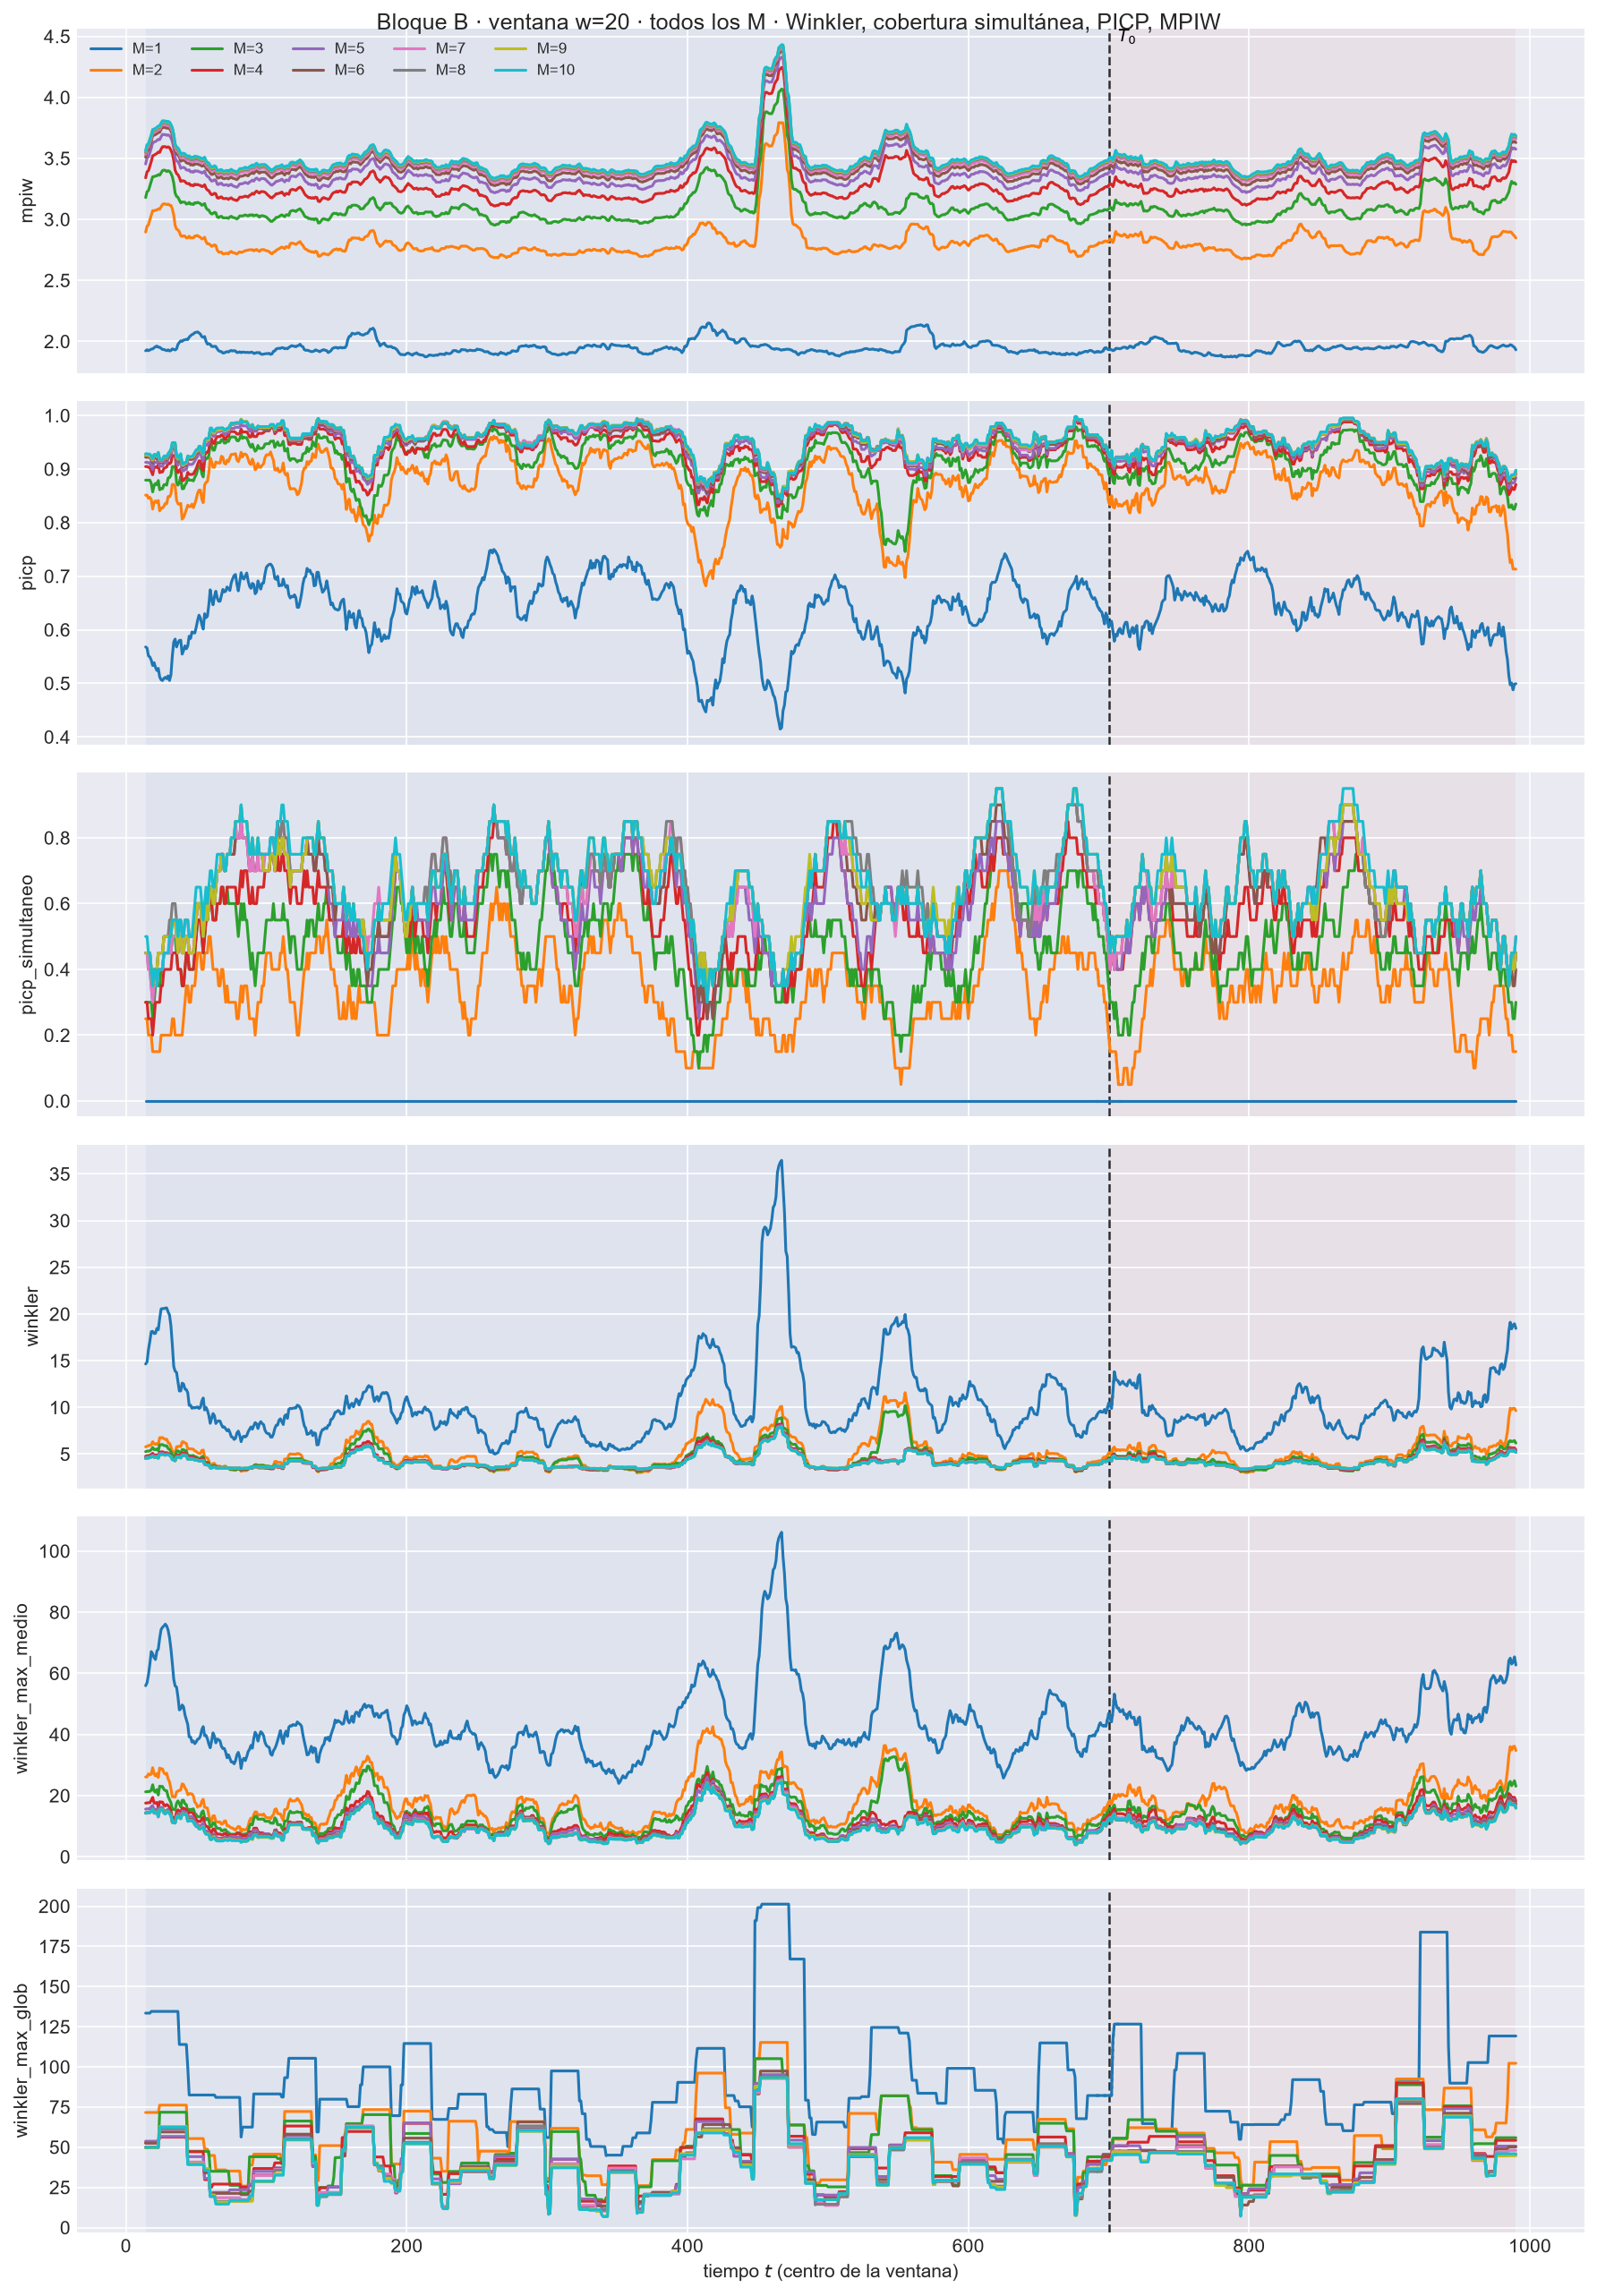
\includegraphics[width=\textwidth]{IMG/aneB_00/aneB_00_bloqueB_w20_C1.png}\end{minipage}\hfill
\begin{minipage}{0.49\textwidth}\centering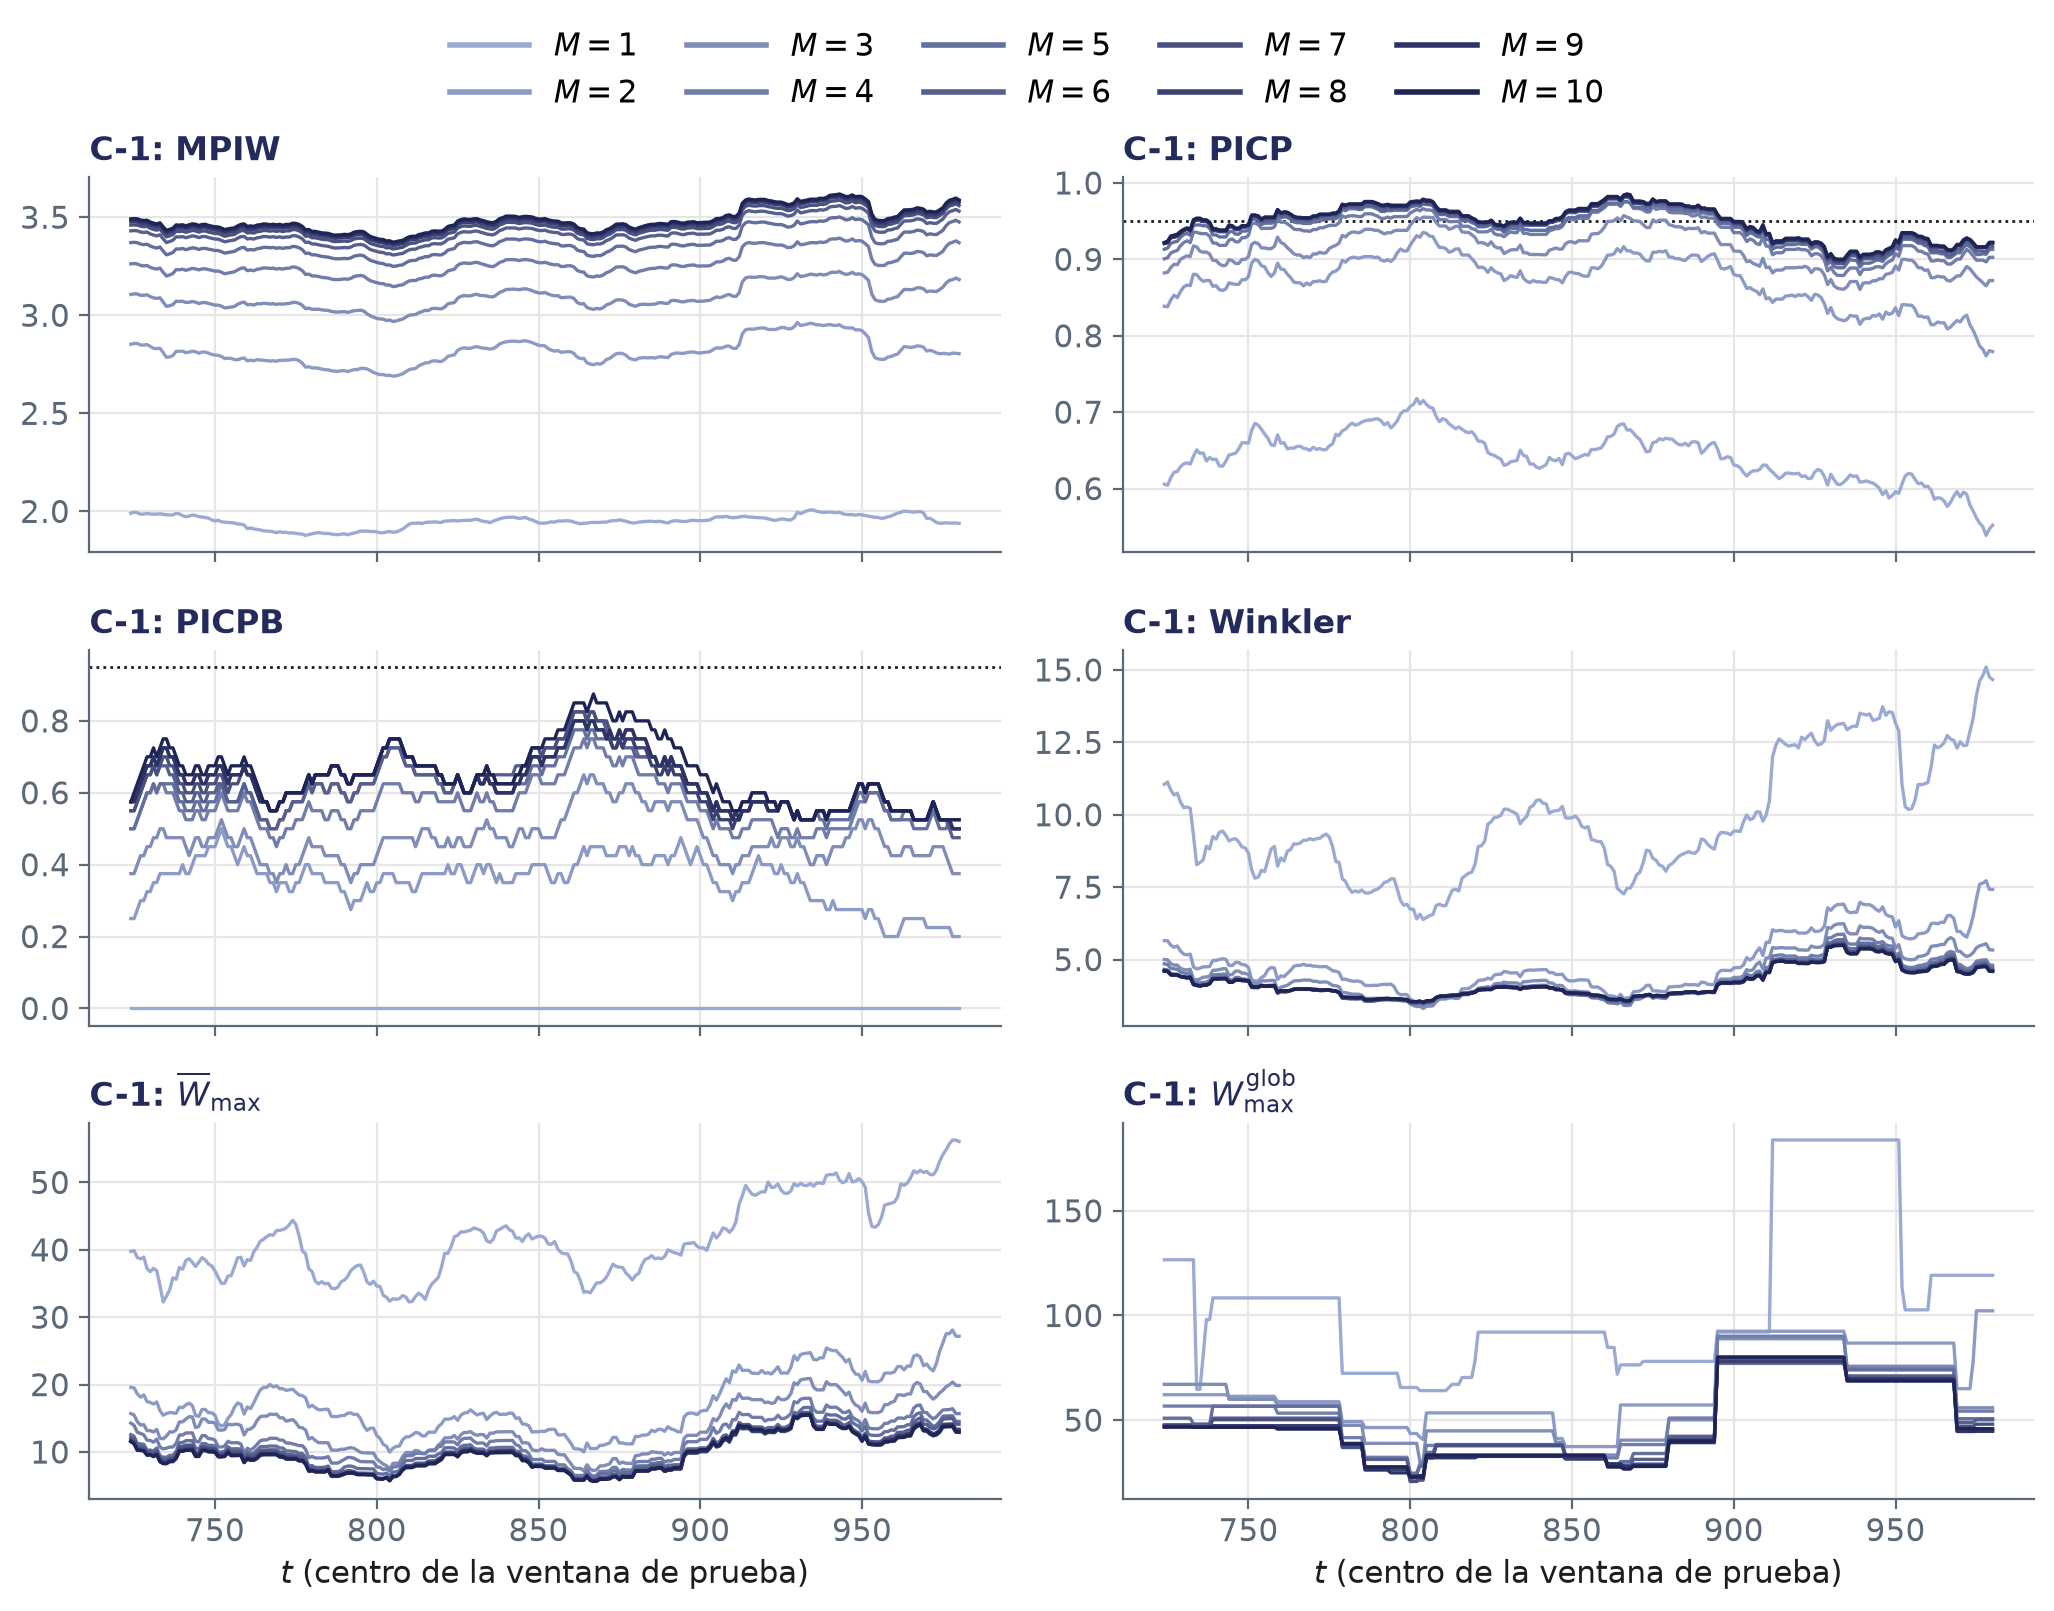
\includegraphics[width=\textwidth]{IMG/aneB_00/aneB_00_bloqueB_w40_C1.png}\end{minipage}
\caption{C-1 (GARCH). Métricas de intervalo sobre la ventana móvil con $w = 20$ (izquierda) y $w = 40$ (derecha).}
\label{fig:aneB_ancho_B_C1}
\end{figure}

\begin{figure}[H]
\centering
\begin{minipage}{0.49\textwidth}\centering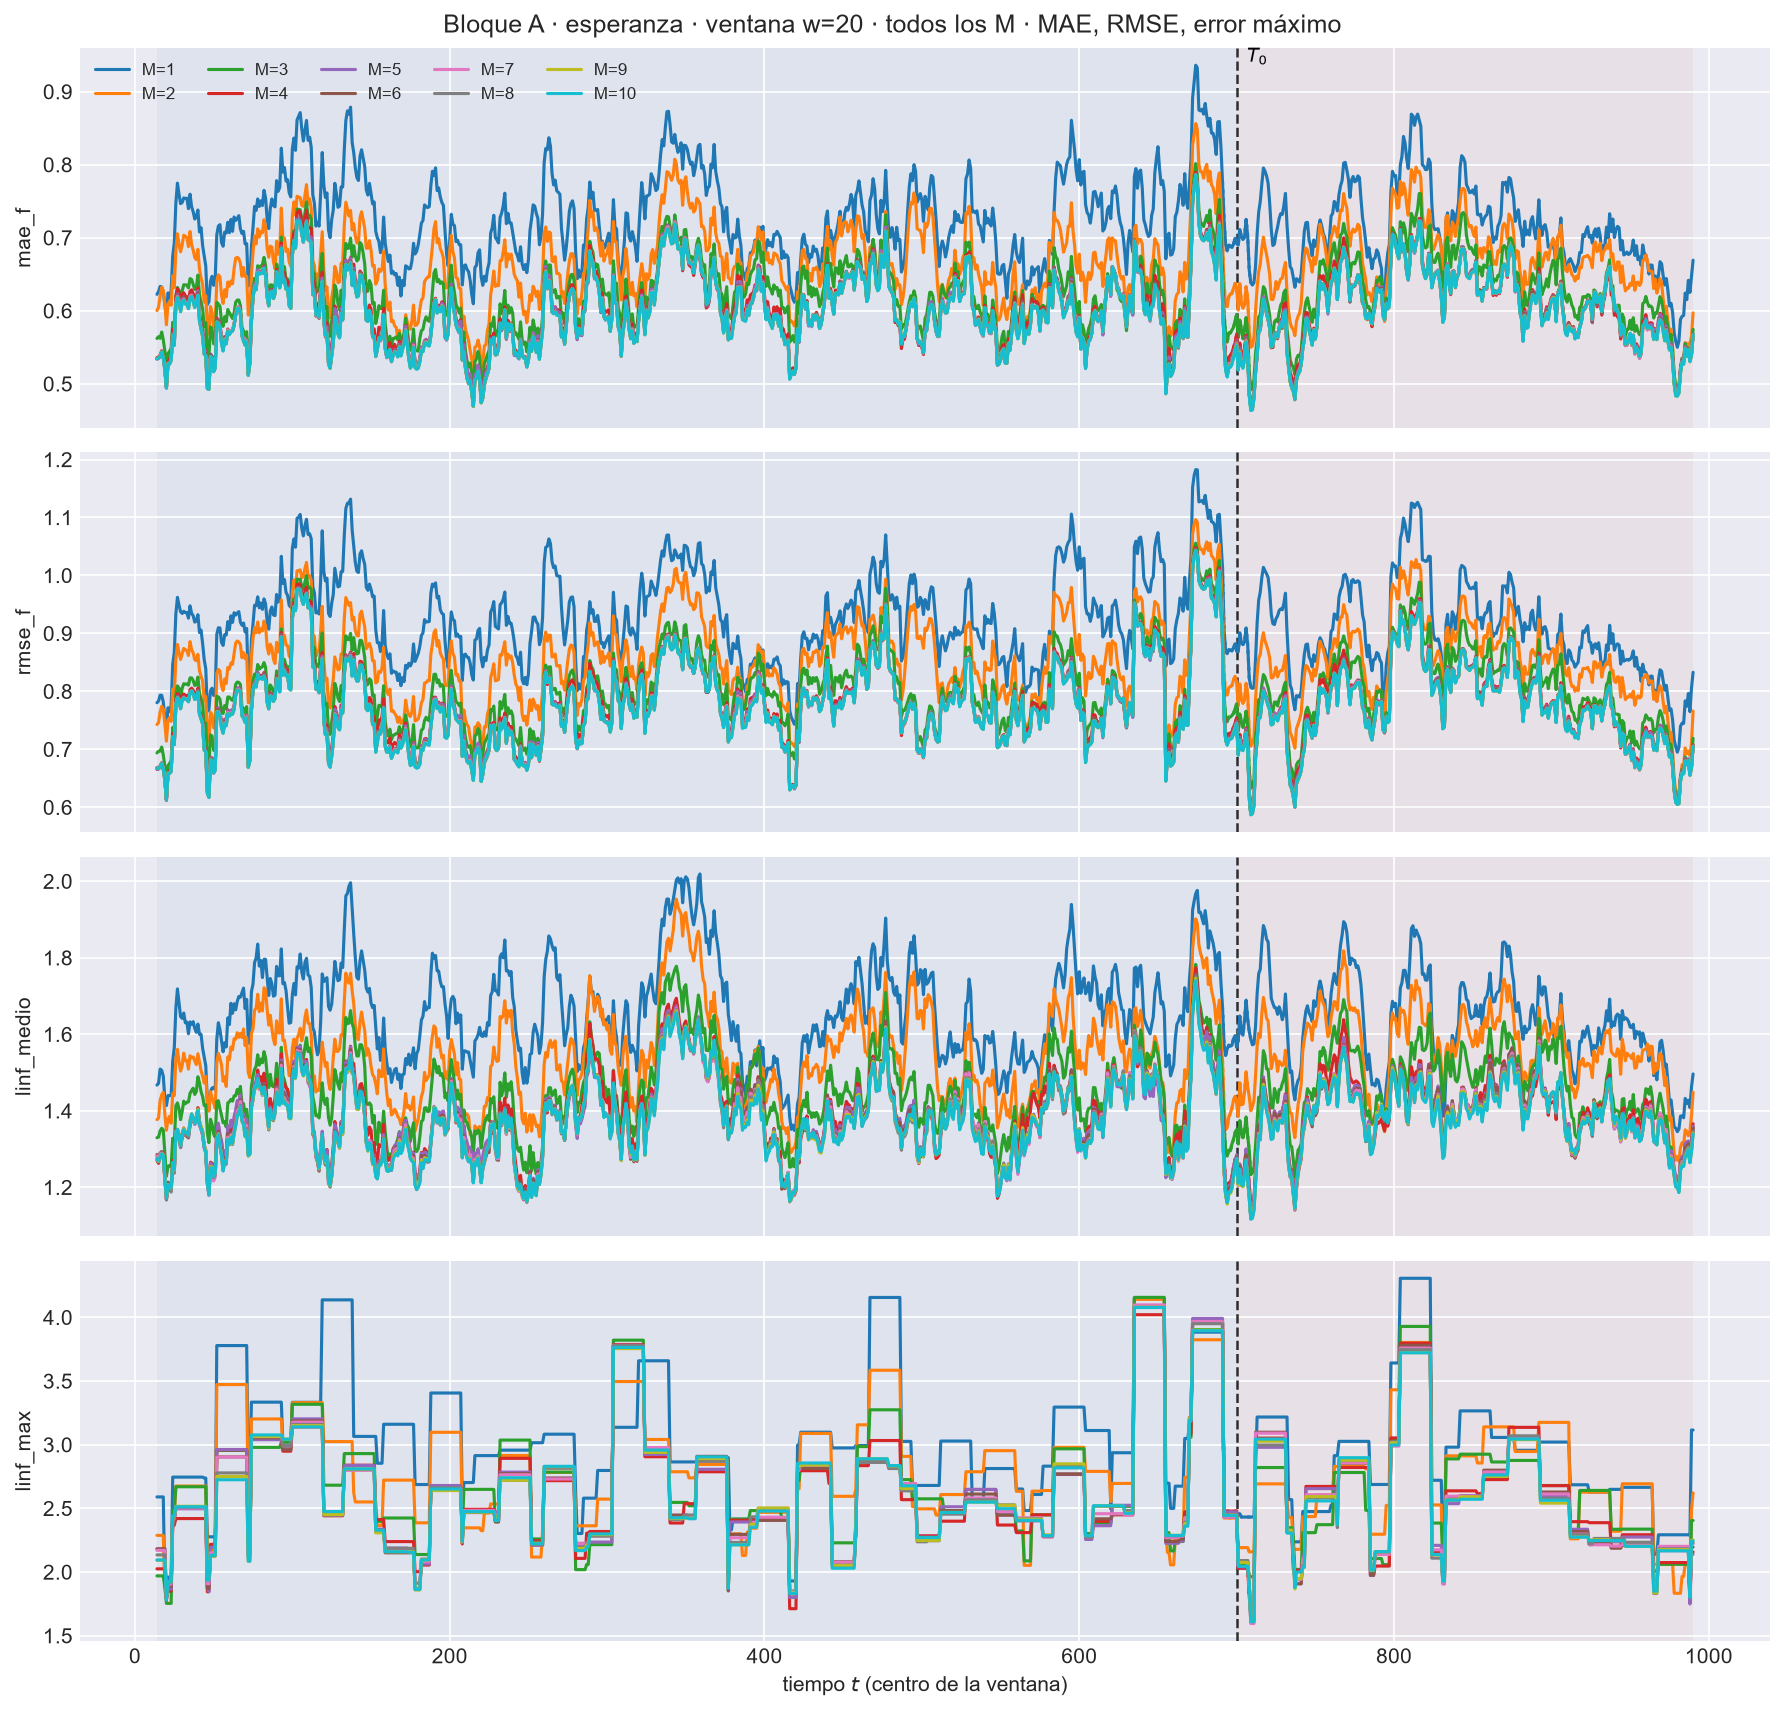
\includegraphics[width=\textwidth]{IMG/aneB_00/aneB_00_bloqueA_w20_C2.png}\end{minipage}\hfill
\begin{minipage}{0.49\textwidth}\centering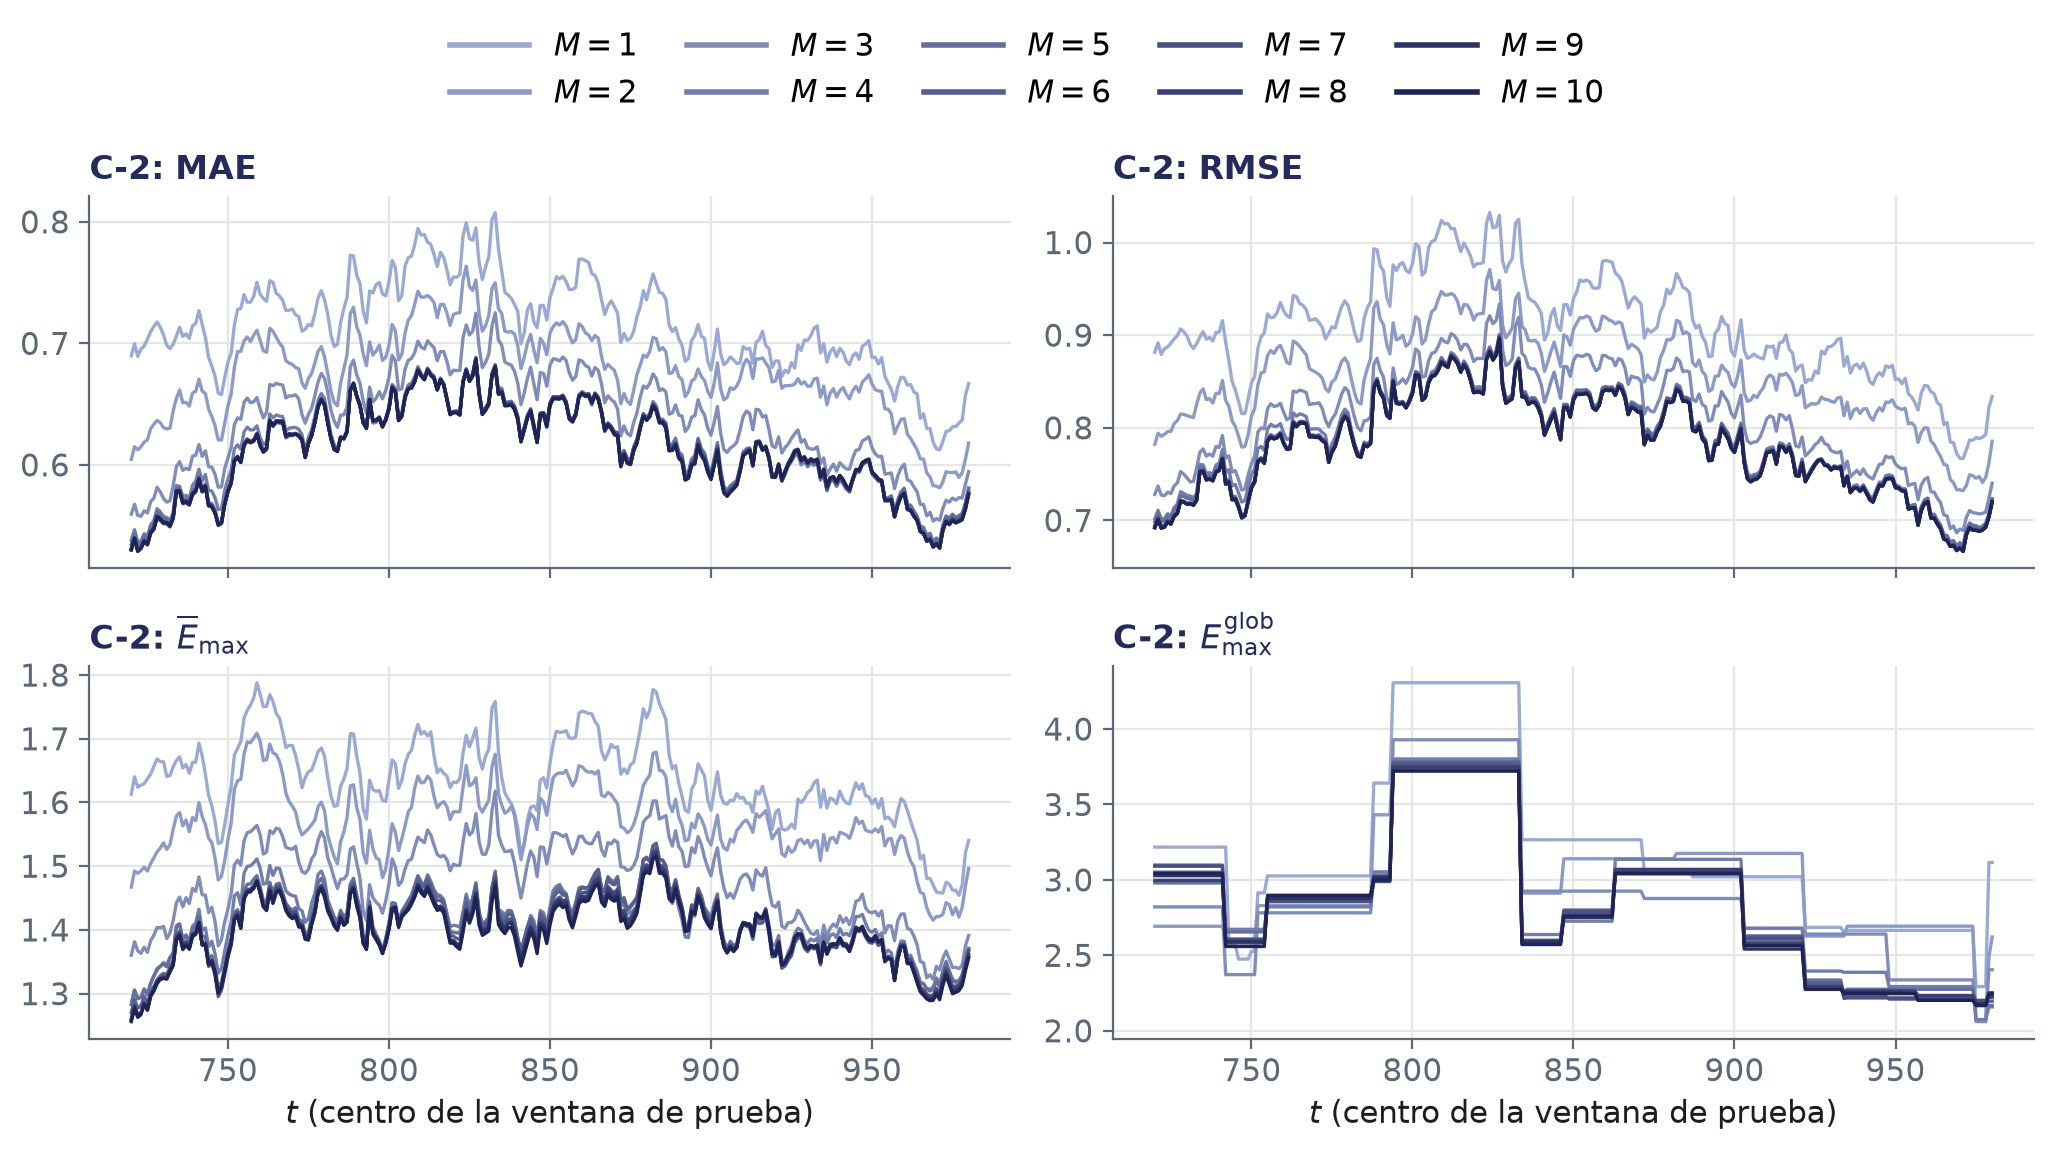
\includegraphics[width=\textwidth]{IMG/aneB_00/aneB_00_bloqueA_w40_C2.png}\end{minipage}
\caption{C-2 (TAR). Métricas de error sobre la ventana móvil con $w = 20$ (izquierda) y $w = 40$ (derecha).}
\label{fig:aneB_ancho_A_C2}
\end{figure}

\begin{figure}[H]
\centering
\begin{minipage}{0.49\textwidth}\centering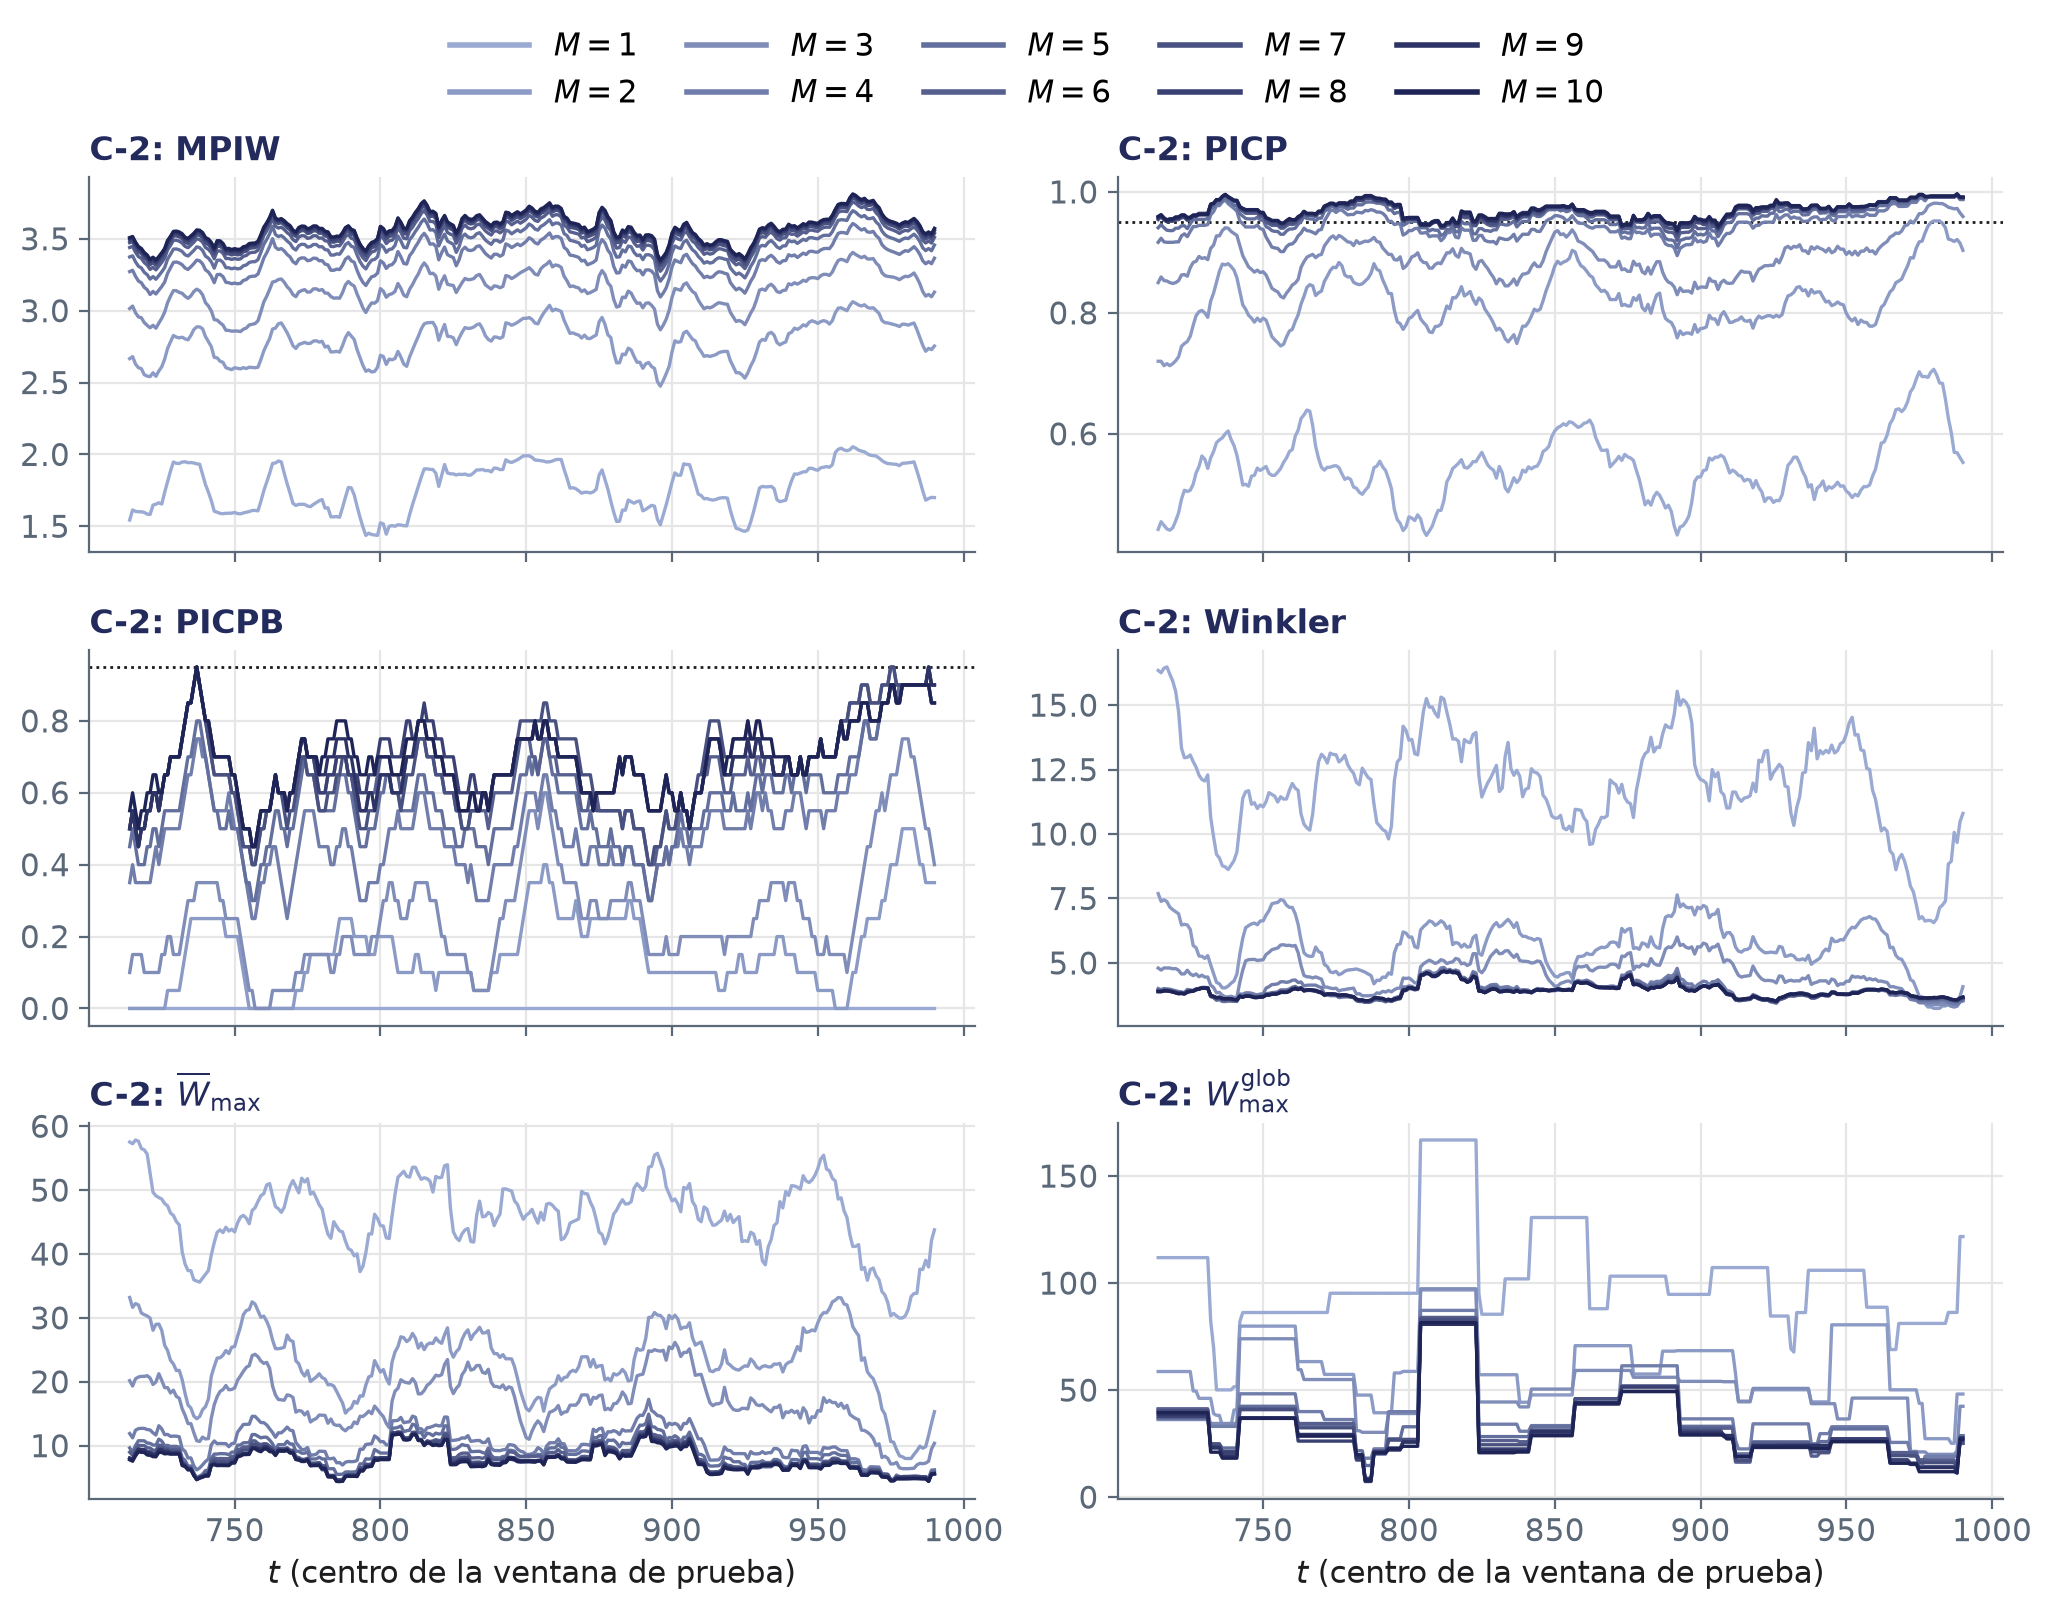
\includegraphics[width=\textwidth]{IMG/aneB_00/aneB_00_bloqueB_w20_C2.png}\end{minipage}\hfill
\begin{minipage}{0.49\textwidth}\centering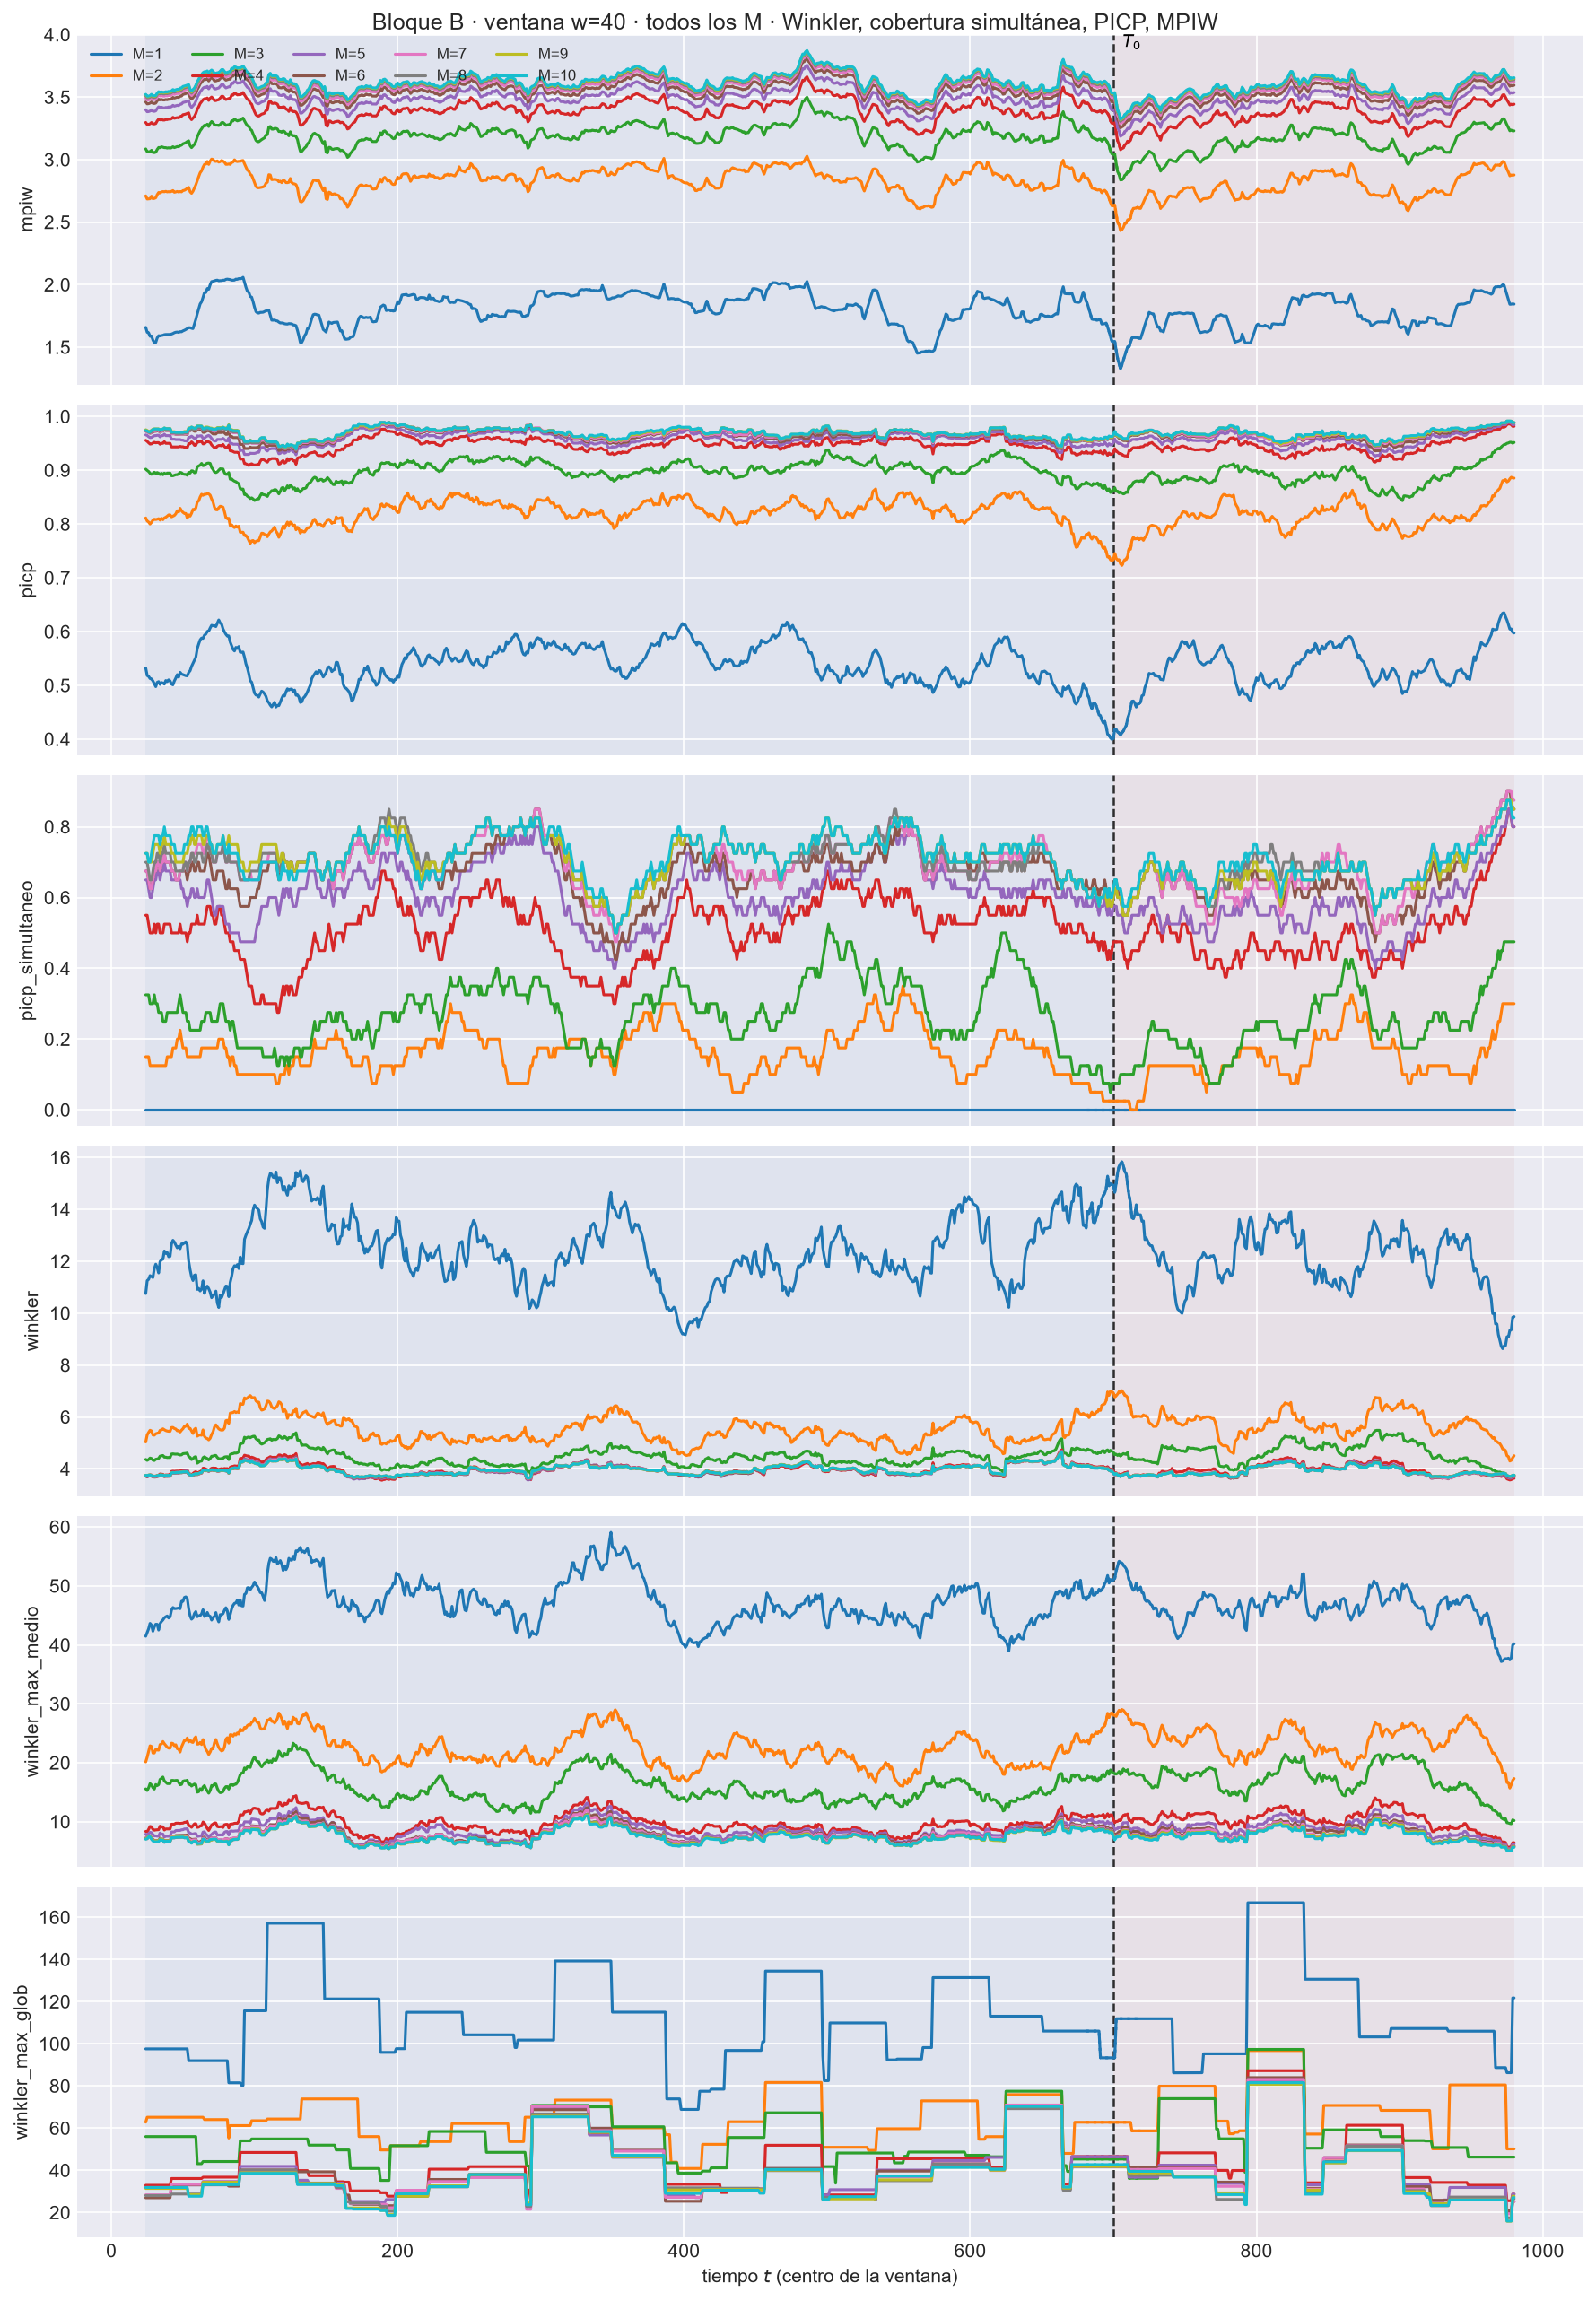
\includegraphics[width=\textwidth]{IMG/aneB_00/aneB_00_bloqueB_w40_C2.png}\end{minipage}
\caption{C-2 (TAR). Métricas de intervalo sobre la ventana móvil con $w = 20$ (izquierda) y $w = 40$ (derecha).}
\label{fig:aneB_ancho_B_C2}
\end{figure}

\begin{figure}[H]
\centering
\begin{minipage}{0.49\textwidth}\centering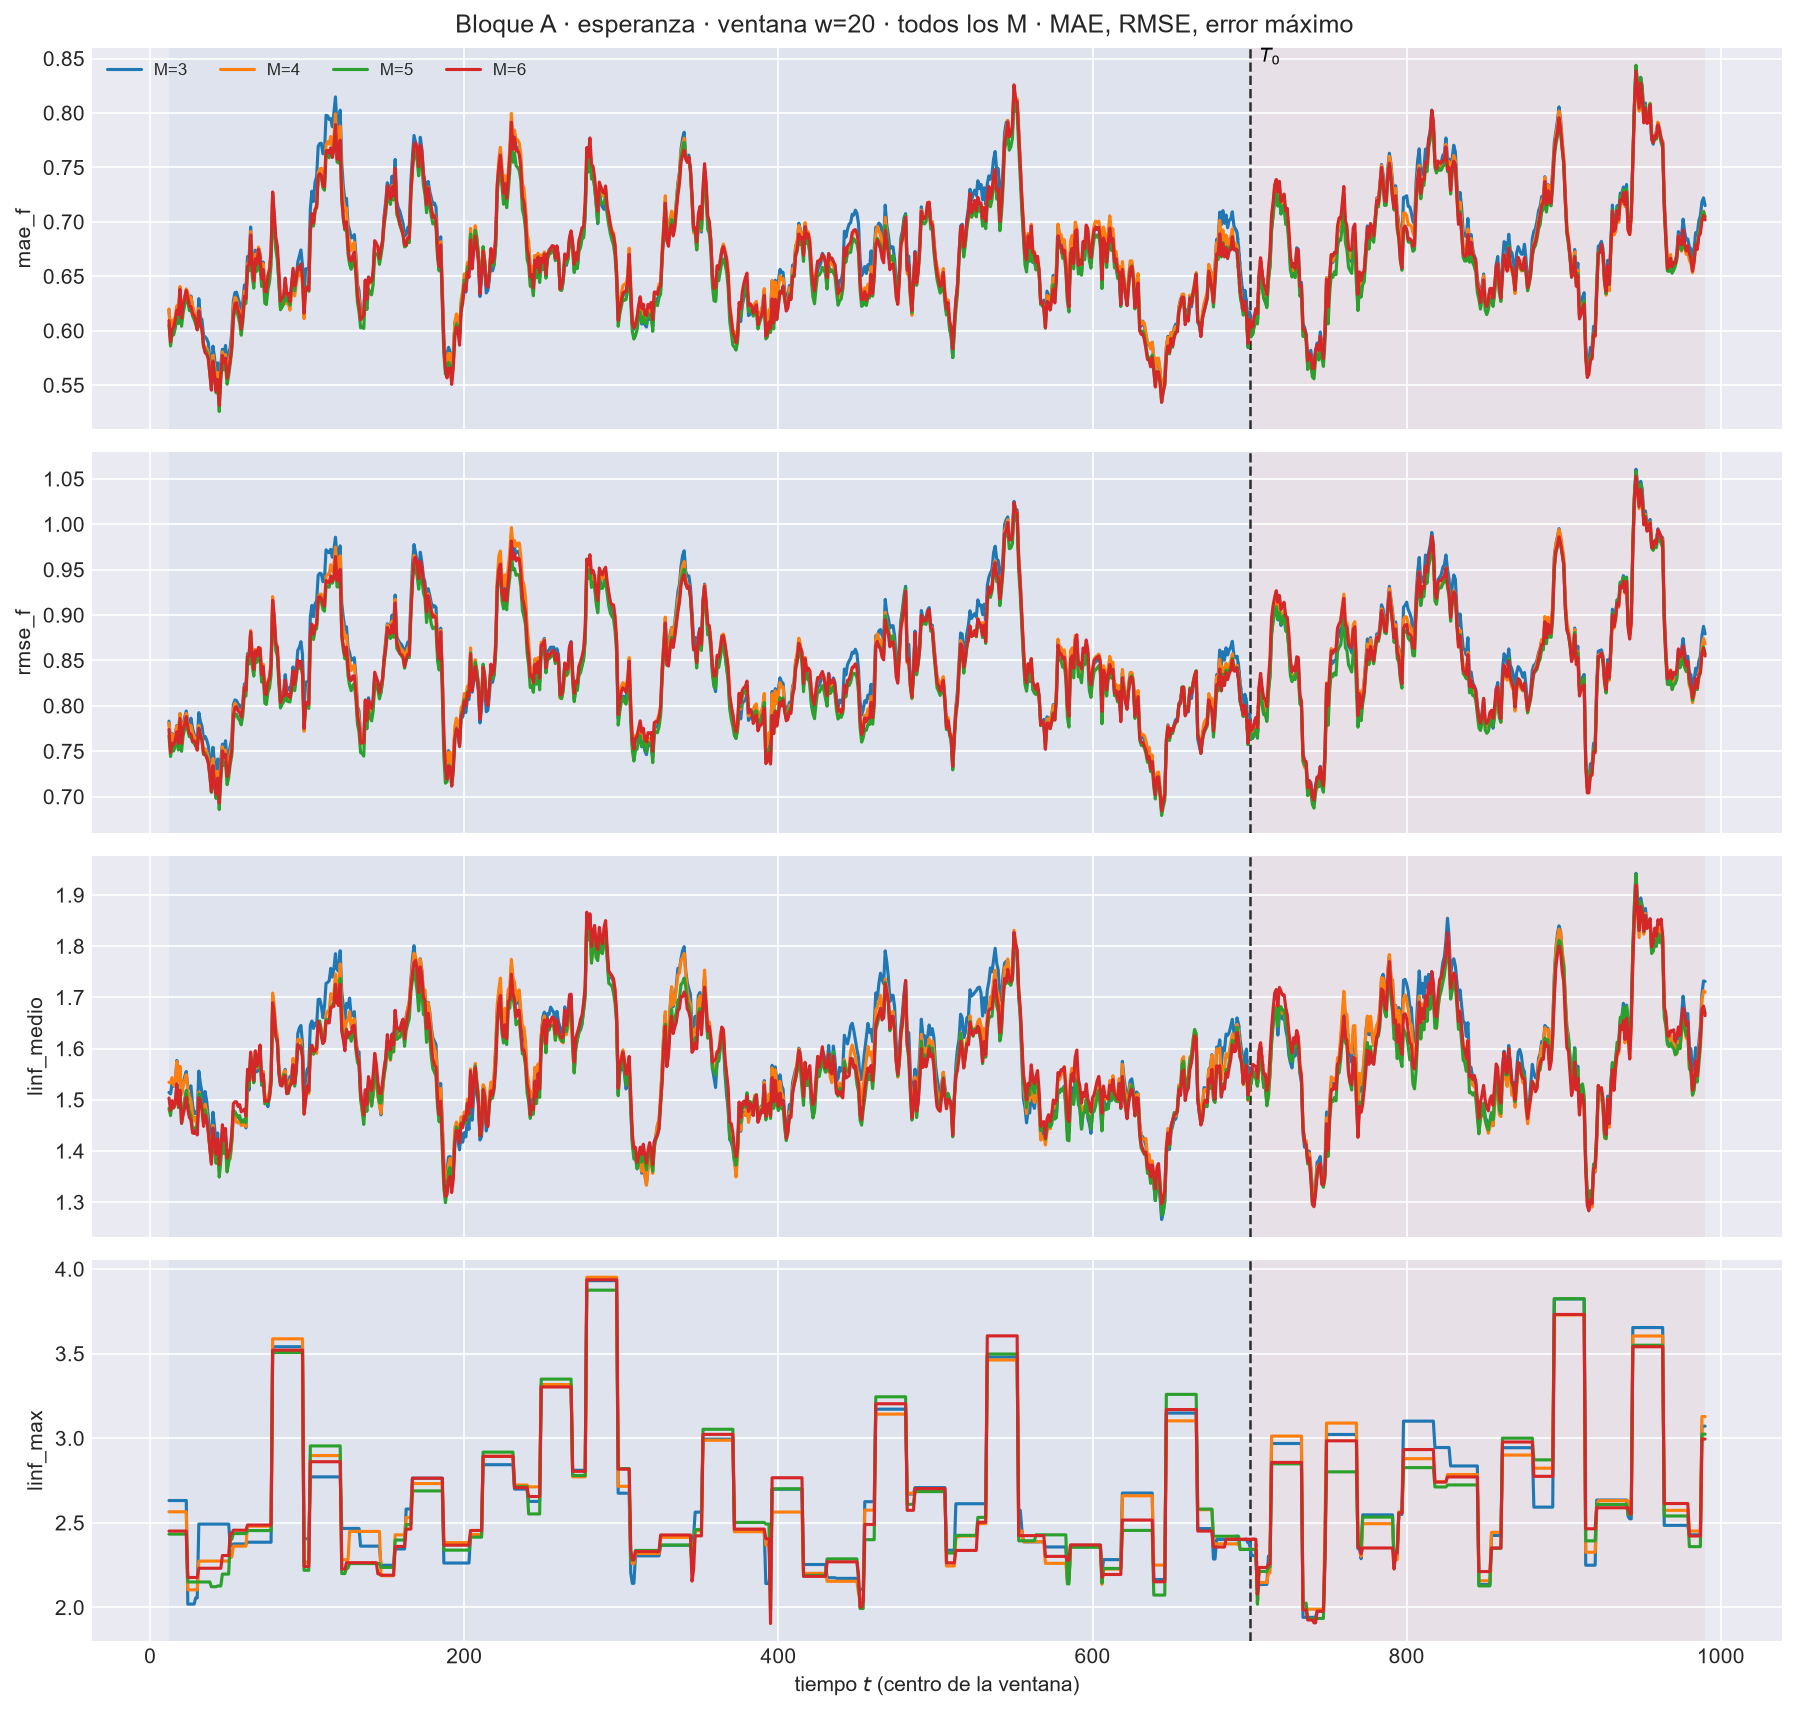
\includegraphics[width=\textwidth]{IMG/aneB_00/aneB_00_bloqueA_w20_C3.png}\end{minipage}\hfill
\begin{minipage}{0.49\textwidth}\centering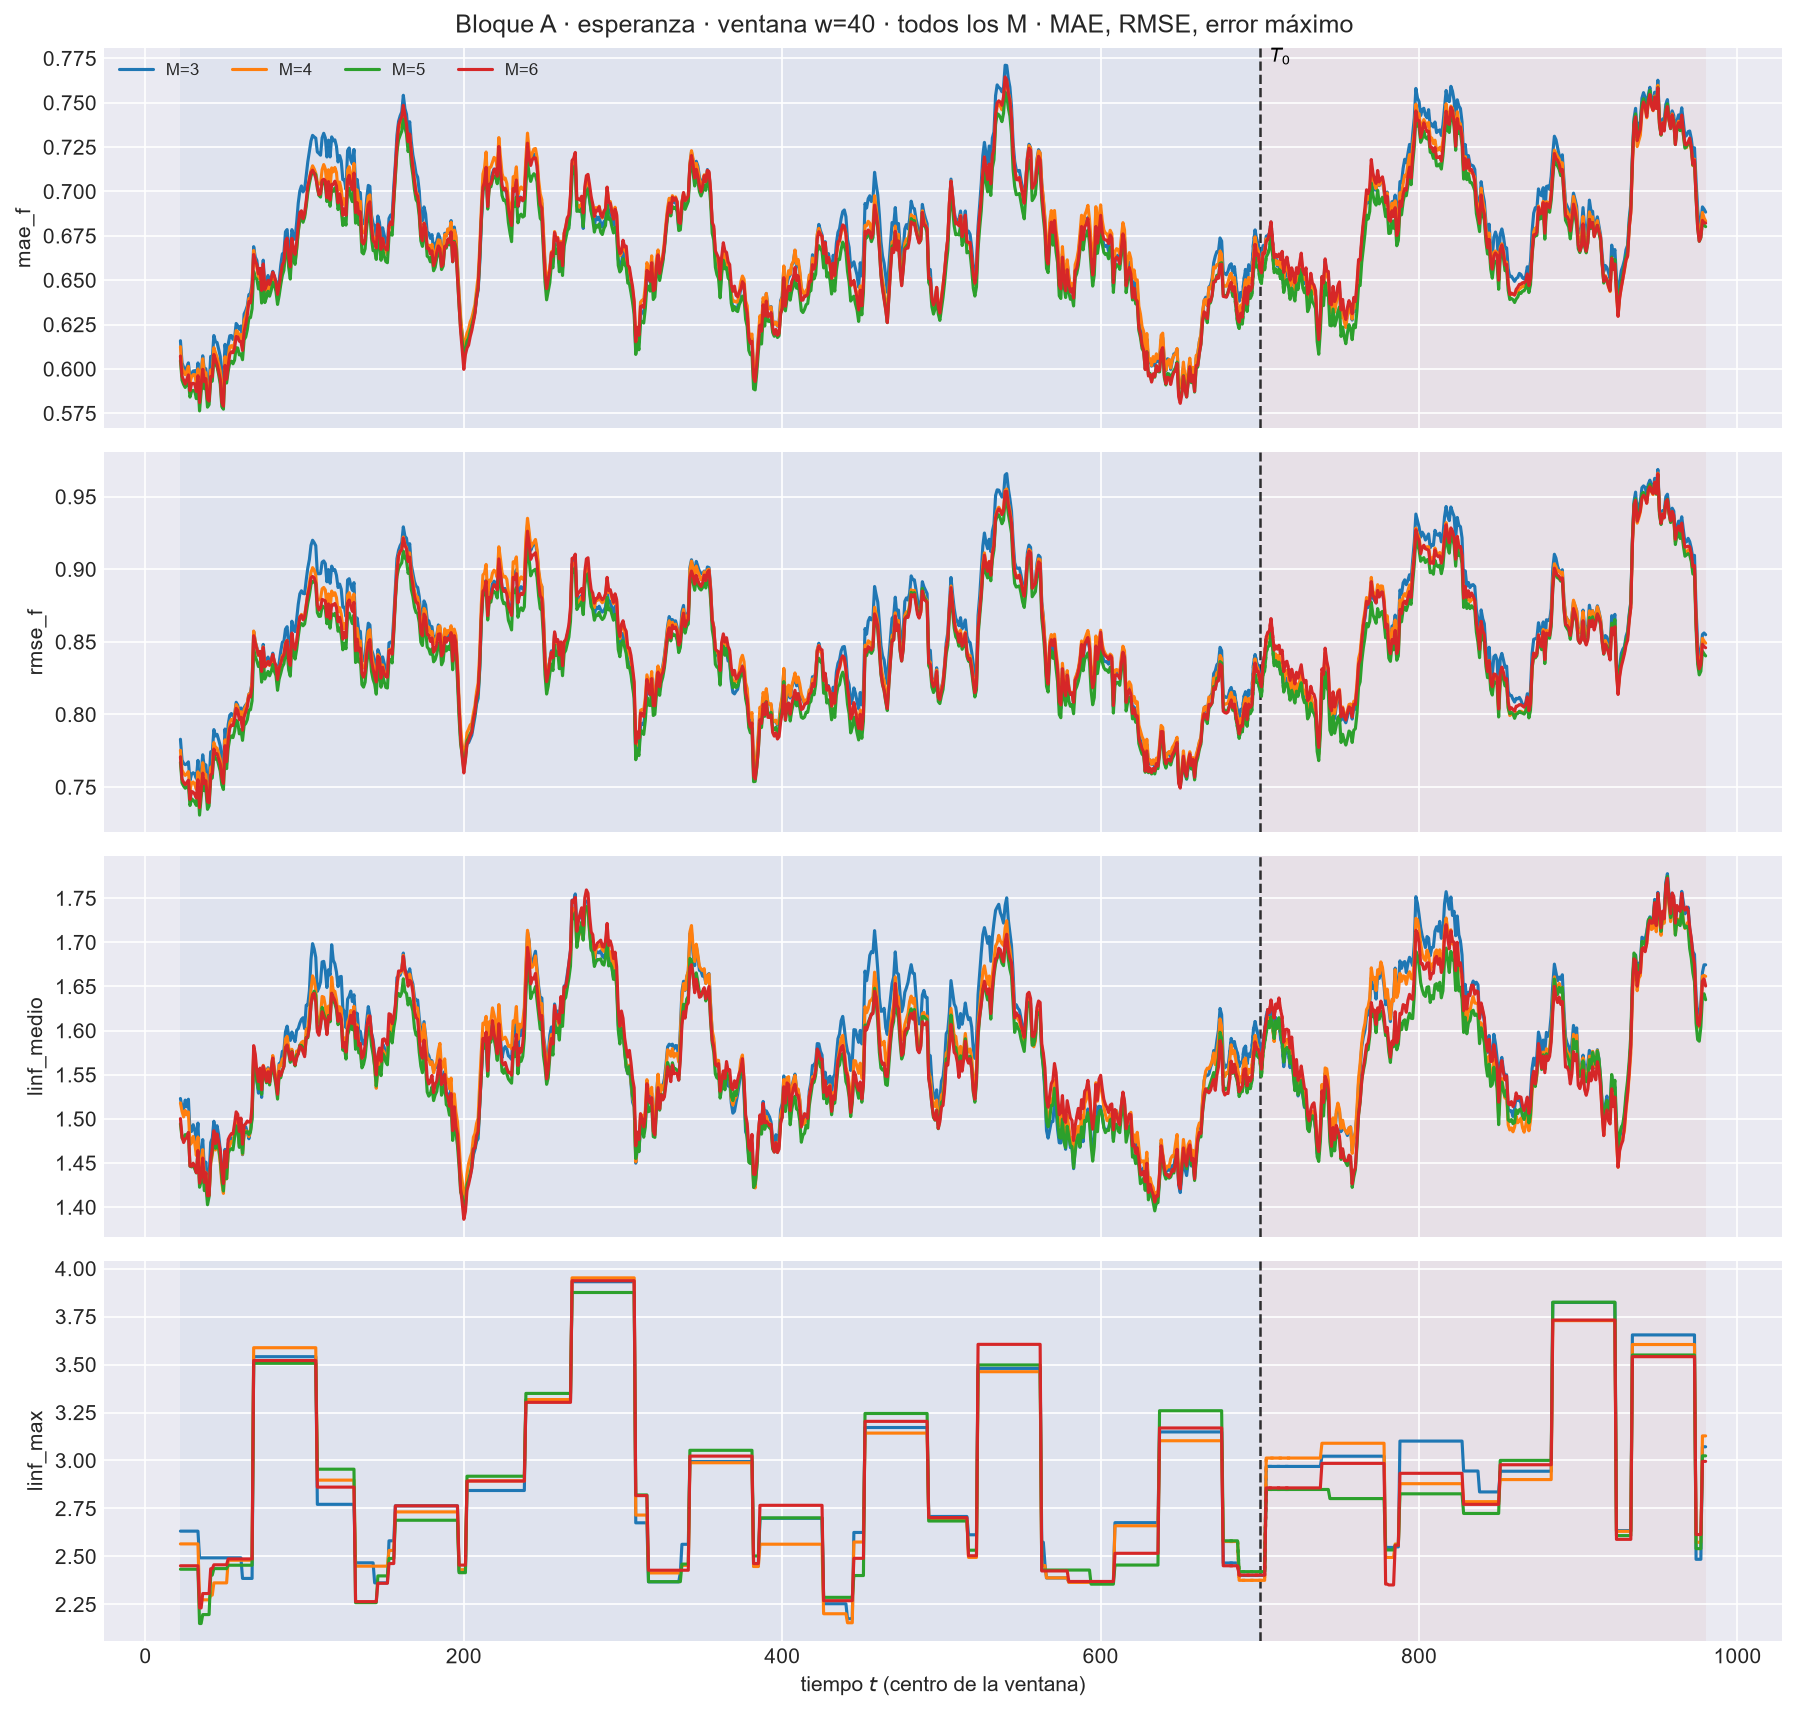
\includegraphics[width=\textwidth]{IMG/aneB_00/aneB_00_bloqueA_w40_C3.png}\end{minipage}
\caption{C-3 (multimodalidad). Métricas de error sobre la ventana móvil con $w = 20$ (izquierda) y $w = 40$ (derecha).}
\label{fig:aneB_ancho_A_C3}
\end{figure}

\begin{figure}[H]
\centering
\begin{minipage}{0.49\textwidth}\centering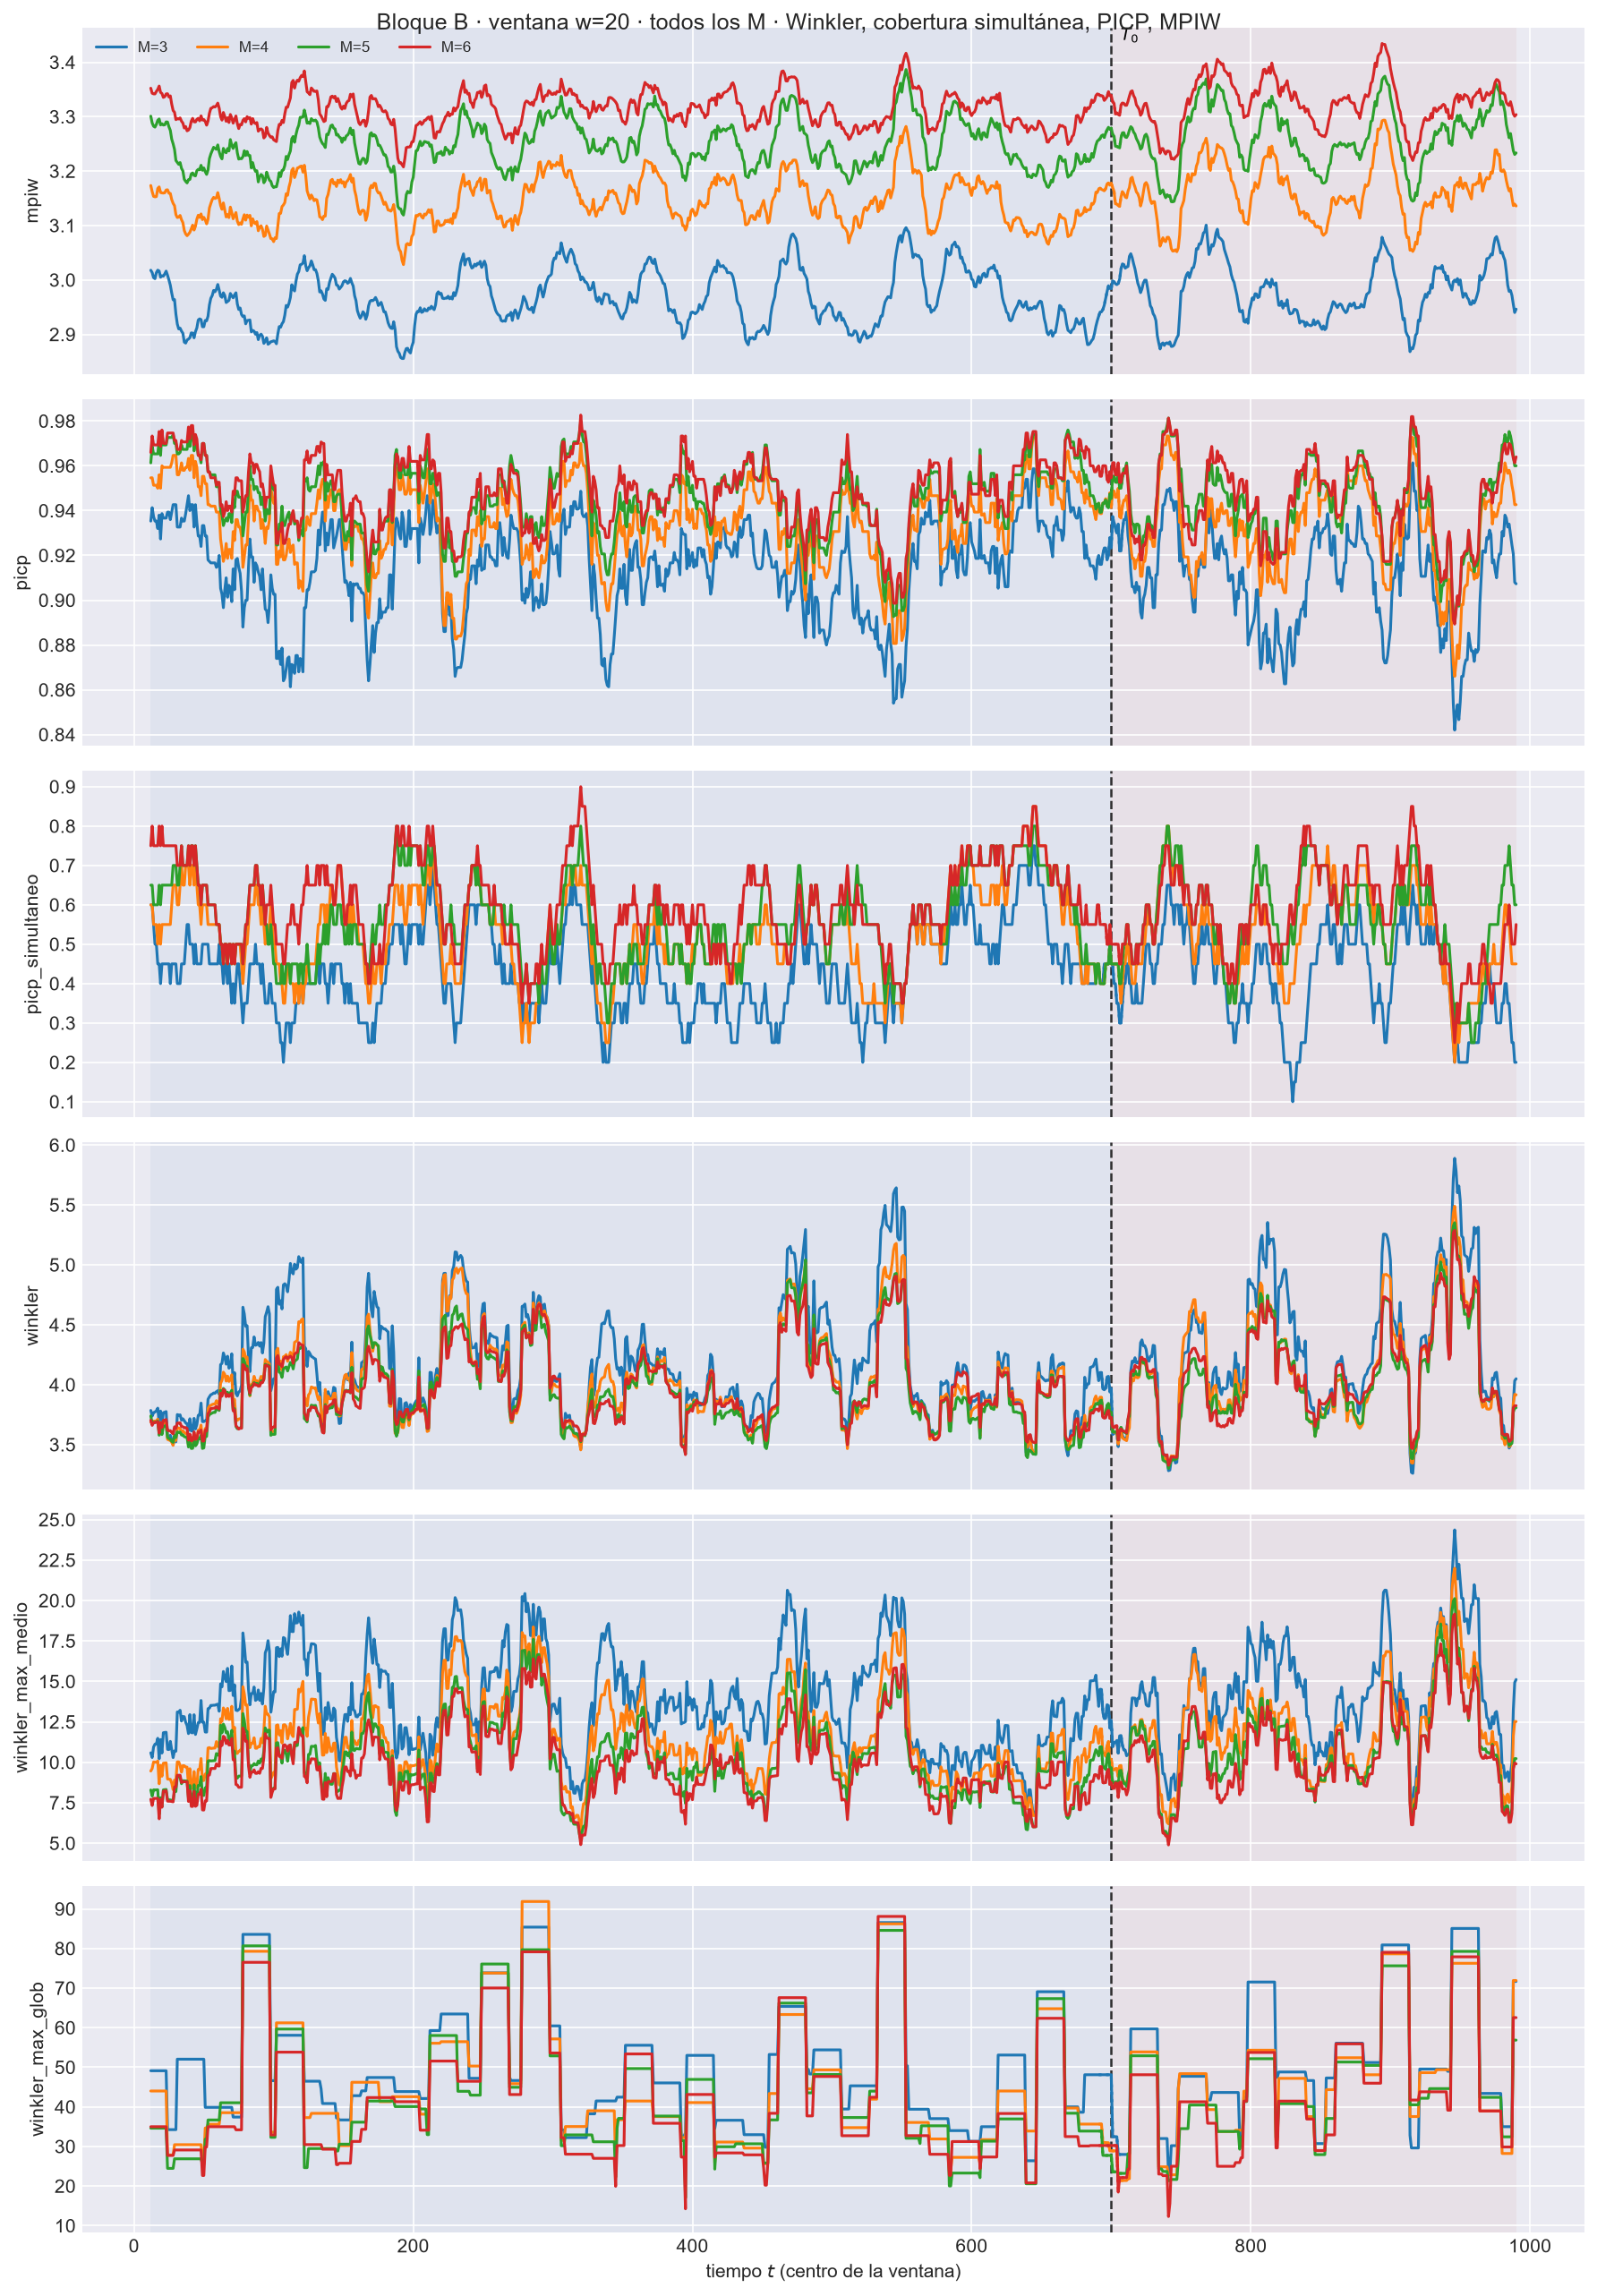
\includegraphics[width=\textwidth]{IMG/aneB_00/aneB_00_bloqueB_w20_C3.png}\end{minipage}\hfill
\begin{minipage}{0.49\textwidth}\centering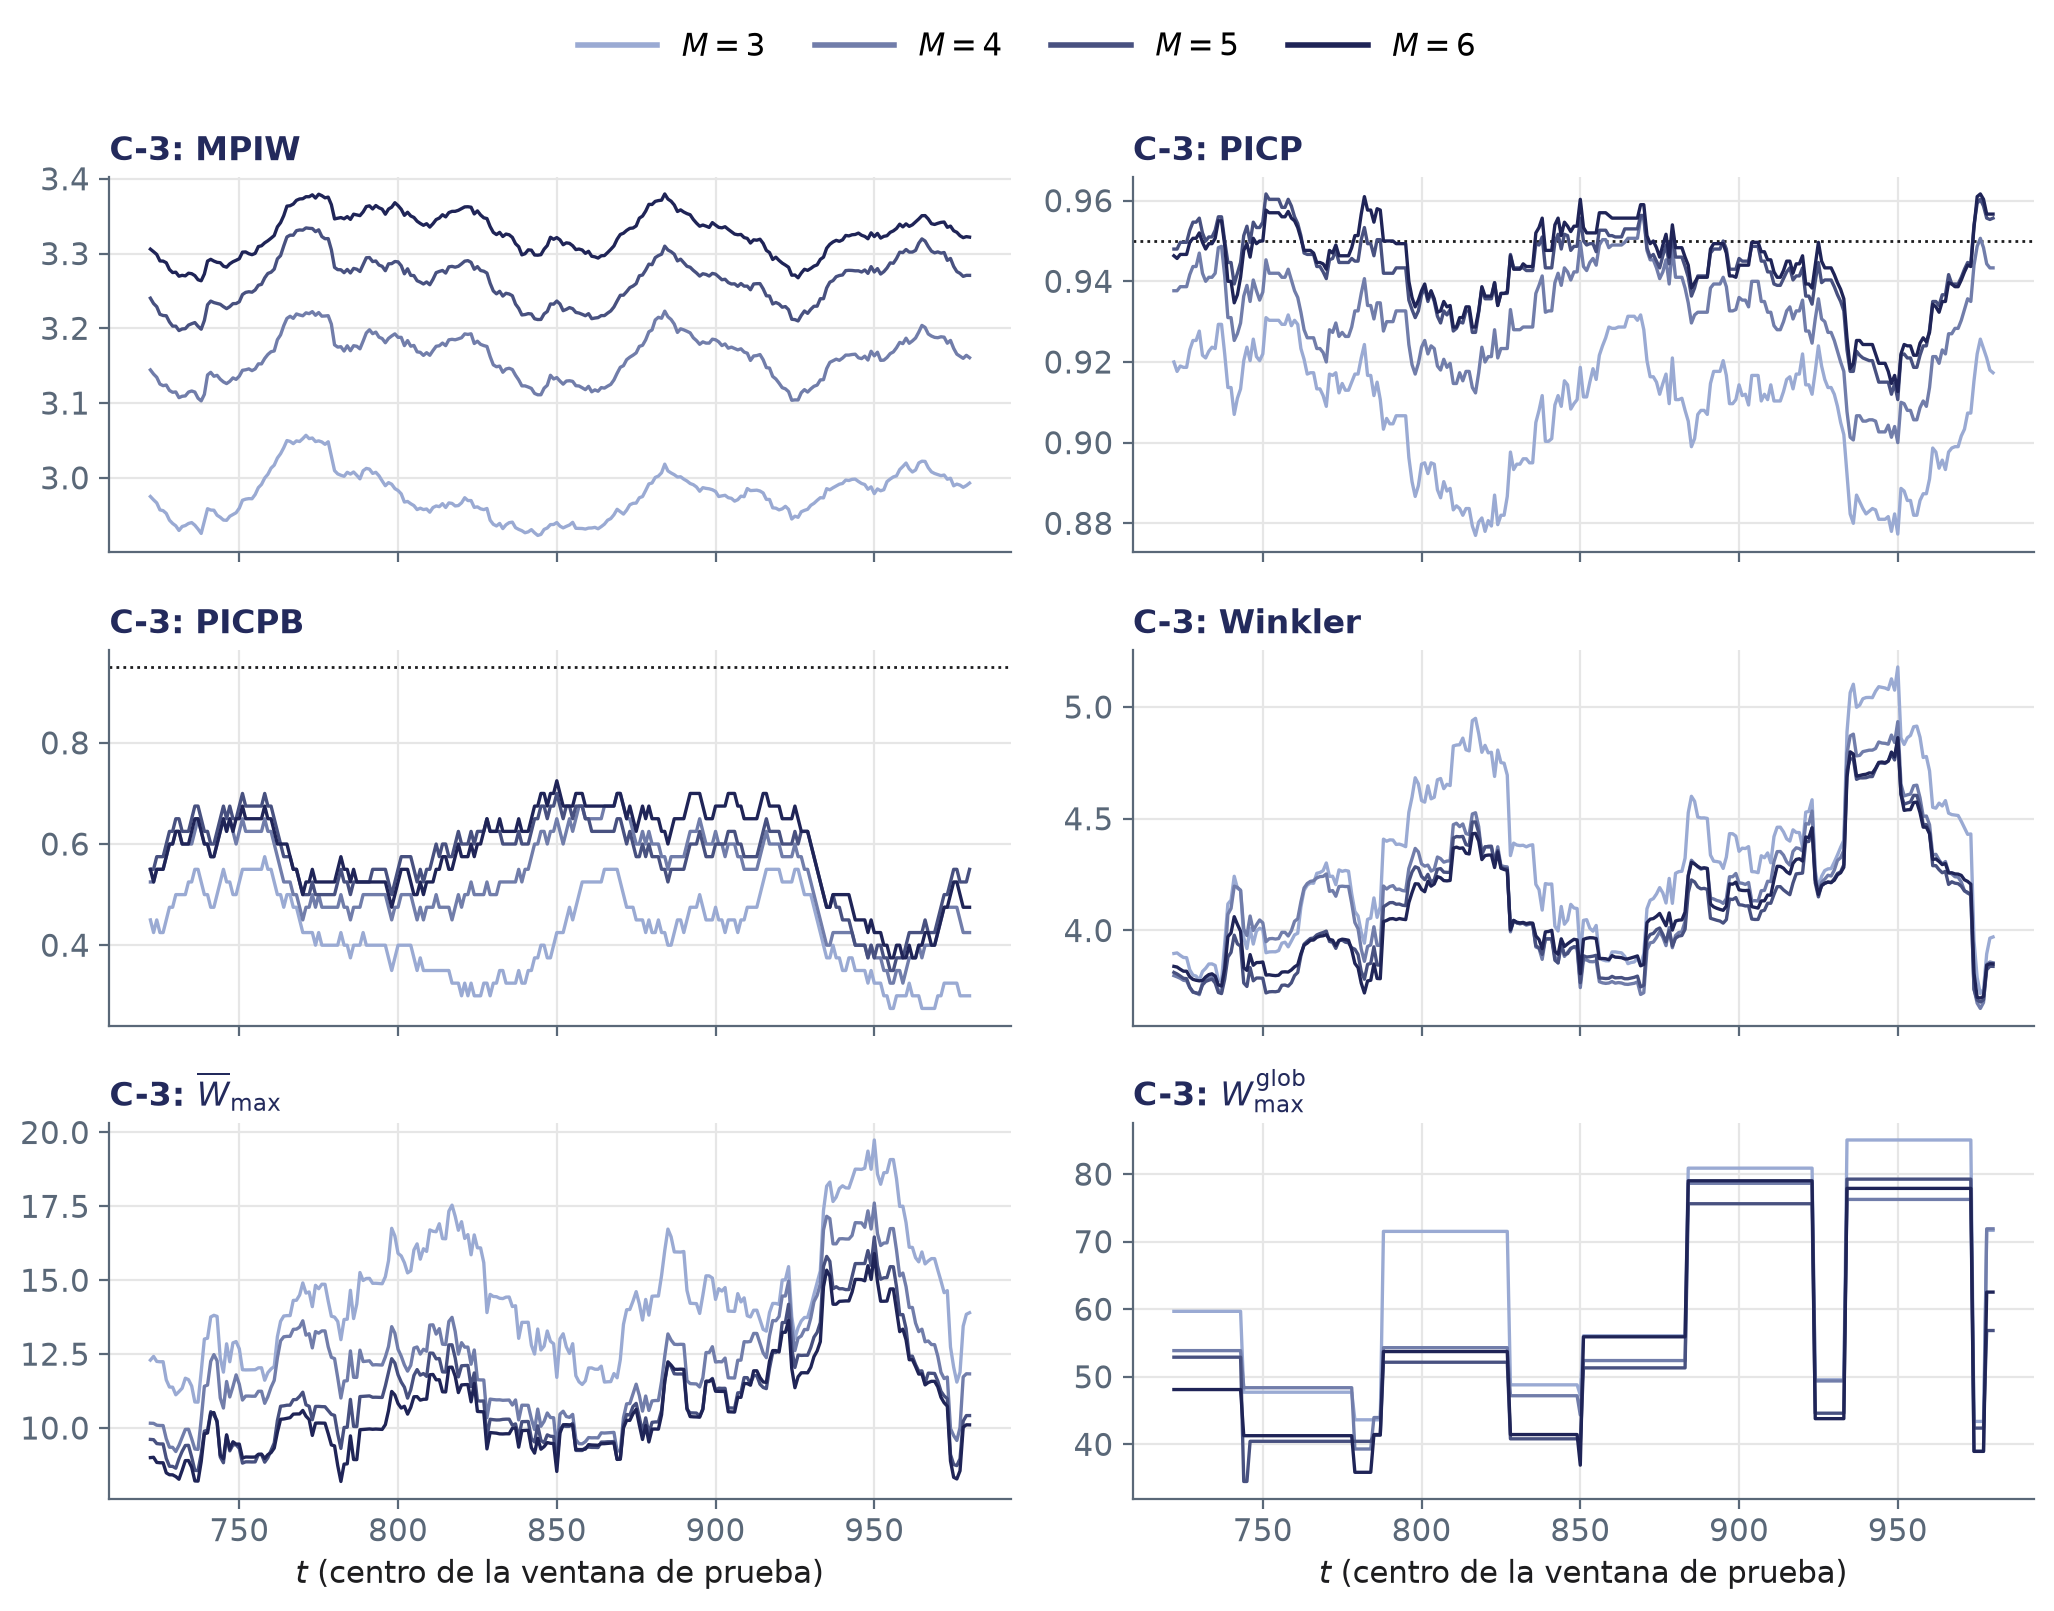
\includegraphics[width=\textwidth]{IMG/aneB_00/aneB_00_bloqueB_w40_C3.png}\end{minipage}
\caption{C-3 (multimodalidad). Métricas de intervalo sobre la ventana móvil con $w = 20$ (izquierda) y $w = 40$ (derecha).}
\label{fig:aneB_ancho_B_C3}
\end{figure}

\section{Desempeño a lo largo del período de prueba}
\label{aneB_00_03_desempeno_por_ventana}

\subsection{Error de predicción}
\label{aneB_00_03_01_ventana_error}

Error de la ventana móvil ($w = 30$) de los predictores puntuales del PSBPM-FD y de las referencias.

\begin{figure}[H]
\centering
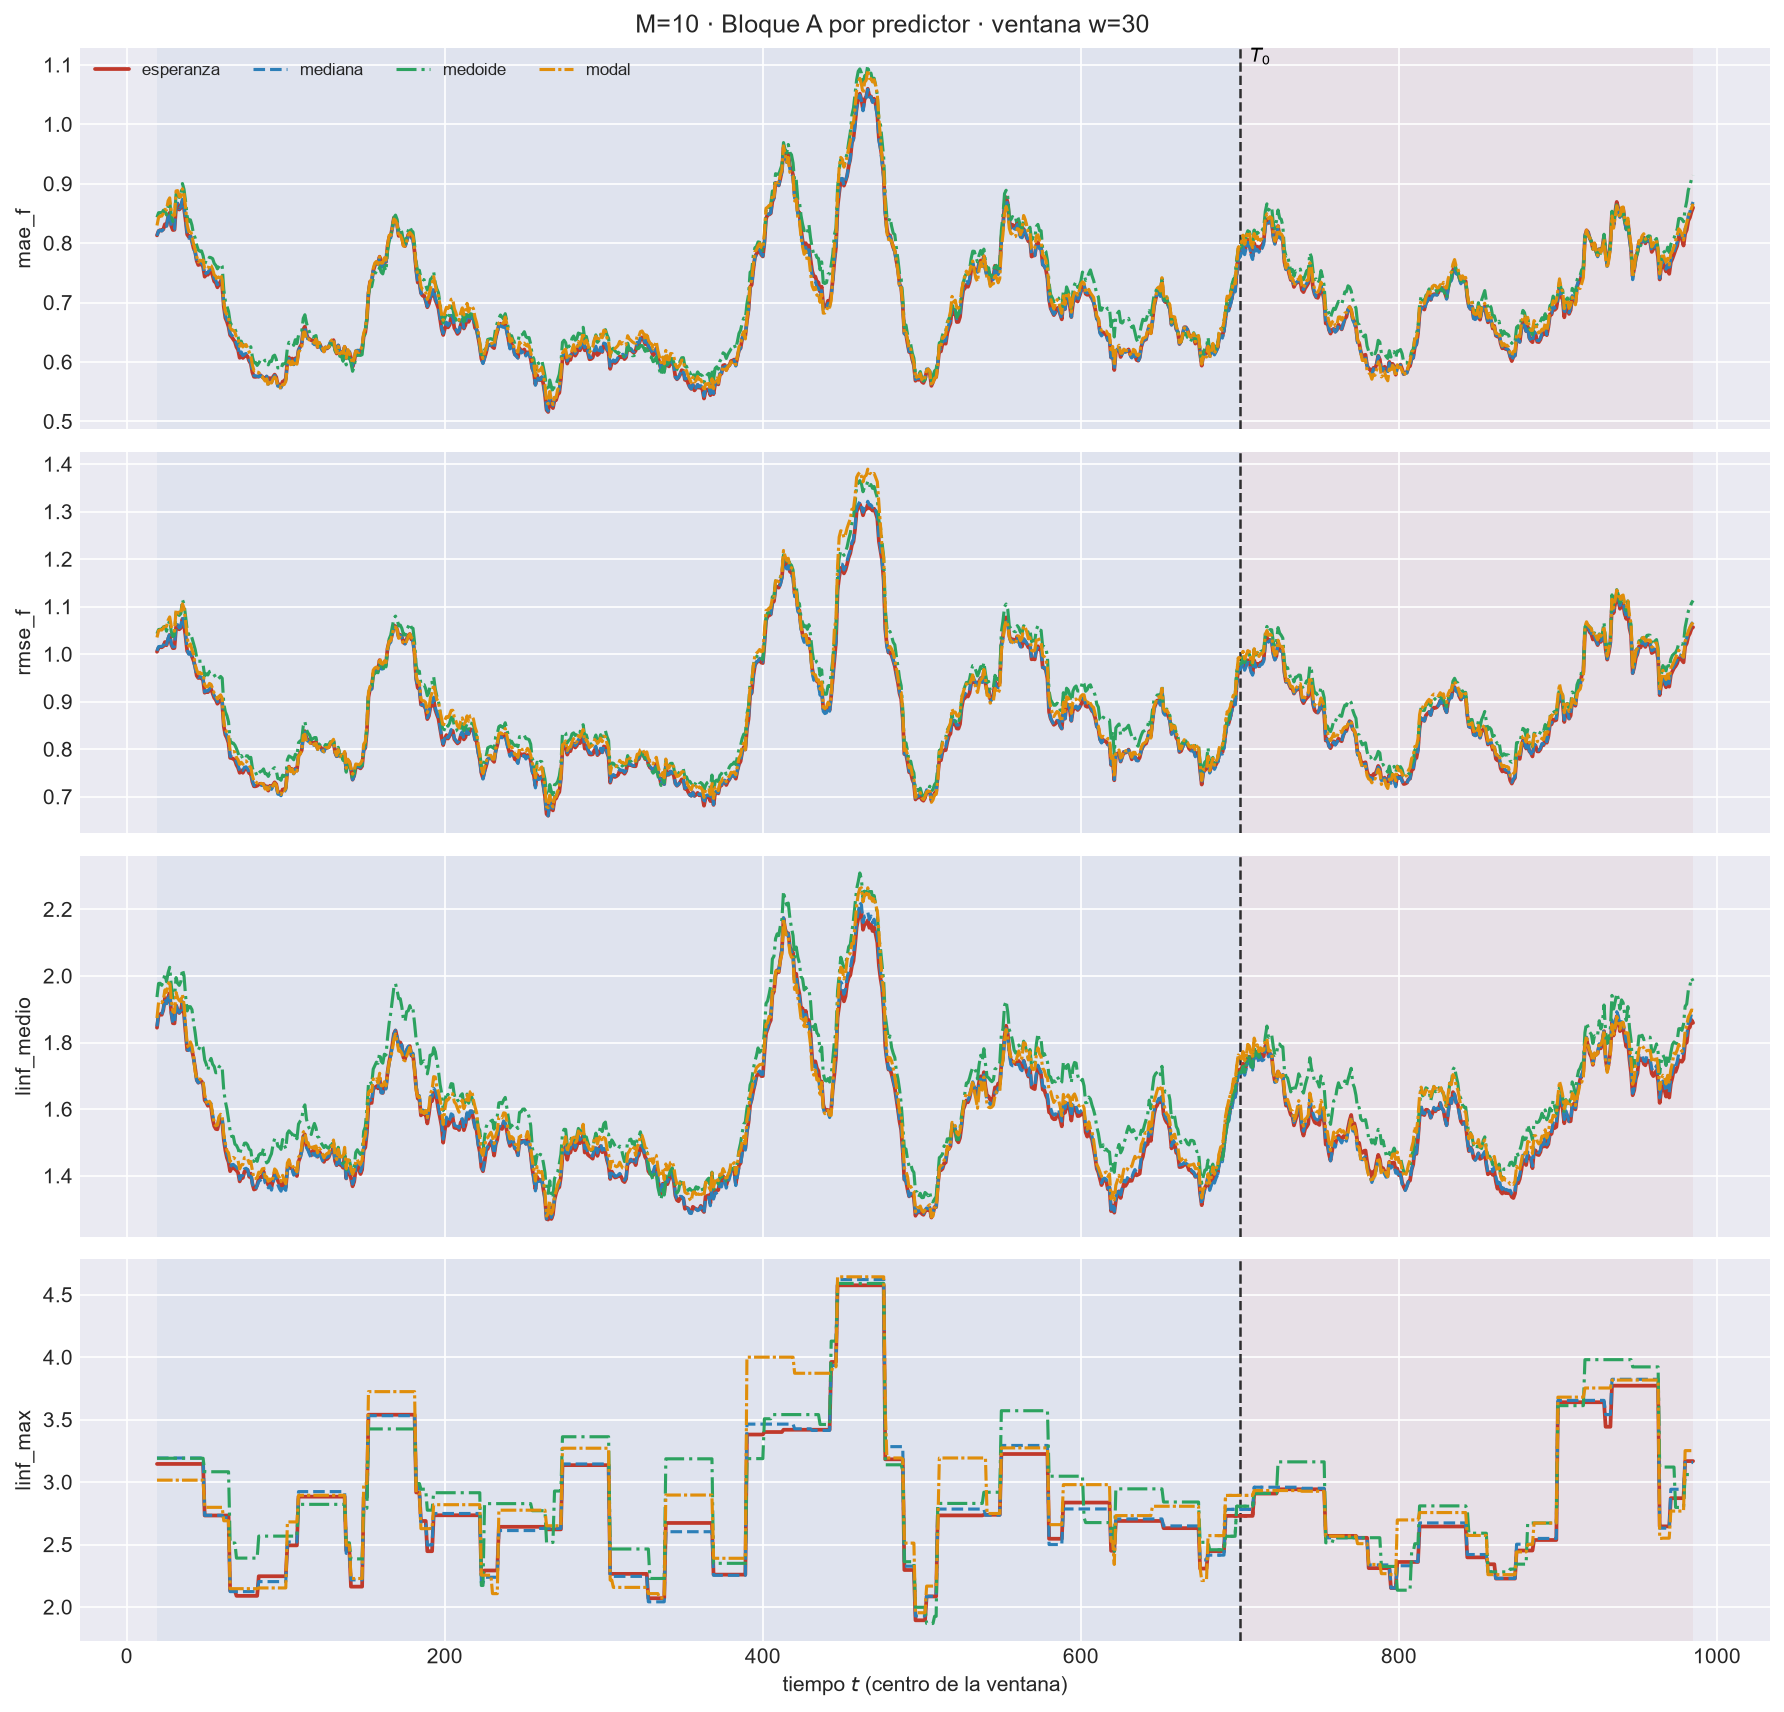
\includegraphics[width=\textwidth,height=0.8\textheight,keepaspectratio]{IMG/aneB_00/aneB_00_ventana_predictores_w30_C1.png}
\caption{C-1 (GARCH). Error de los predictores puntuales sobre la ventana móvil ($M_{\mathrm{ref}}$).}
\label{fig:aneB_pred_C1}
\end{figure}

\begin{figure}[H]
\centering
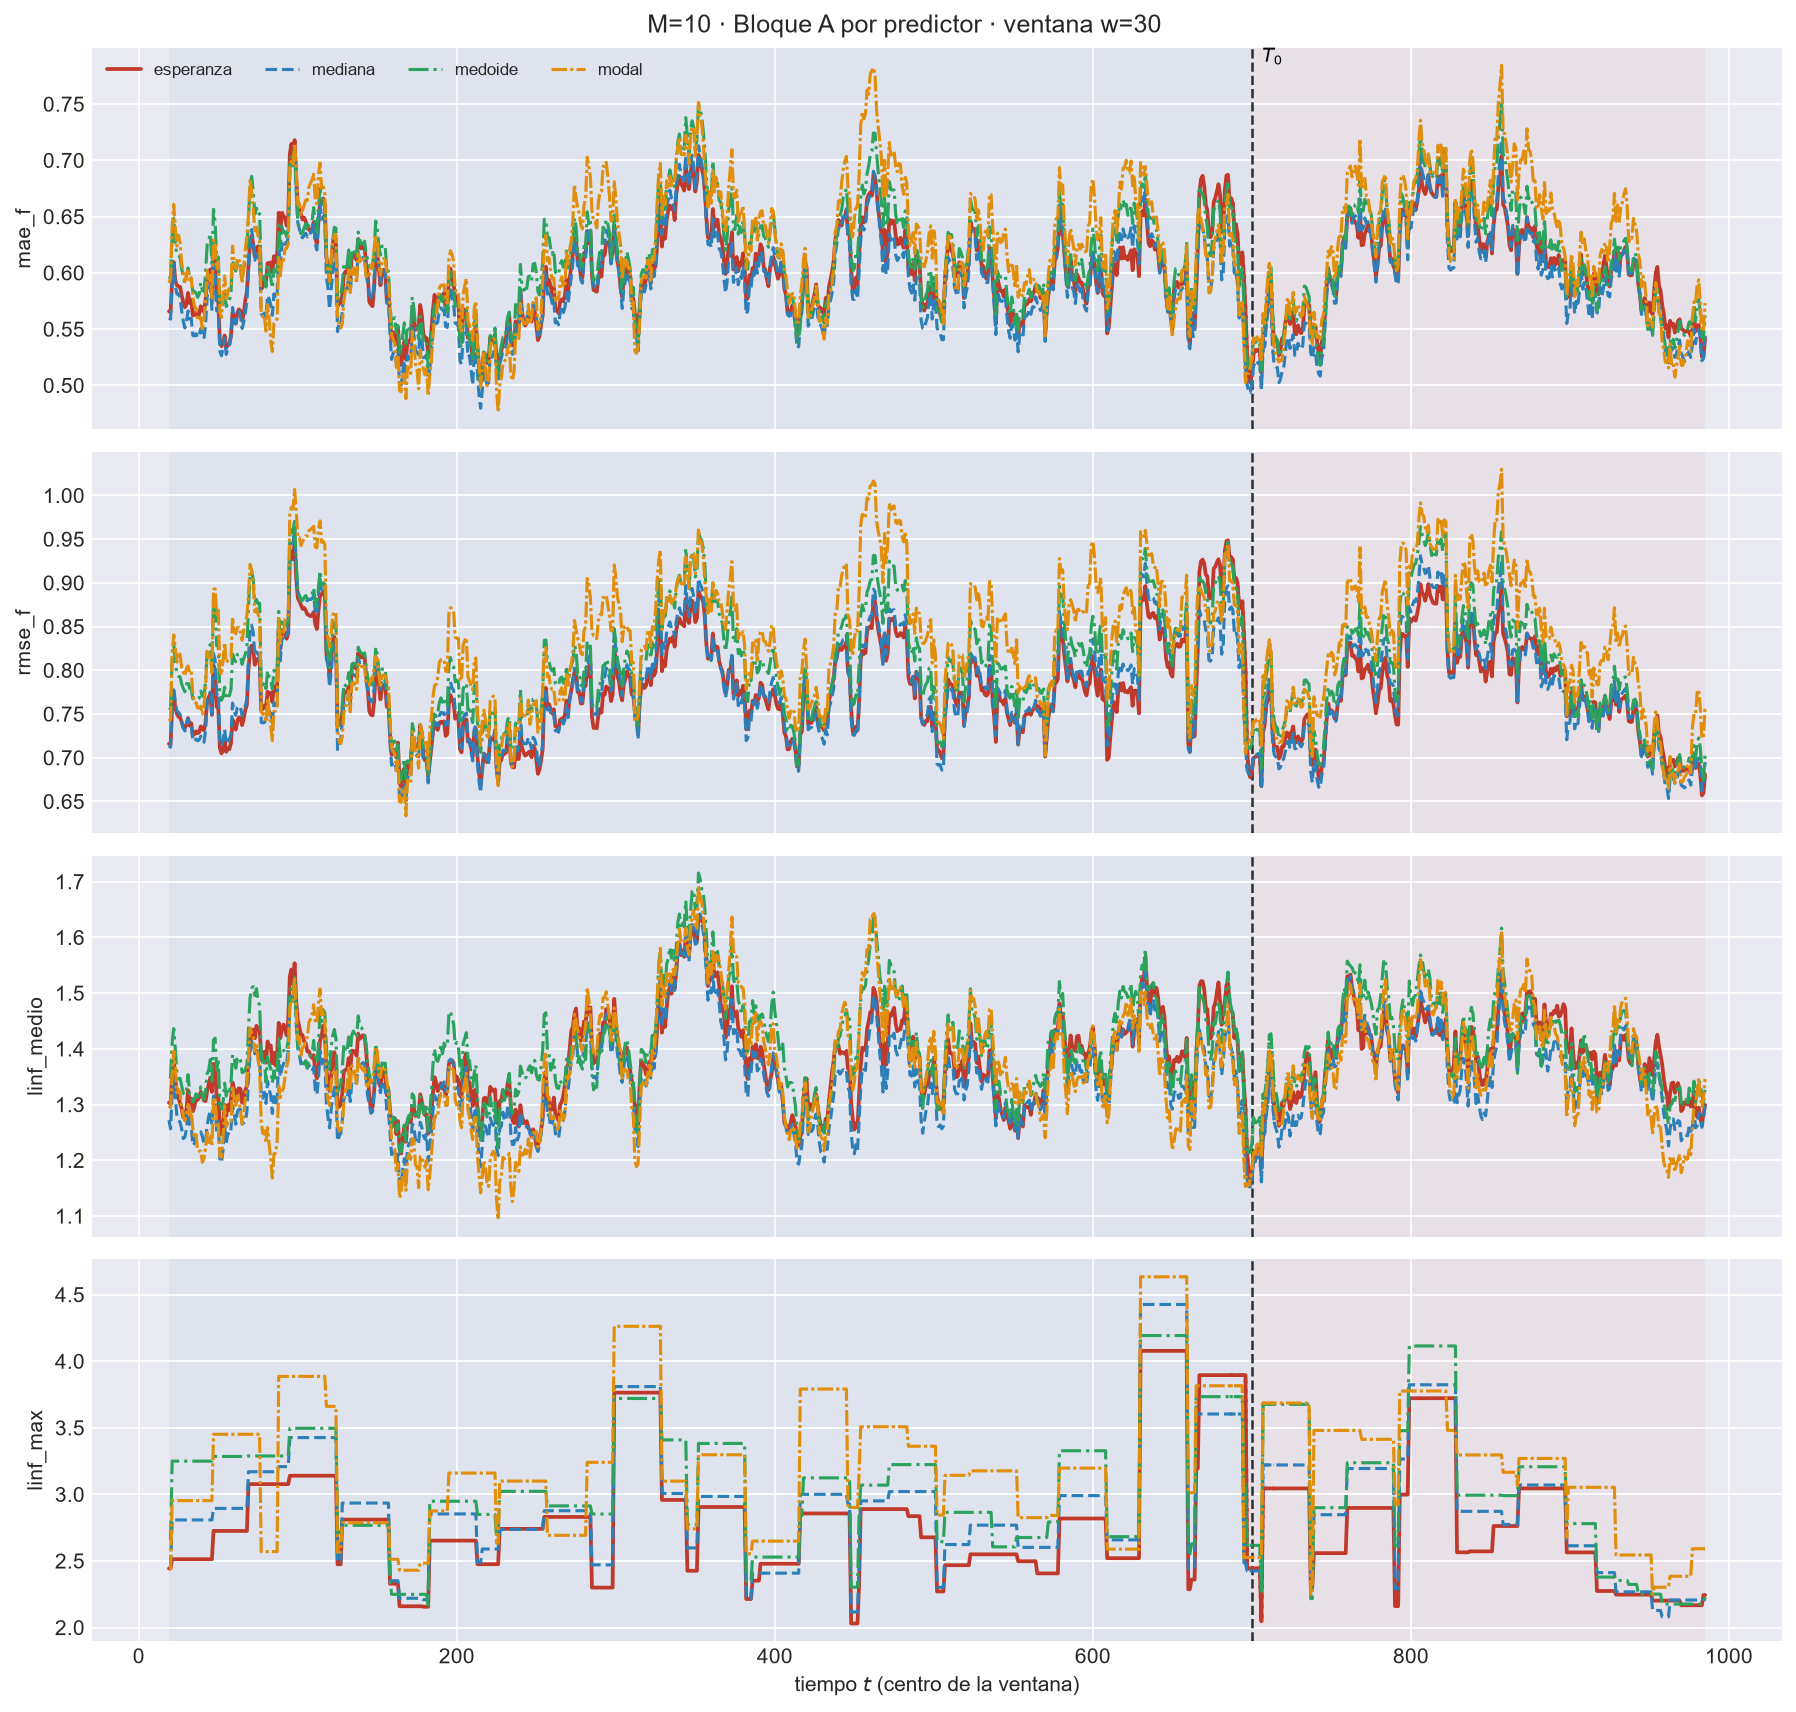
\includegraphics[width=\textwidth,height=0.8\textheight,keepaspectratio]{IMG/aneB_00/aneB_00_ventana_predictores_w30_C2.png}
\caption{C-2 (TAR). Error de los predictores puntuales sobre la ventana móvil ($M_{\mathrm{ref}}$).}
\label{fig:aneB_pred_C2}
\end{figure}

\begin{figure}[H]
\centering
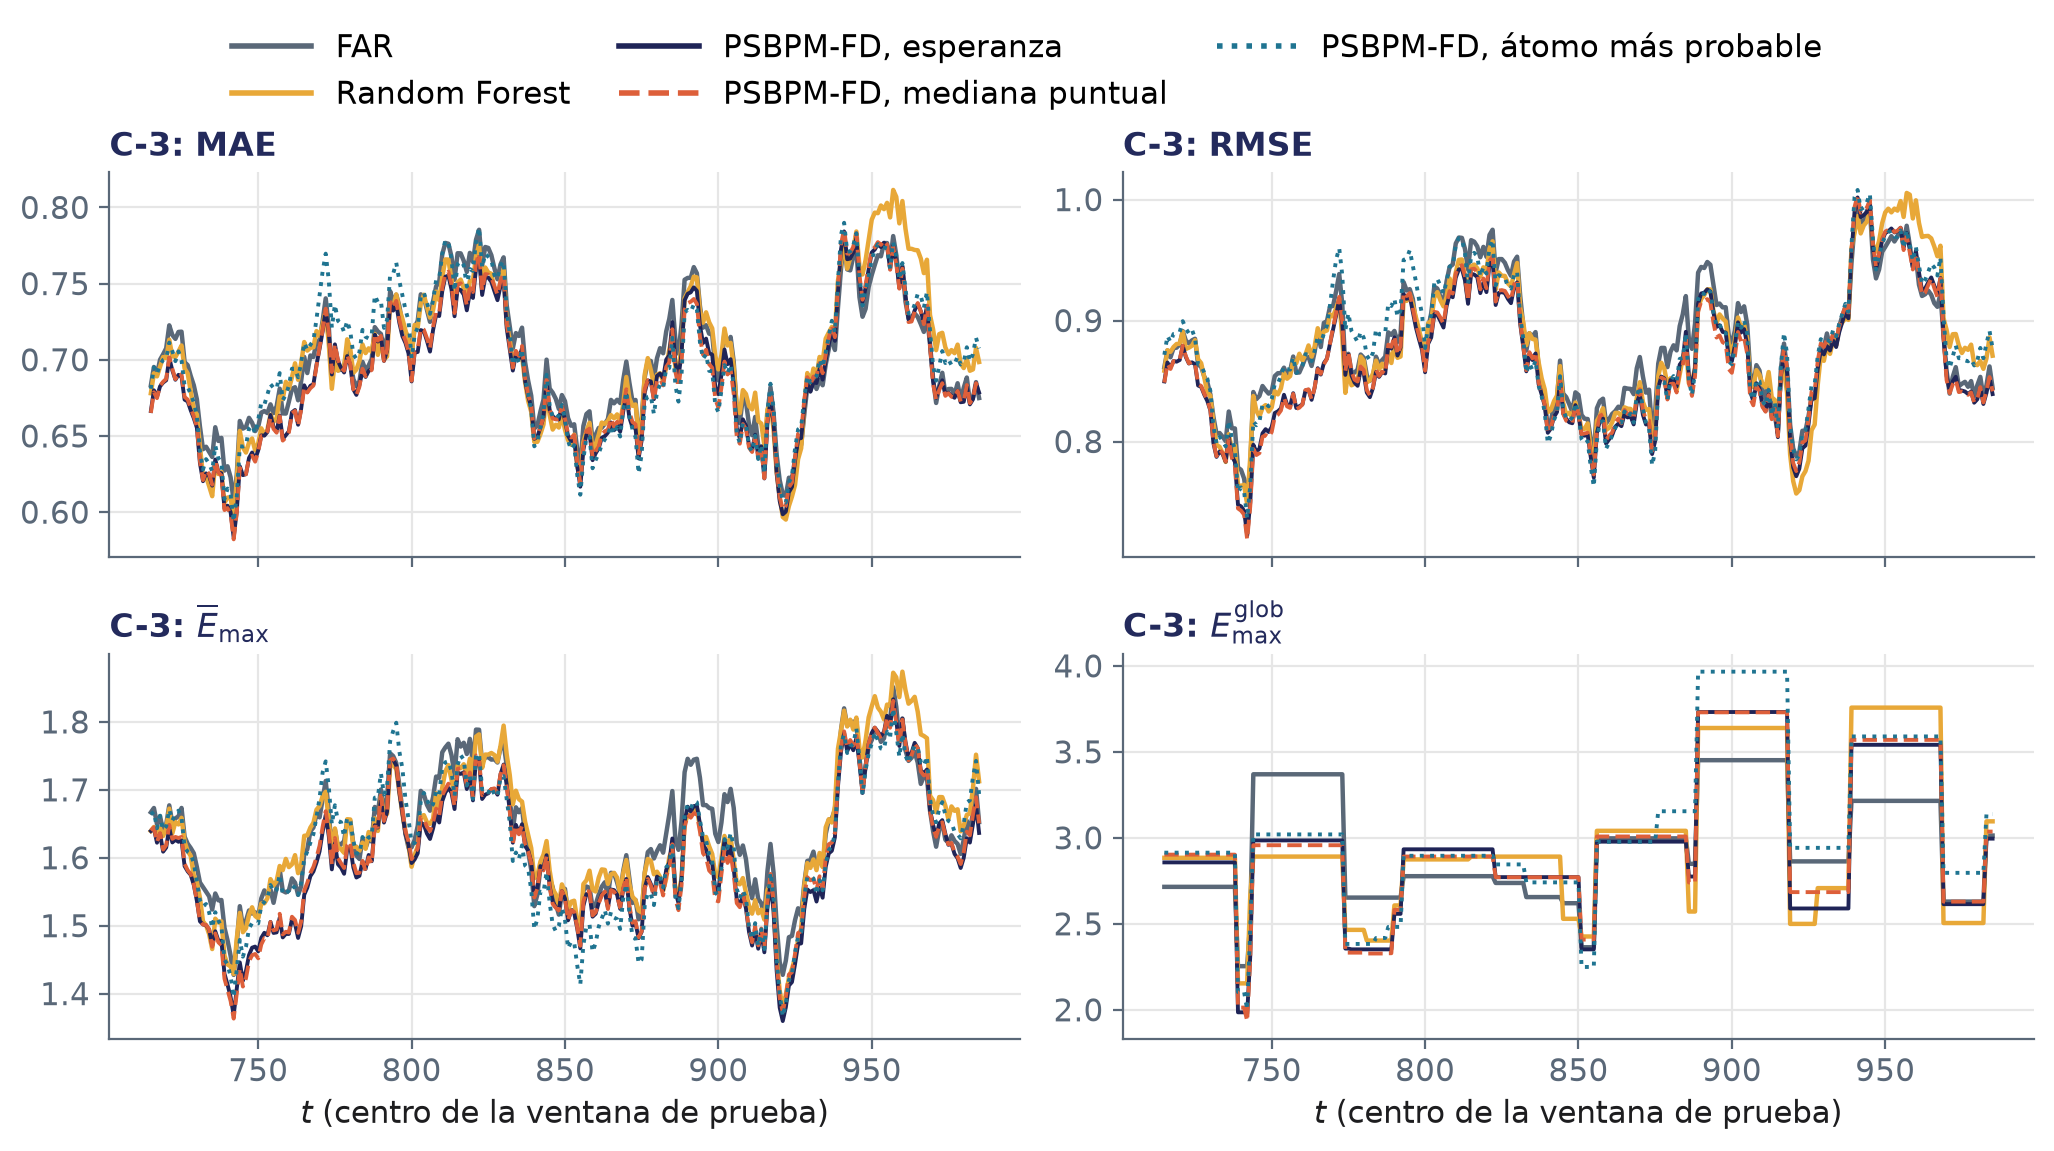
\includegraphics[width=\textwidth,height=0.8\textheight,keepaspectratio]{IMG/aneB_00/aneB_00_ventana_predictores_w30_C3.png}
\caption{C-3 (multimodalidad). Error de los predictores puntuales sobre la ventana móvil ($M_{\mathrm{ref}}$).}
\label{fig:aneB_pred_C3}
\end{figure}

\subsection{Intervalos de predicción}
\label{aneB_00_03_02_ventana_intervalos}

Métricas de intervalo de la ventana móvil ($w = 30$) de las tres construcciones del PSBPM-FD y del FAR.

\begin{figure}[H]
\centering
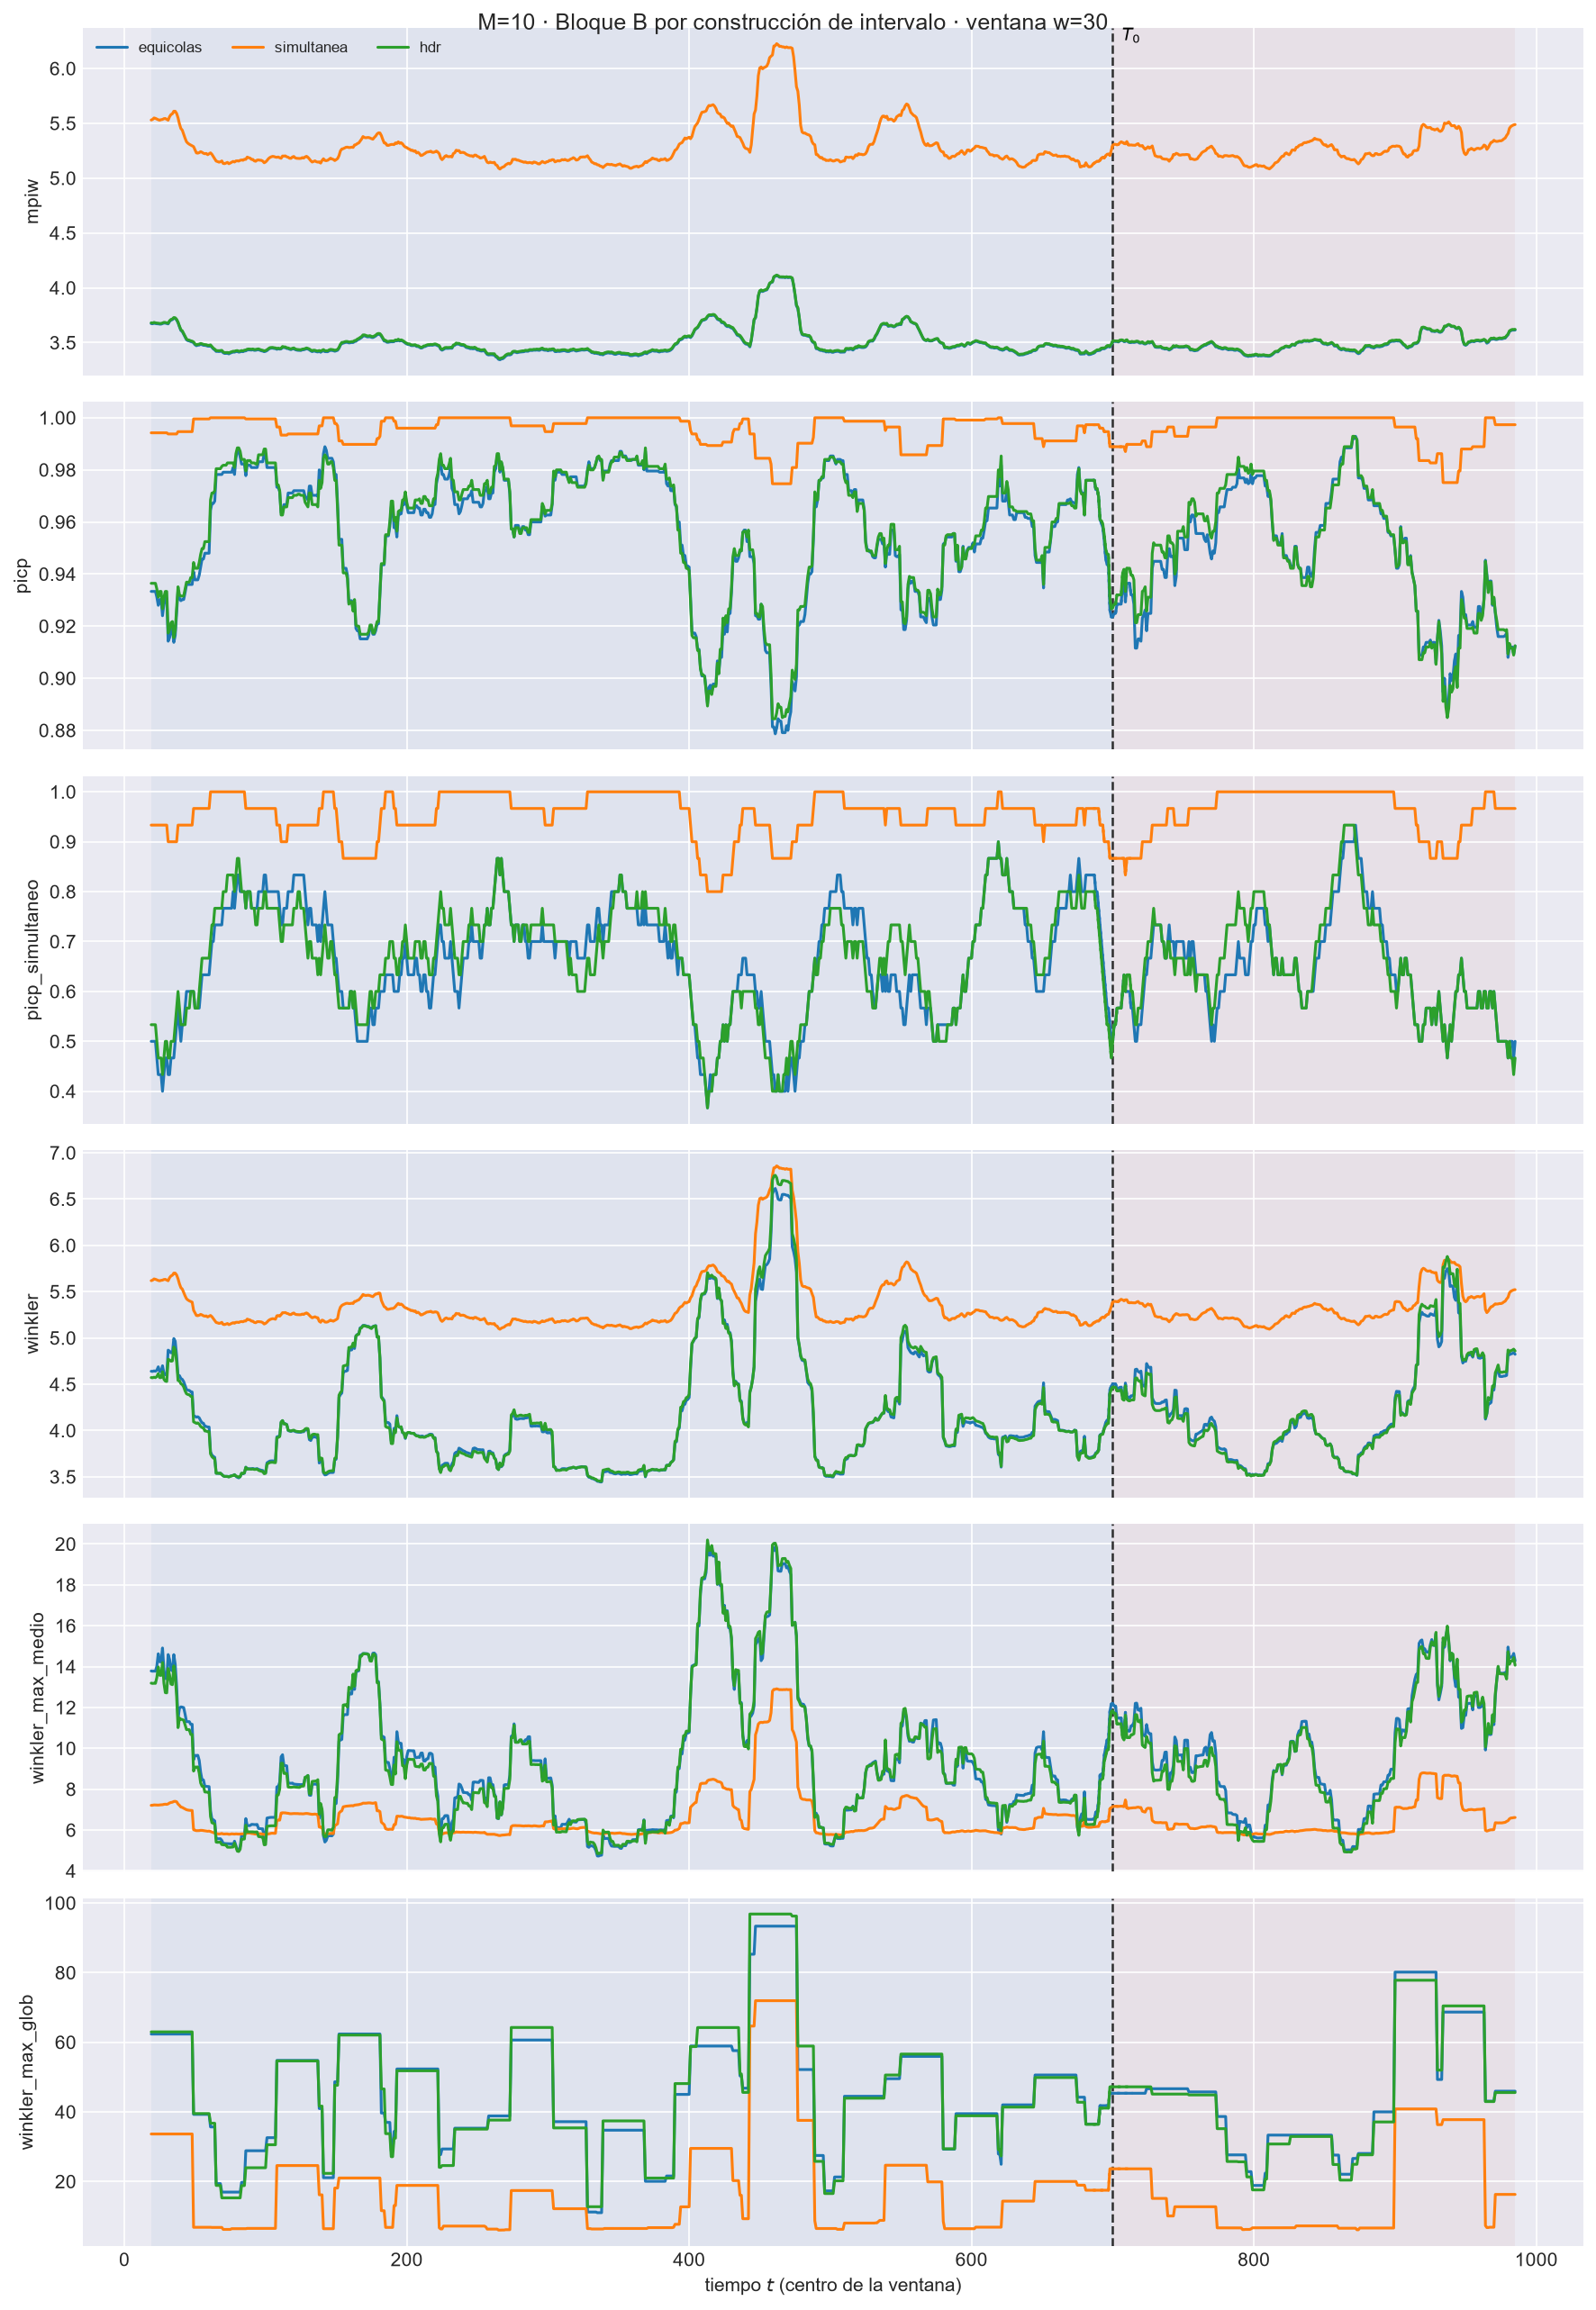
\includegraphics[width=\textwidth,height=0.75\textheight,keepaspectratio]{IMG/aneB_00/aneB_00_ventana_intervalos_w30_C1.png}
\caption{C-1 (GARCH). Métricas de intervalo sobre la ventana móvil ($M_{\mathrm{ref}}$).}
\label{fig:aneB_int_C1}
\end{figure}

\begin{figure}[H]
\centering
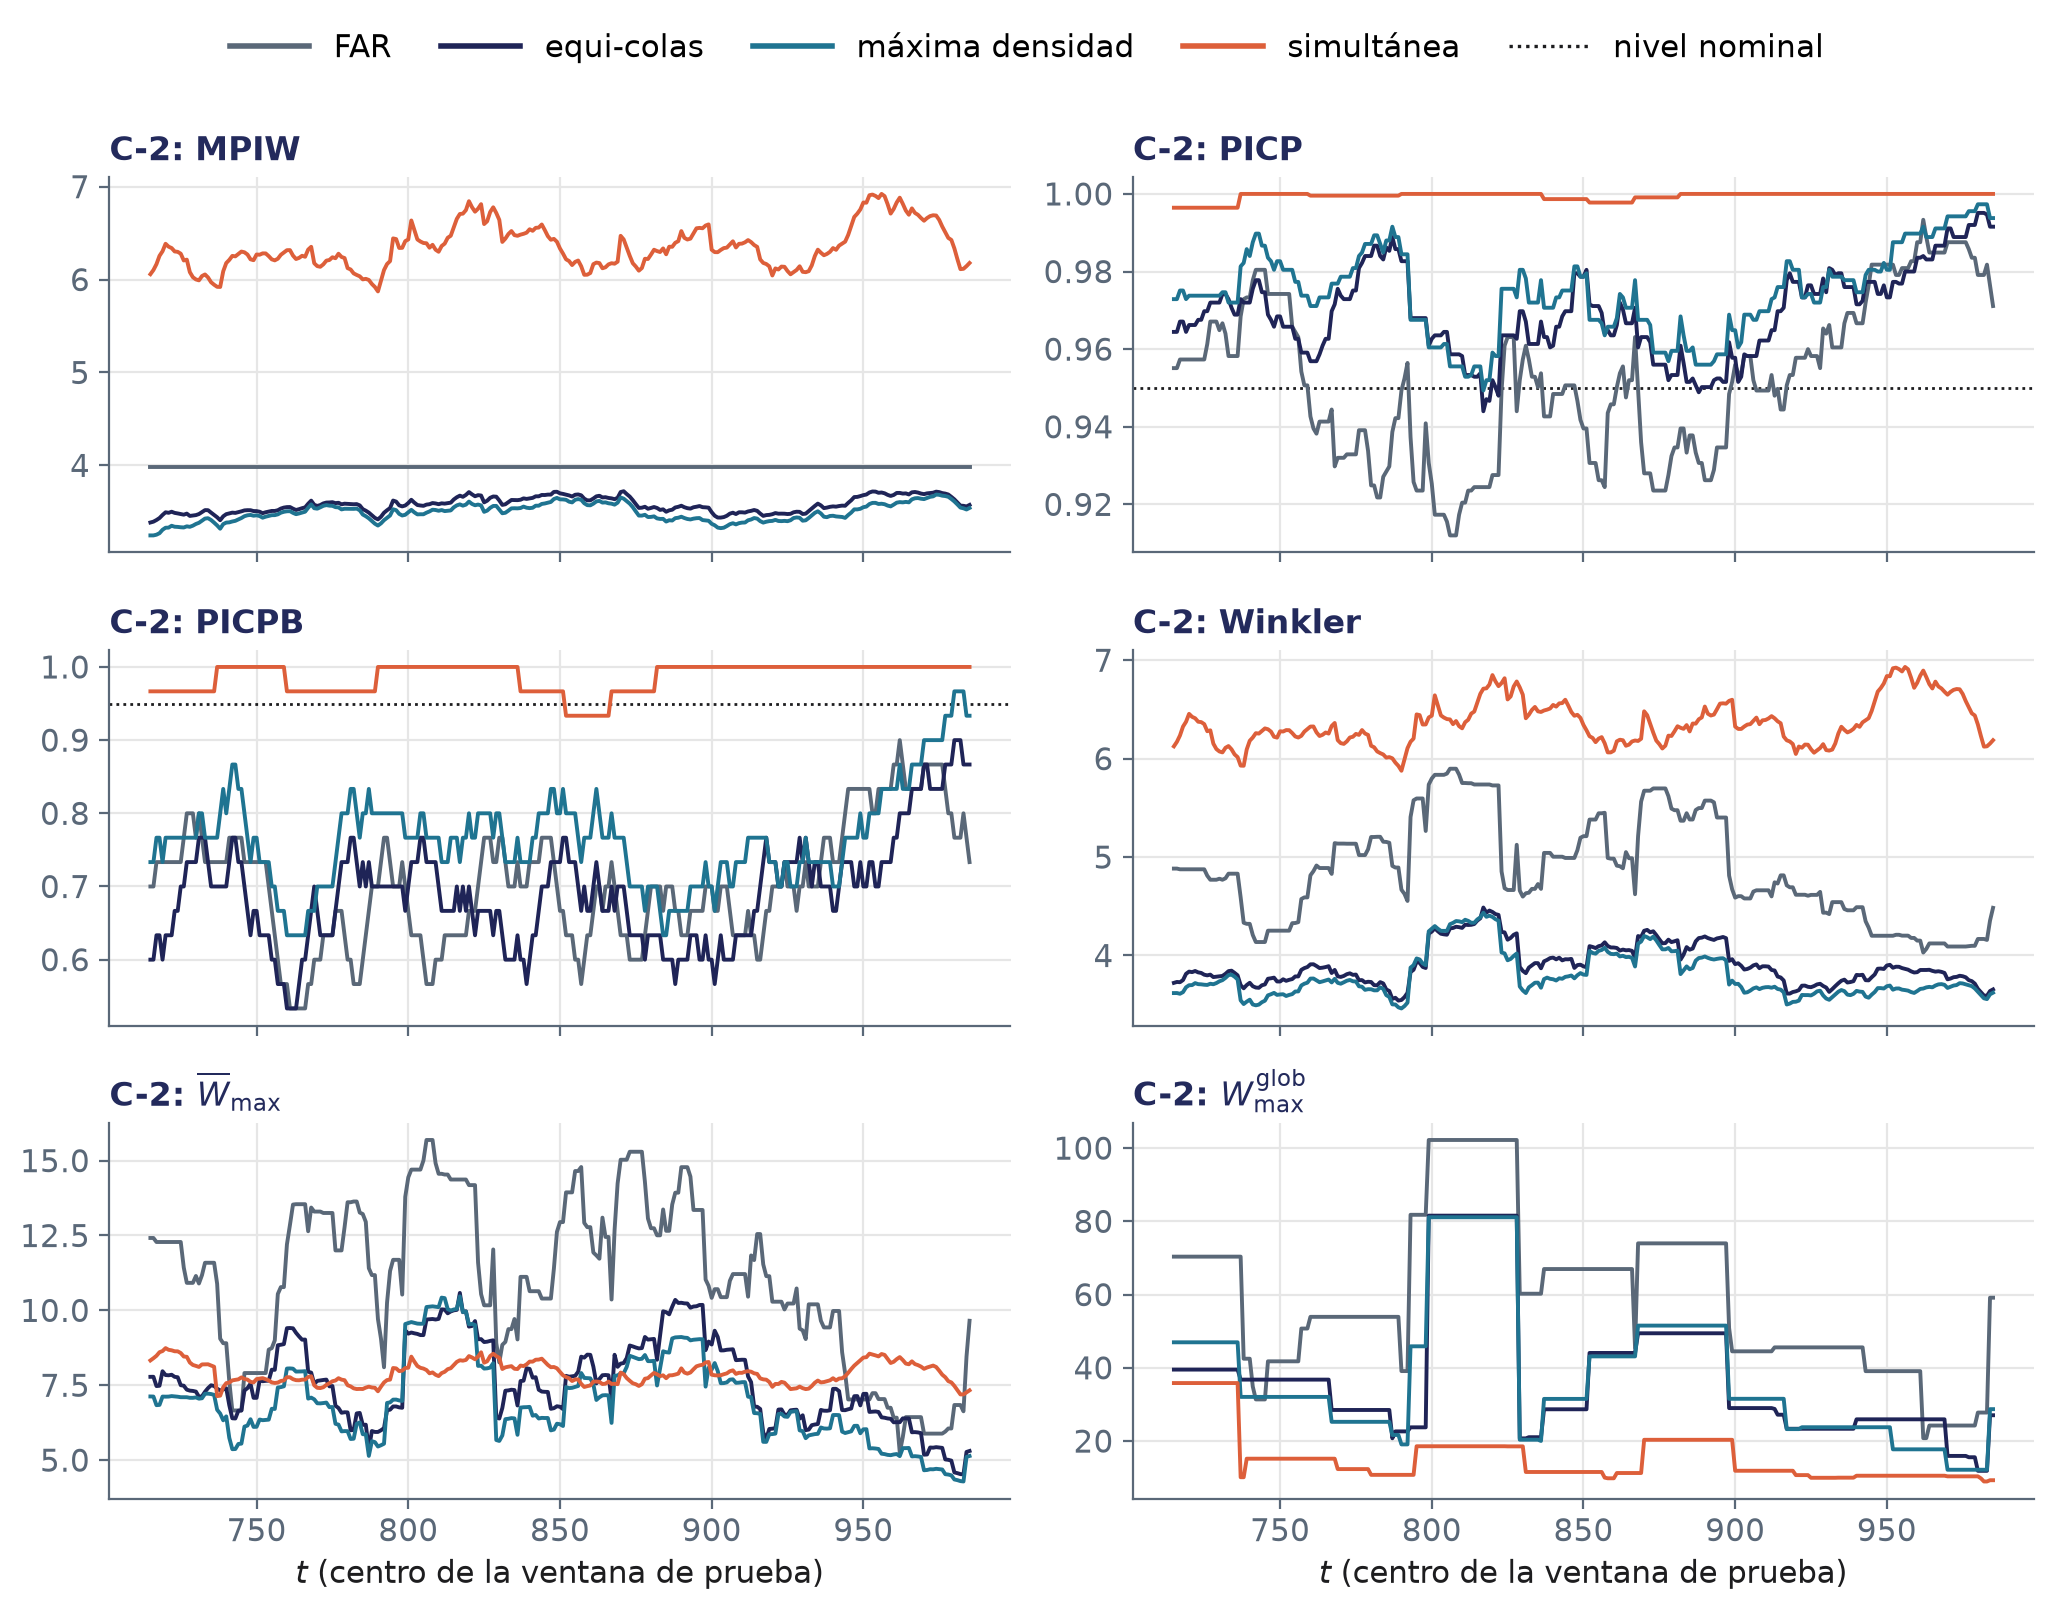
\includegraphics[width=\textwidth,height=0.75\textheight,keepaspectratio]{IMG/aneB_00/aneB_00_ventana_intervalos_w30_C2.png}
\caption{C-2 (TAR). Métricas de intervalo sobre la ventana móvil ($M_{\mathrm{ref}}$).}
\label{fig:aneB_int_C2}
\end{figure}

\begin{figure}[H]
\centering
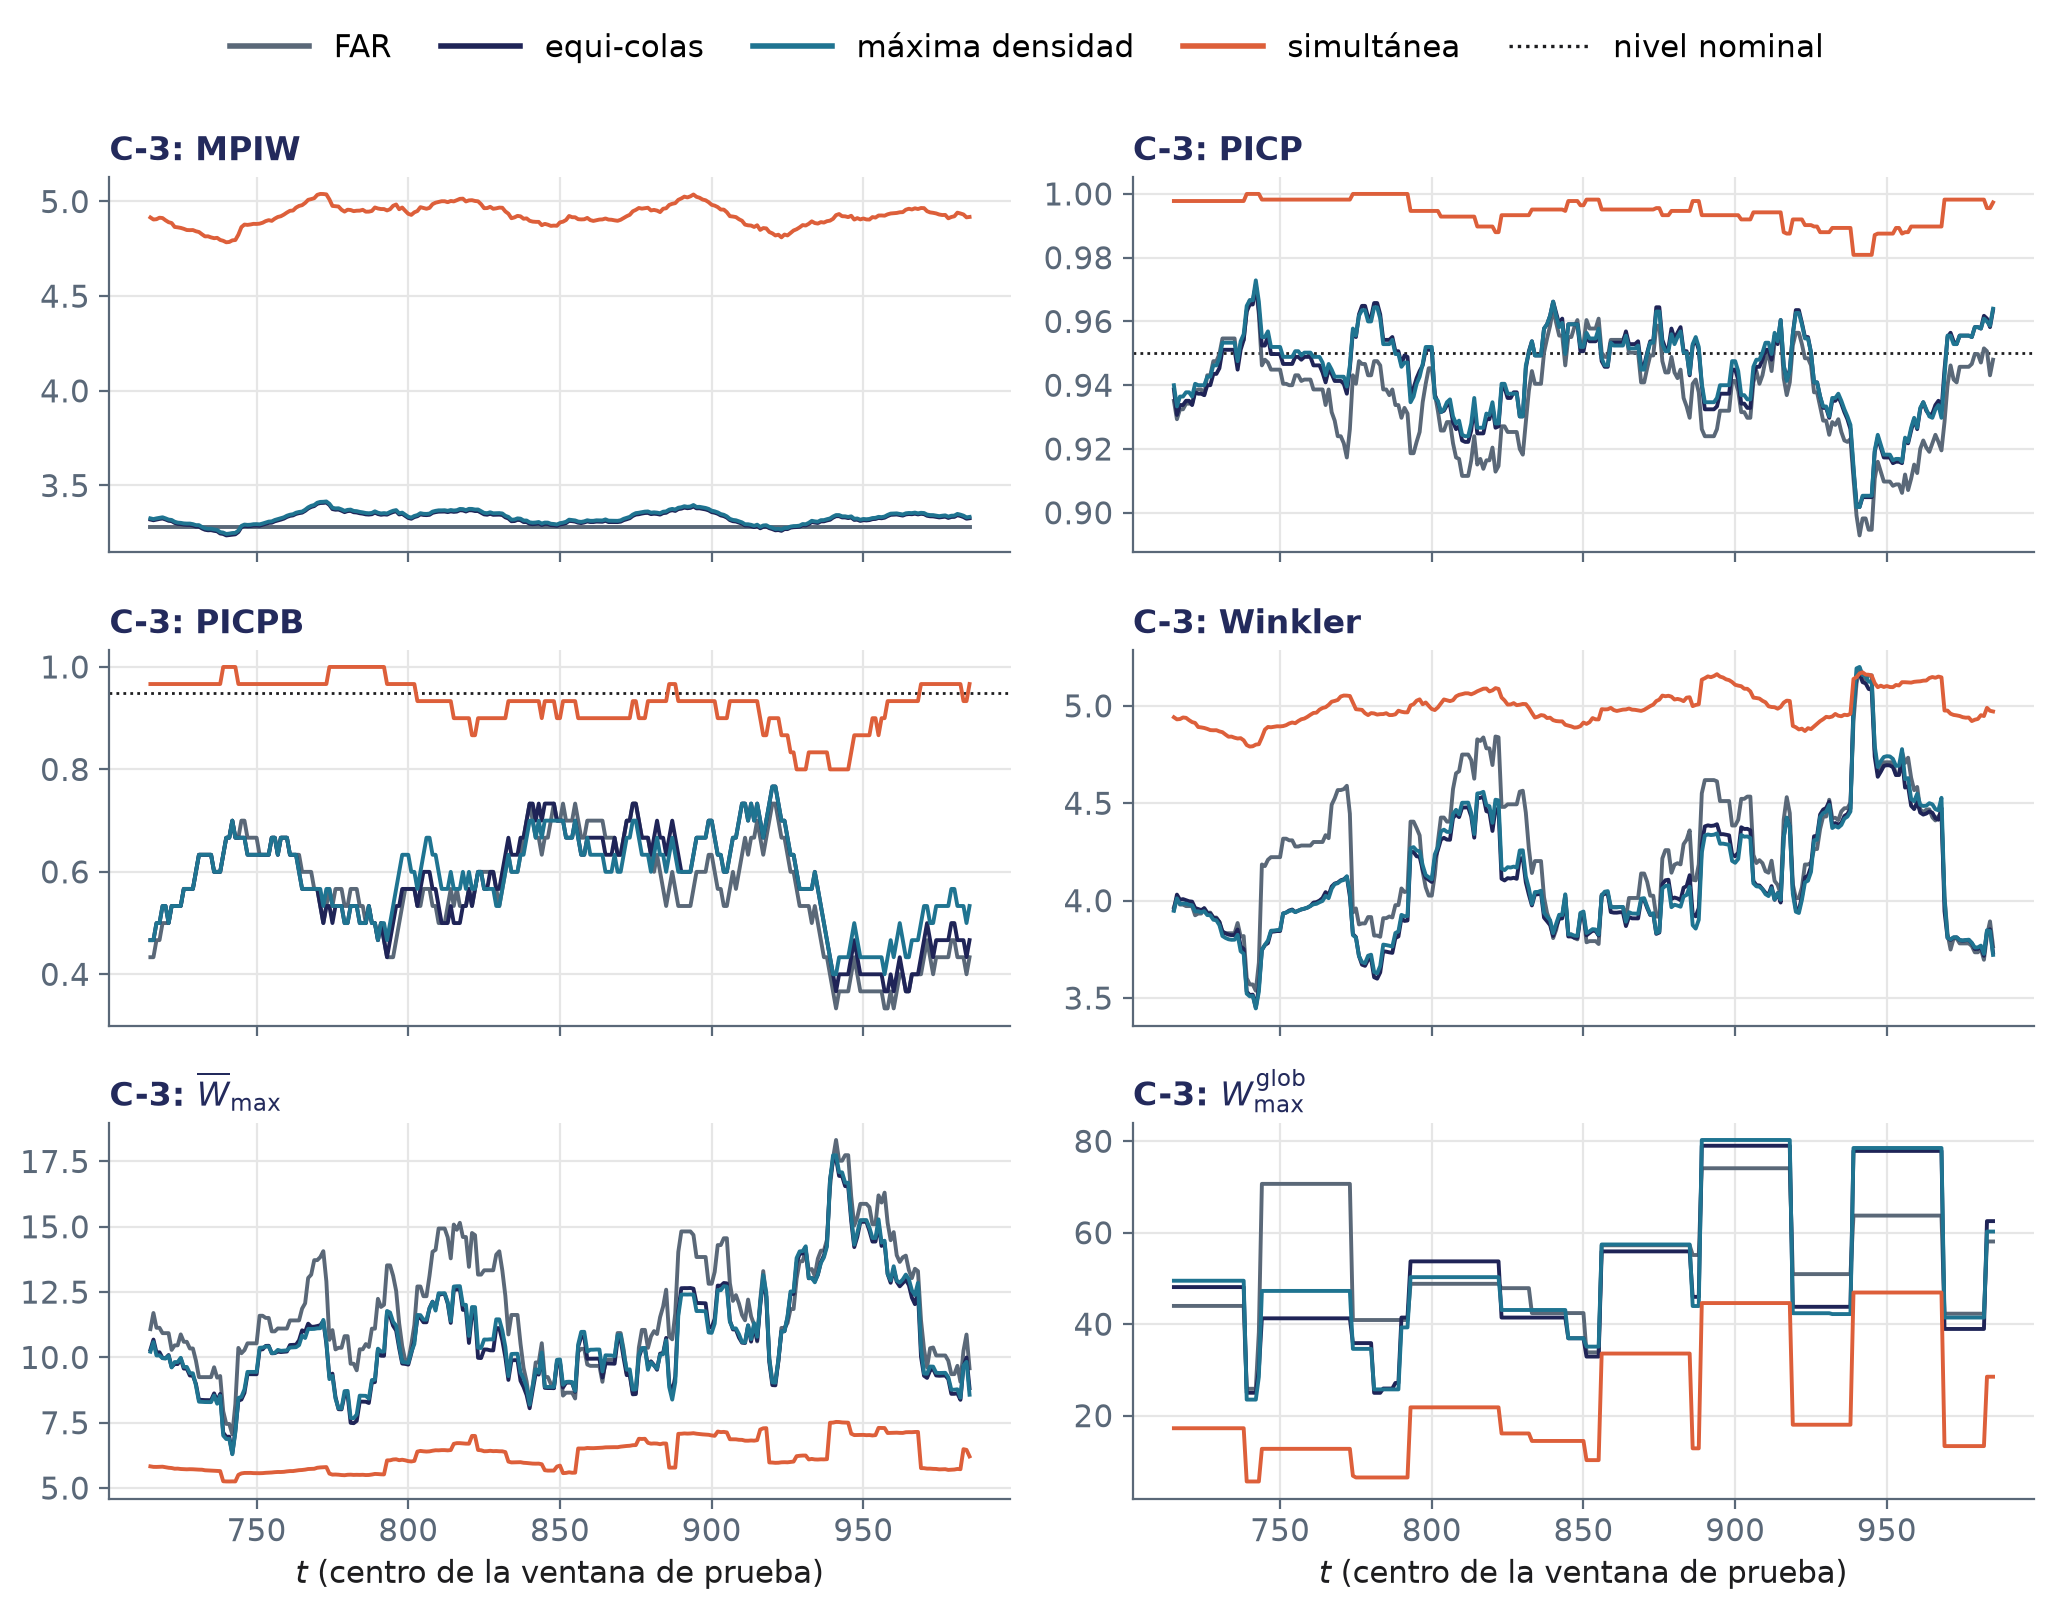
\includegraphics[width=\textwidth,height=0.75\textheight,keepaspectratio]{IMG/aneB_00/aneB_00_ventana_intervalos_w30_C3.png}
\caption{C-3 (multimodalidad). Métricas de intervalo sobre la ventana móvil ($M_{\mathrm{ref}}$).}
\label{fig:aneB_int_C3}
\end{figure}

\section{Calibración respecto de la representación truncada}
\label{aneB_00_04_calibracion_truncada}

Las métricas evaluadas contra la representación $X_t^{(M)}$ en lugar de la curva suavizada, en función de $M$.

\begin{figure}[H]
\centering
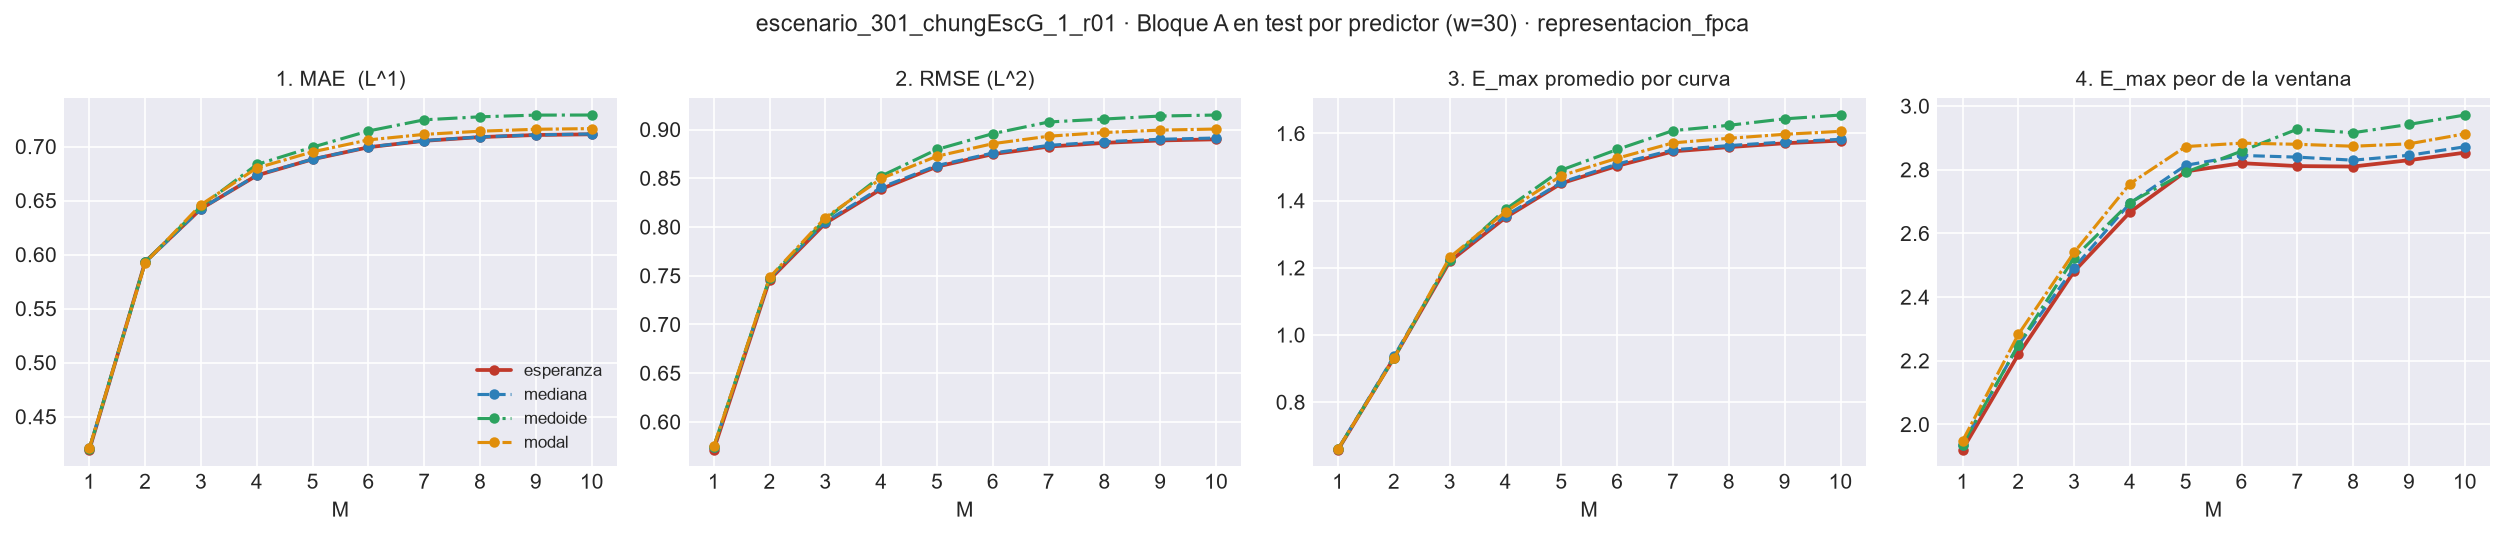
\includegraphics[width=\textwidth,height=0.4\textheight,keepaspectratio]{IMG/aneB_00/aneB_00_bloqueA_vs_M_repr_C1.png}
\caption{C-1 (GARCH). Métricas de error contra la representación truncada, por $M$.}
\label{fig:aneB_reprA_C1}
\end{figure}

\begin{figure}[H]
\centering
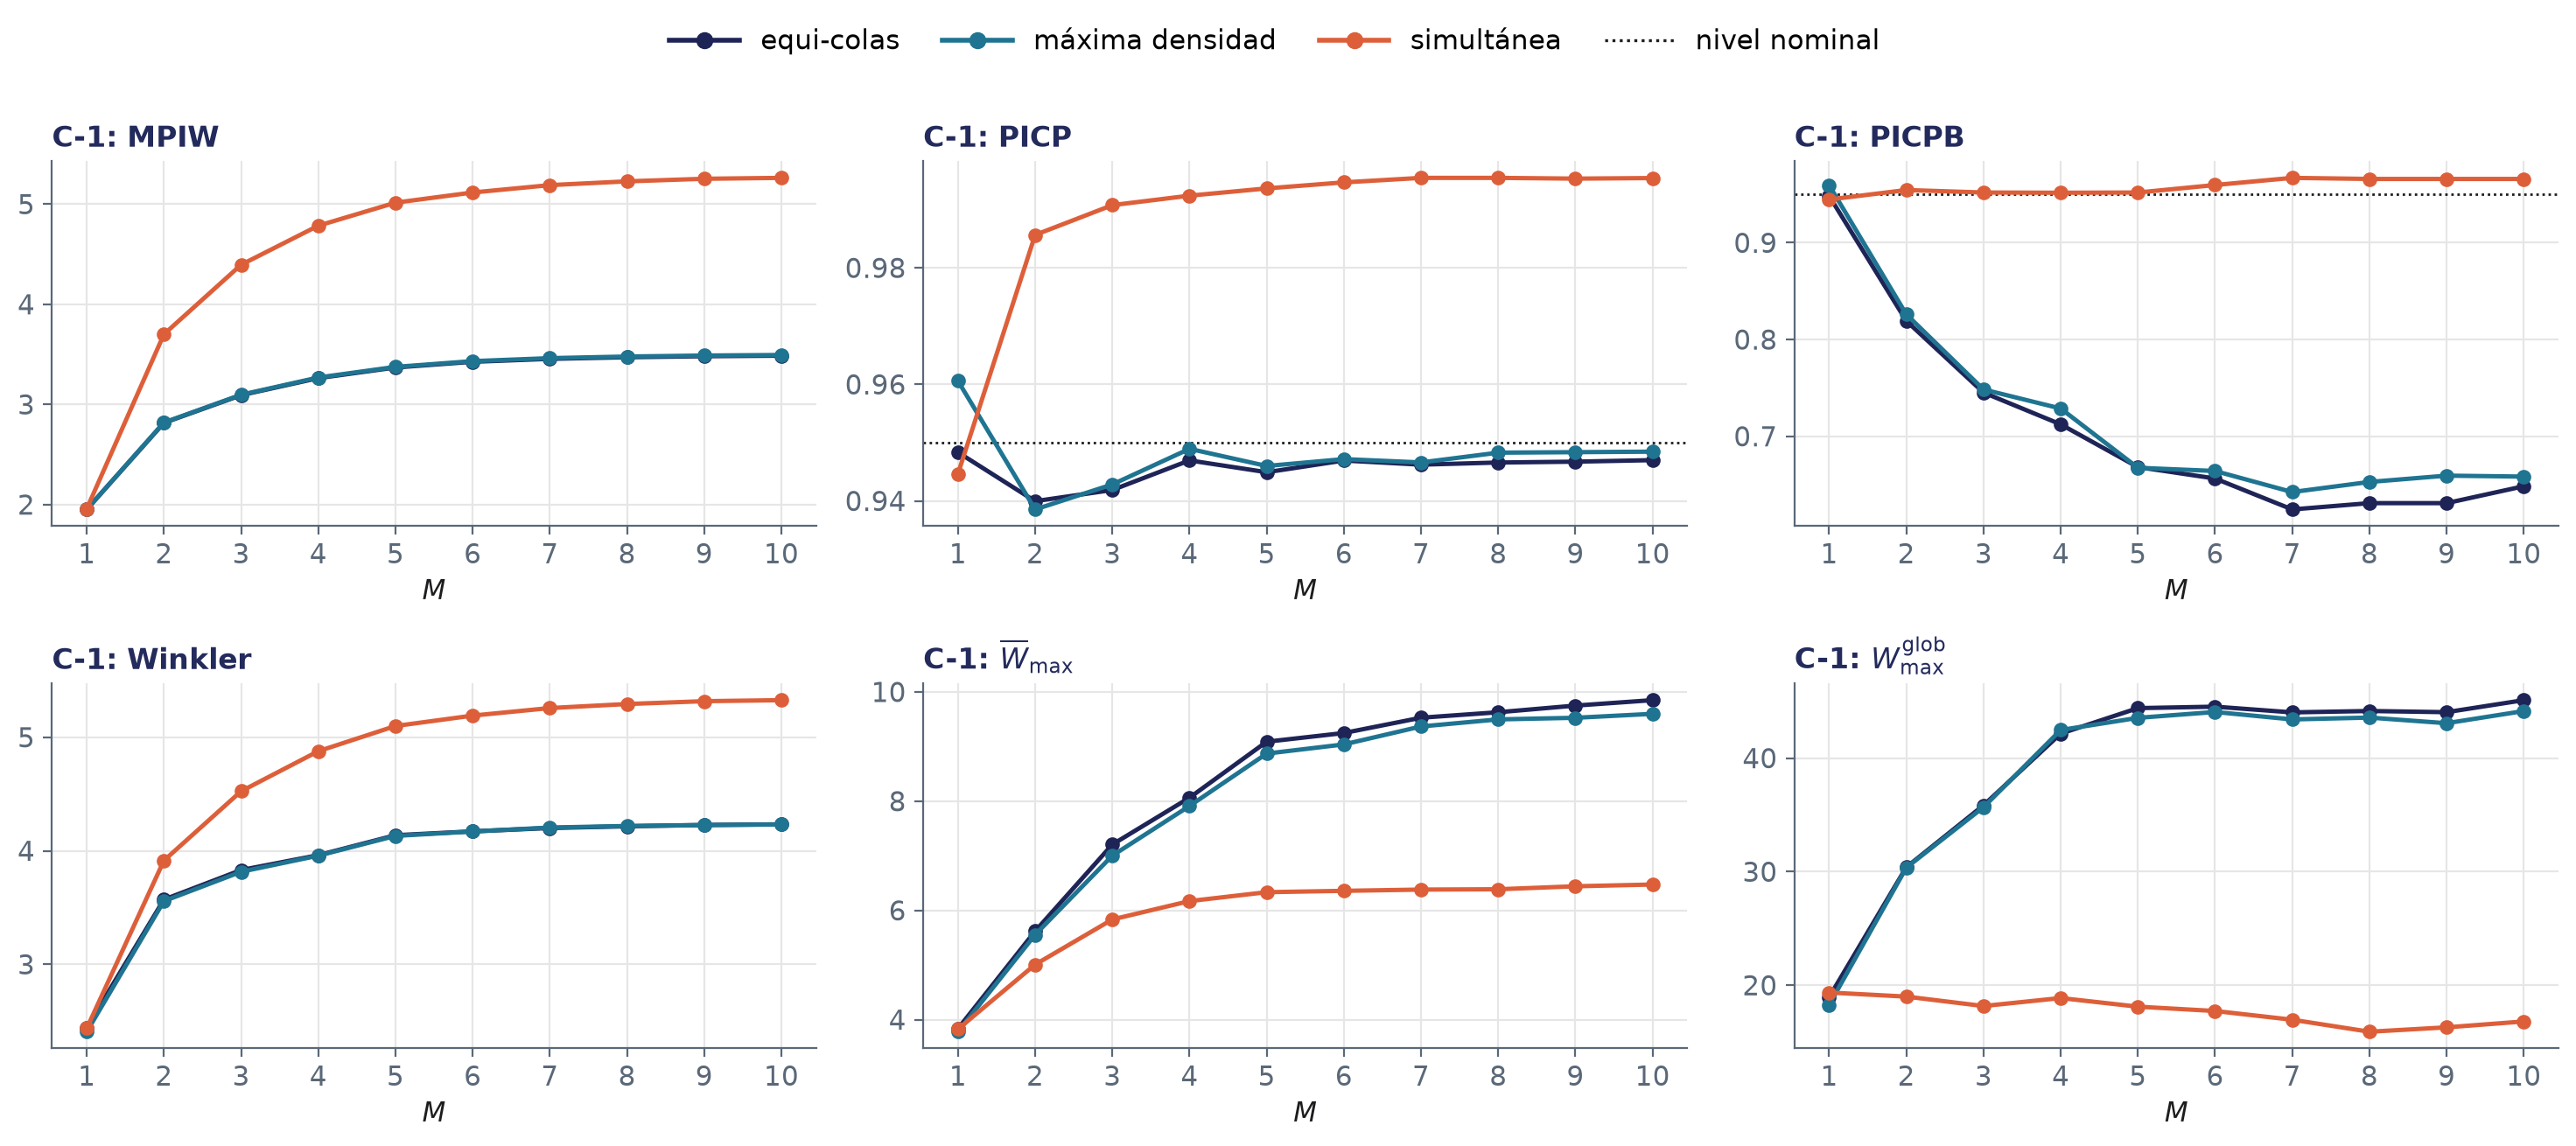
\includegraphics[width=\textwidth,height=0.4\textheight,keepaspectratio]{IMG/aneB_00/aneB_00_bloqueB_vs_M_repr_C1.png}
\caption{C-1 (GARCH). Métricas de intervalo contra la representación truncada, por $M$.}
\label{fig:aneB_reprB_C1}
\end{figure}

\begin{figure}[H]
\centering
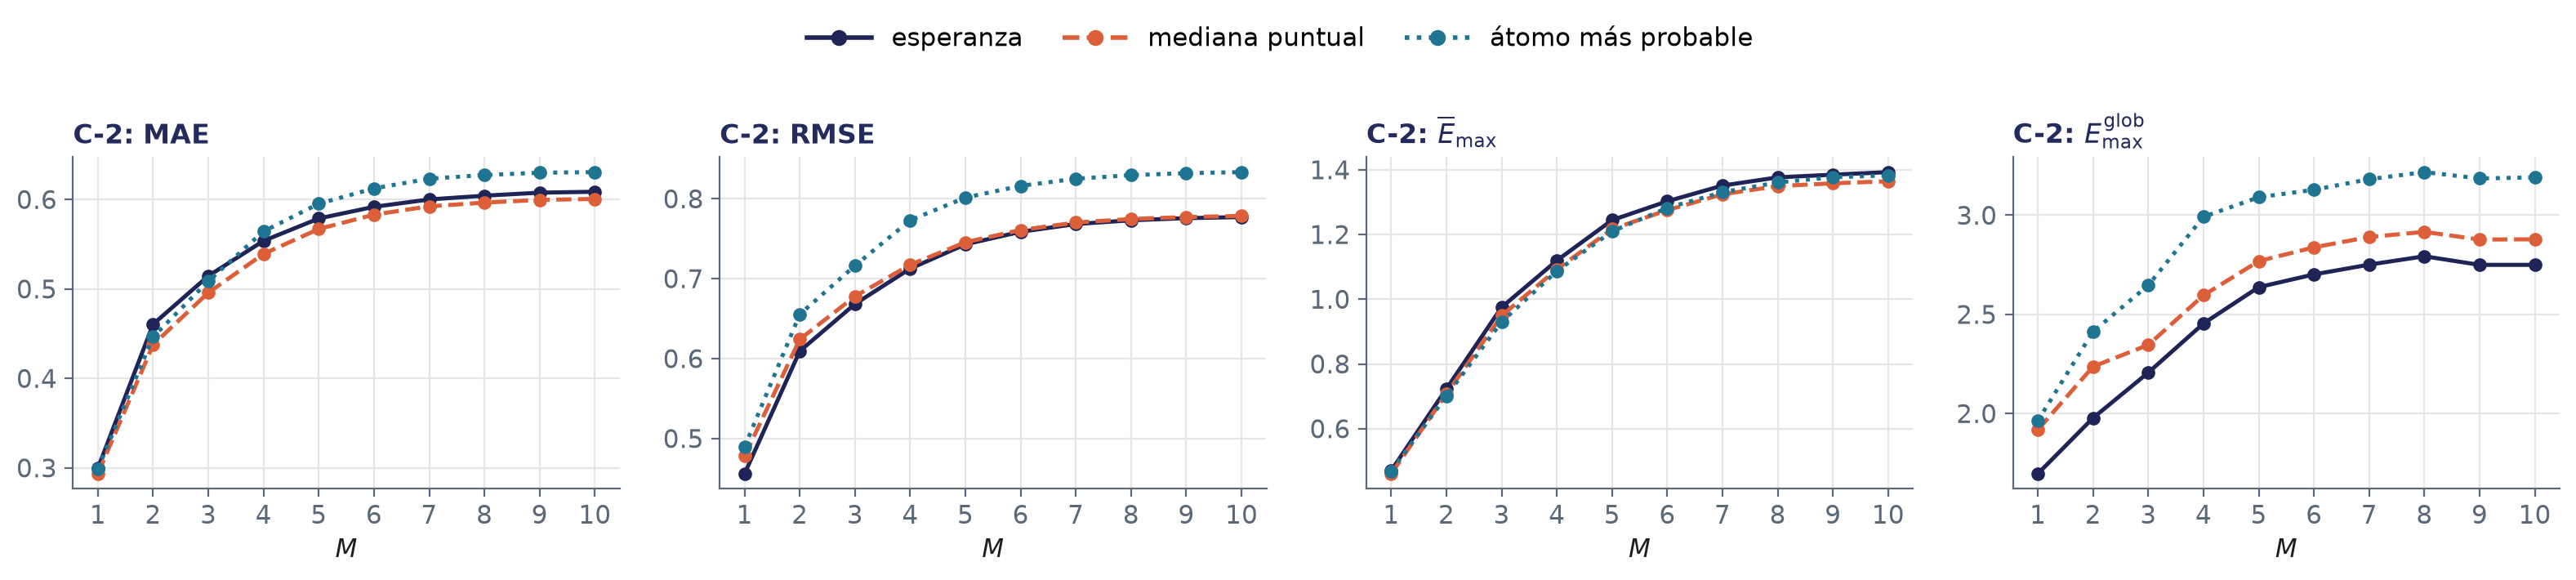
\includegraphics[width=\textwidth,height=0.4\textheight,keepaspectratio]{IMG/aneB_00/aneB_00_bloqueA_vs_M_repr_C2.png}
\caption{C-2 (TAR). Métricas de error contra la representación truncada, por $M$.}
\label{fig:aneB_reprA_C2}
\end{figure}

\begin{figure}[H]
\centering
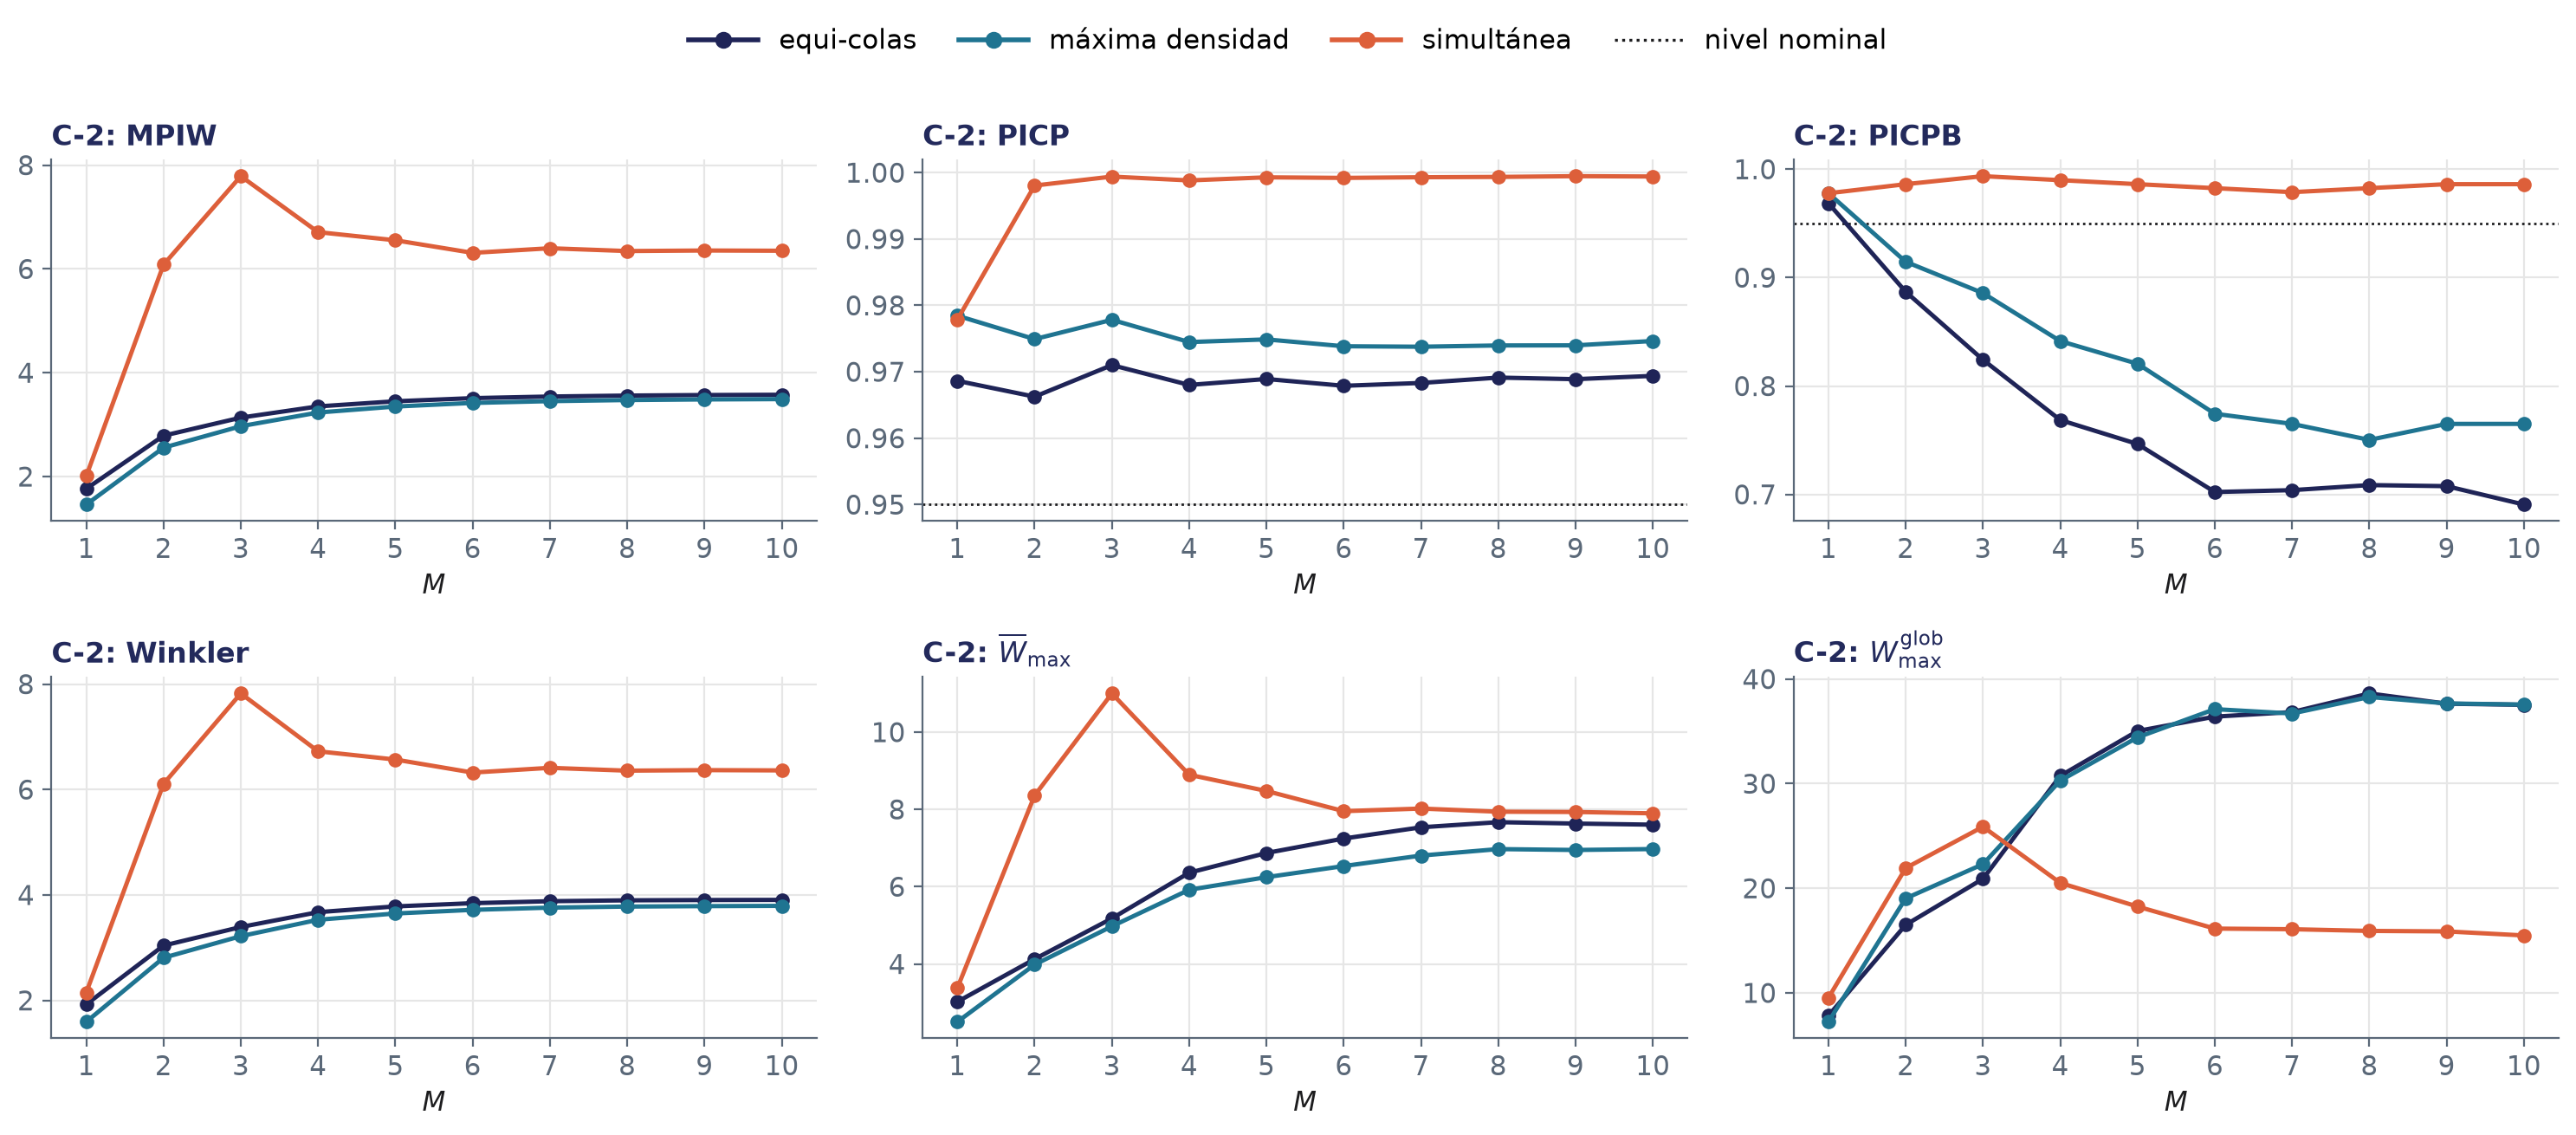
\includegraphics[width=\textwidth,height=0.4\textheight,keepaspectratio]{IMG/aneB_00/aneB_00_bloqueB_vs_M_repr_C2.png}
\caption{C-2 (TAR). Métricas de intervalo contra la representación truncada, por $M$.}
\label{fig:aneB_reprB_C2}
\end{figure}

\begin{figure}[H]
\centering
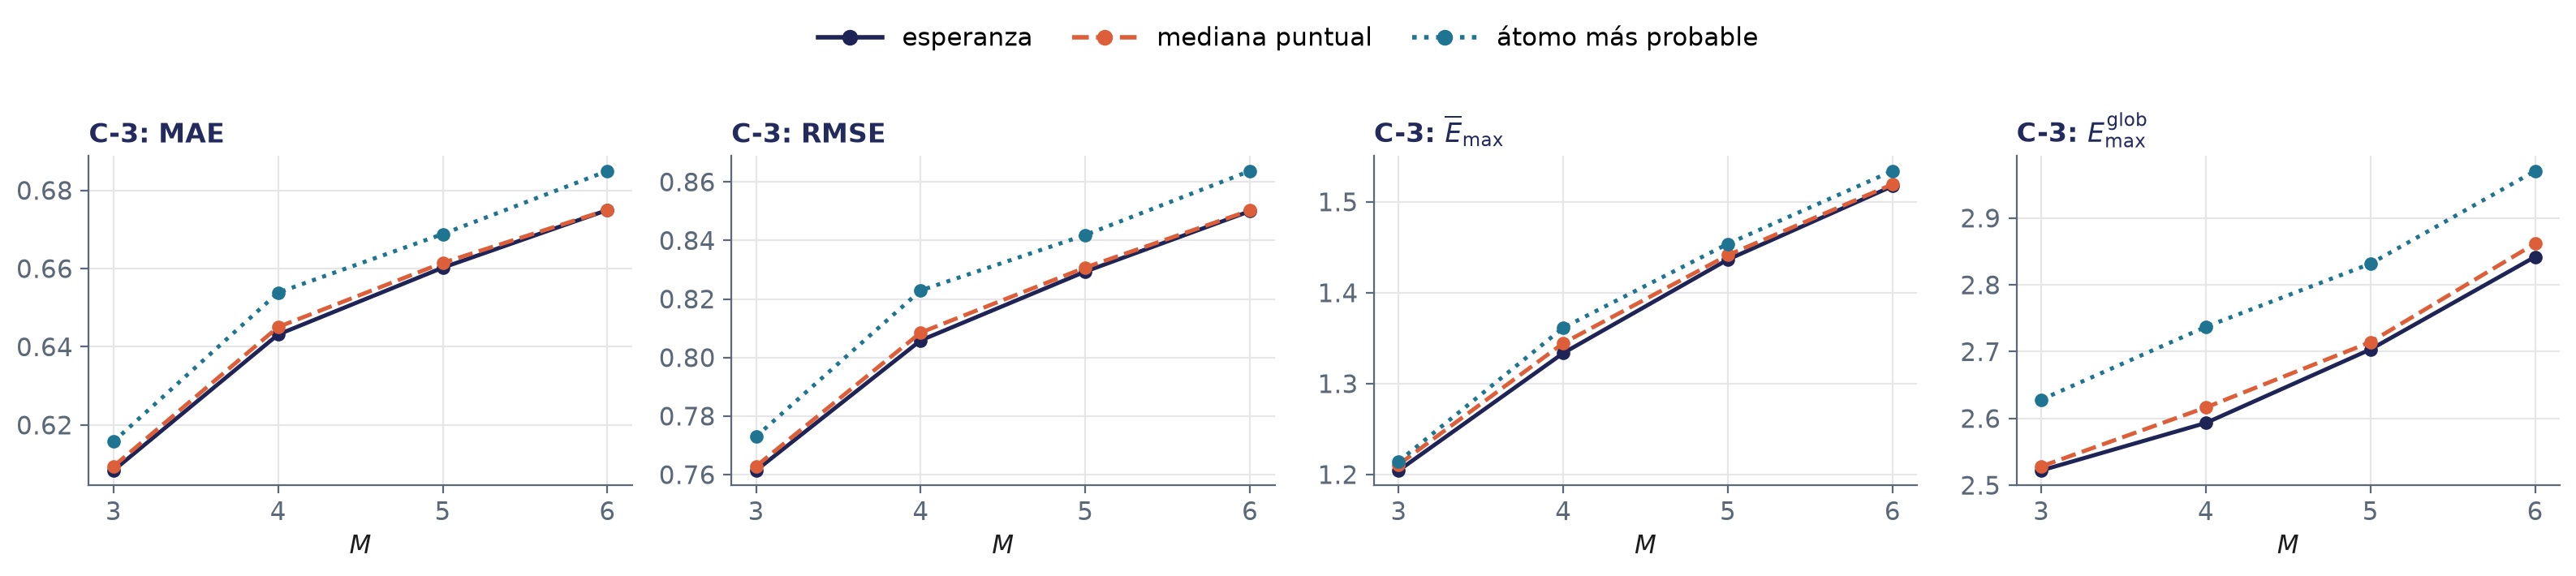
\includegraphics[width=\textwidth,height=0.4\textheight,keepaspectratio]{IMG/aneB_00/aneB_00_bloqueA_vs_M_repr_C3.png}
\caption{C-3 (multimodalidad). Métricas de error contra la representación truncada, por $M$.}
\label{fig:aneB_reprA_C3}
\end{figure}

\begin{figure}[H]
\centering
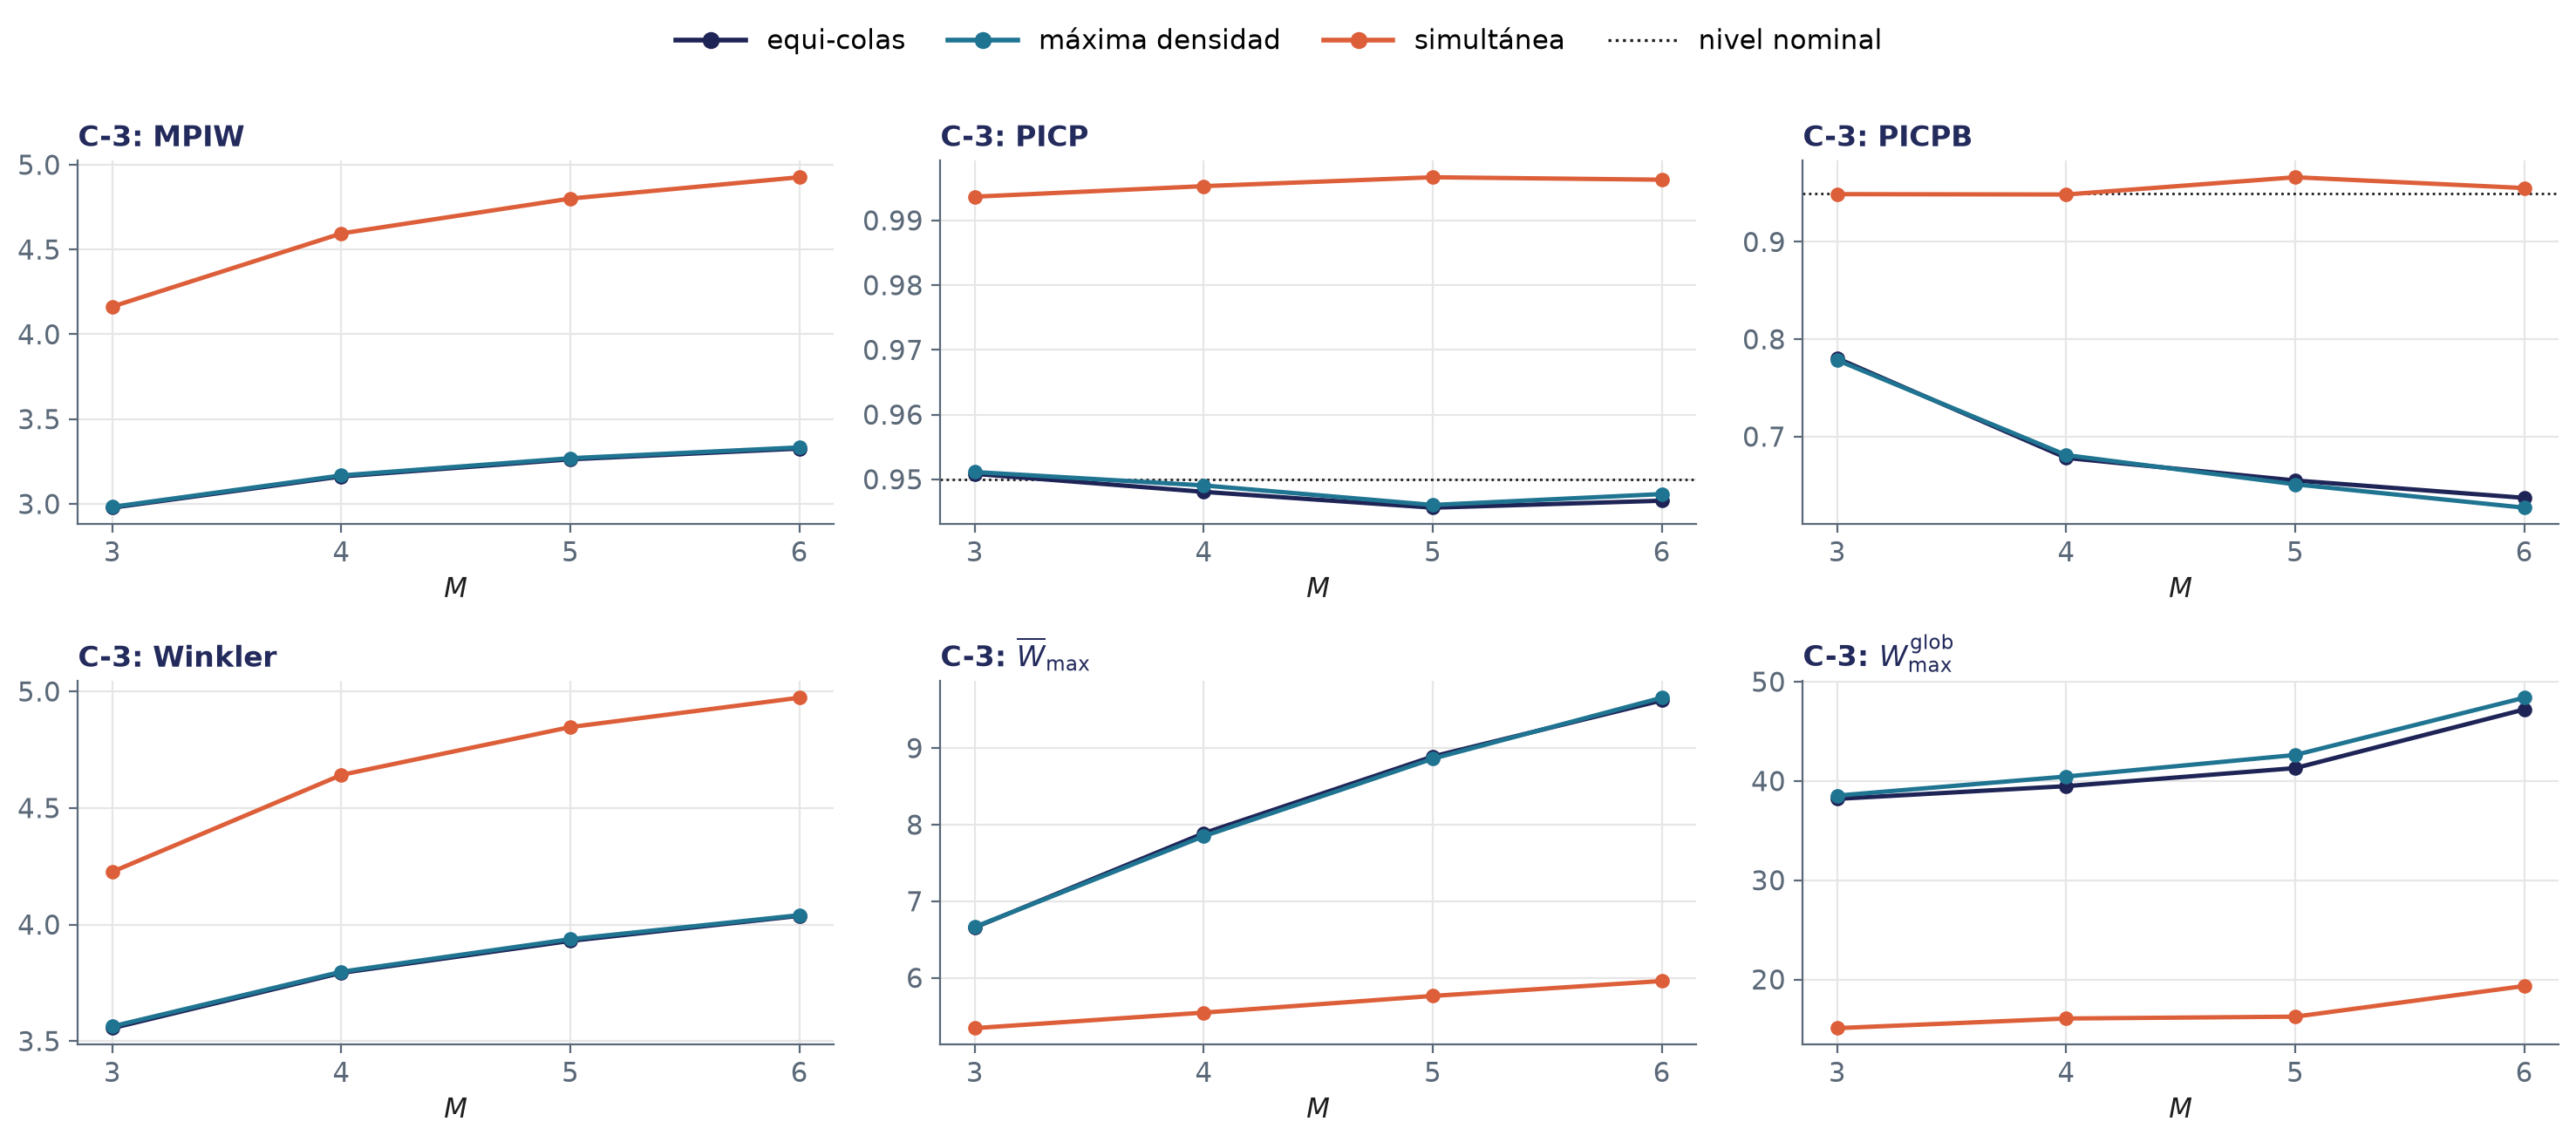
\includegraphics[width=\textwidth,height=0.4\textheight,keepaspectratio]{IMG/aneB_00/aneB_00_bloqueB_vs_M_repr_C3.png}
\caption{C-3 (multimodalidad). Métricas de intervalo contra la representación truncada, por $M$.}
\label{fig:aneB_reprB_C3}
\end{figure}

\section{Intervalos por componente}
\label{aneB_00_05_intervalos_componente}

Banda de credibilidad al 95\% de cada score y dispersión estimada frente a la observada.

\begin{figure}[H]
\centering
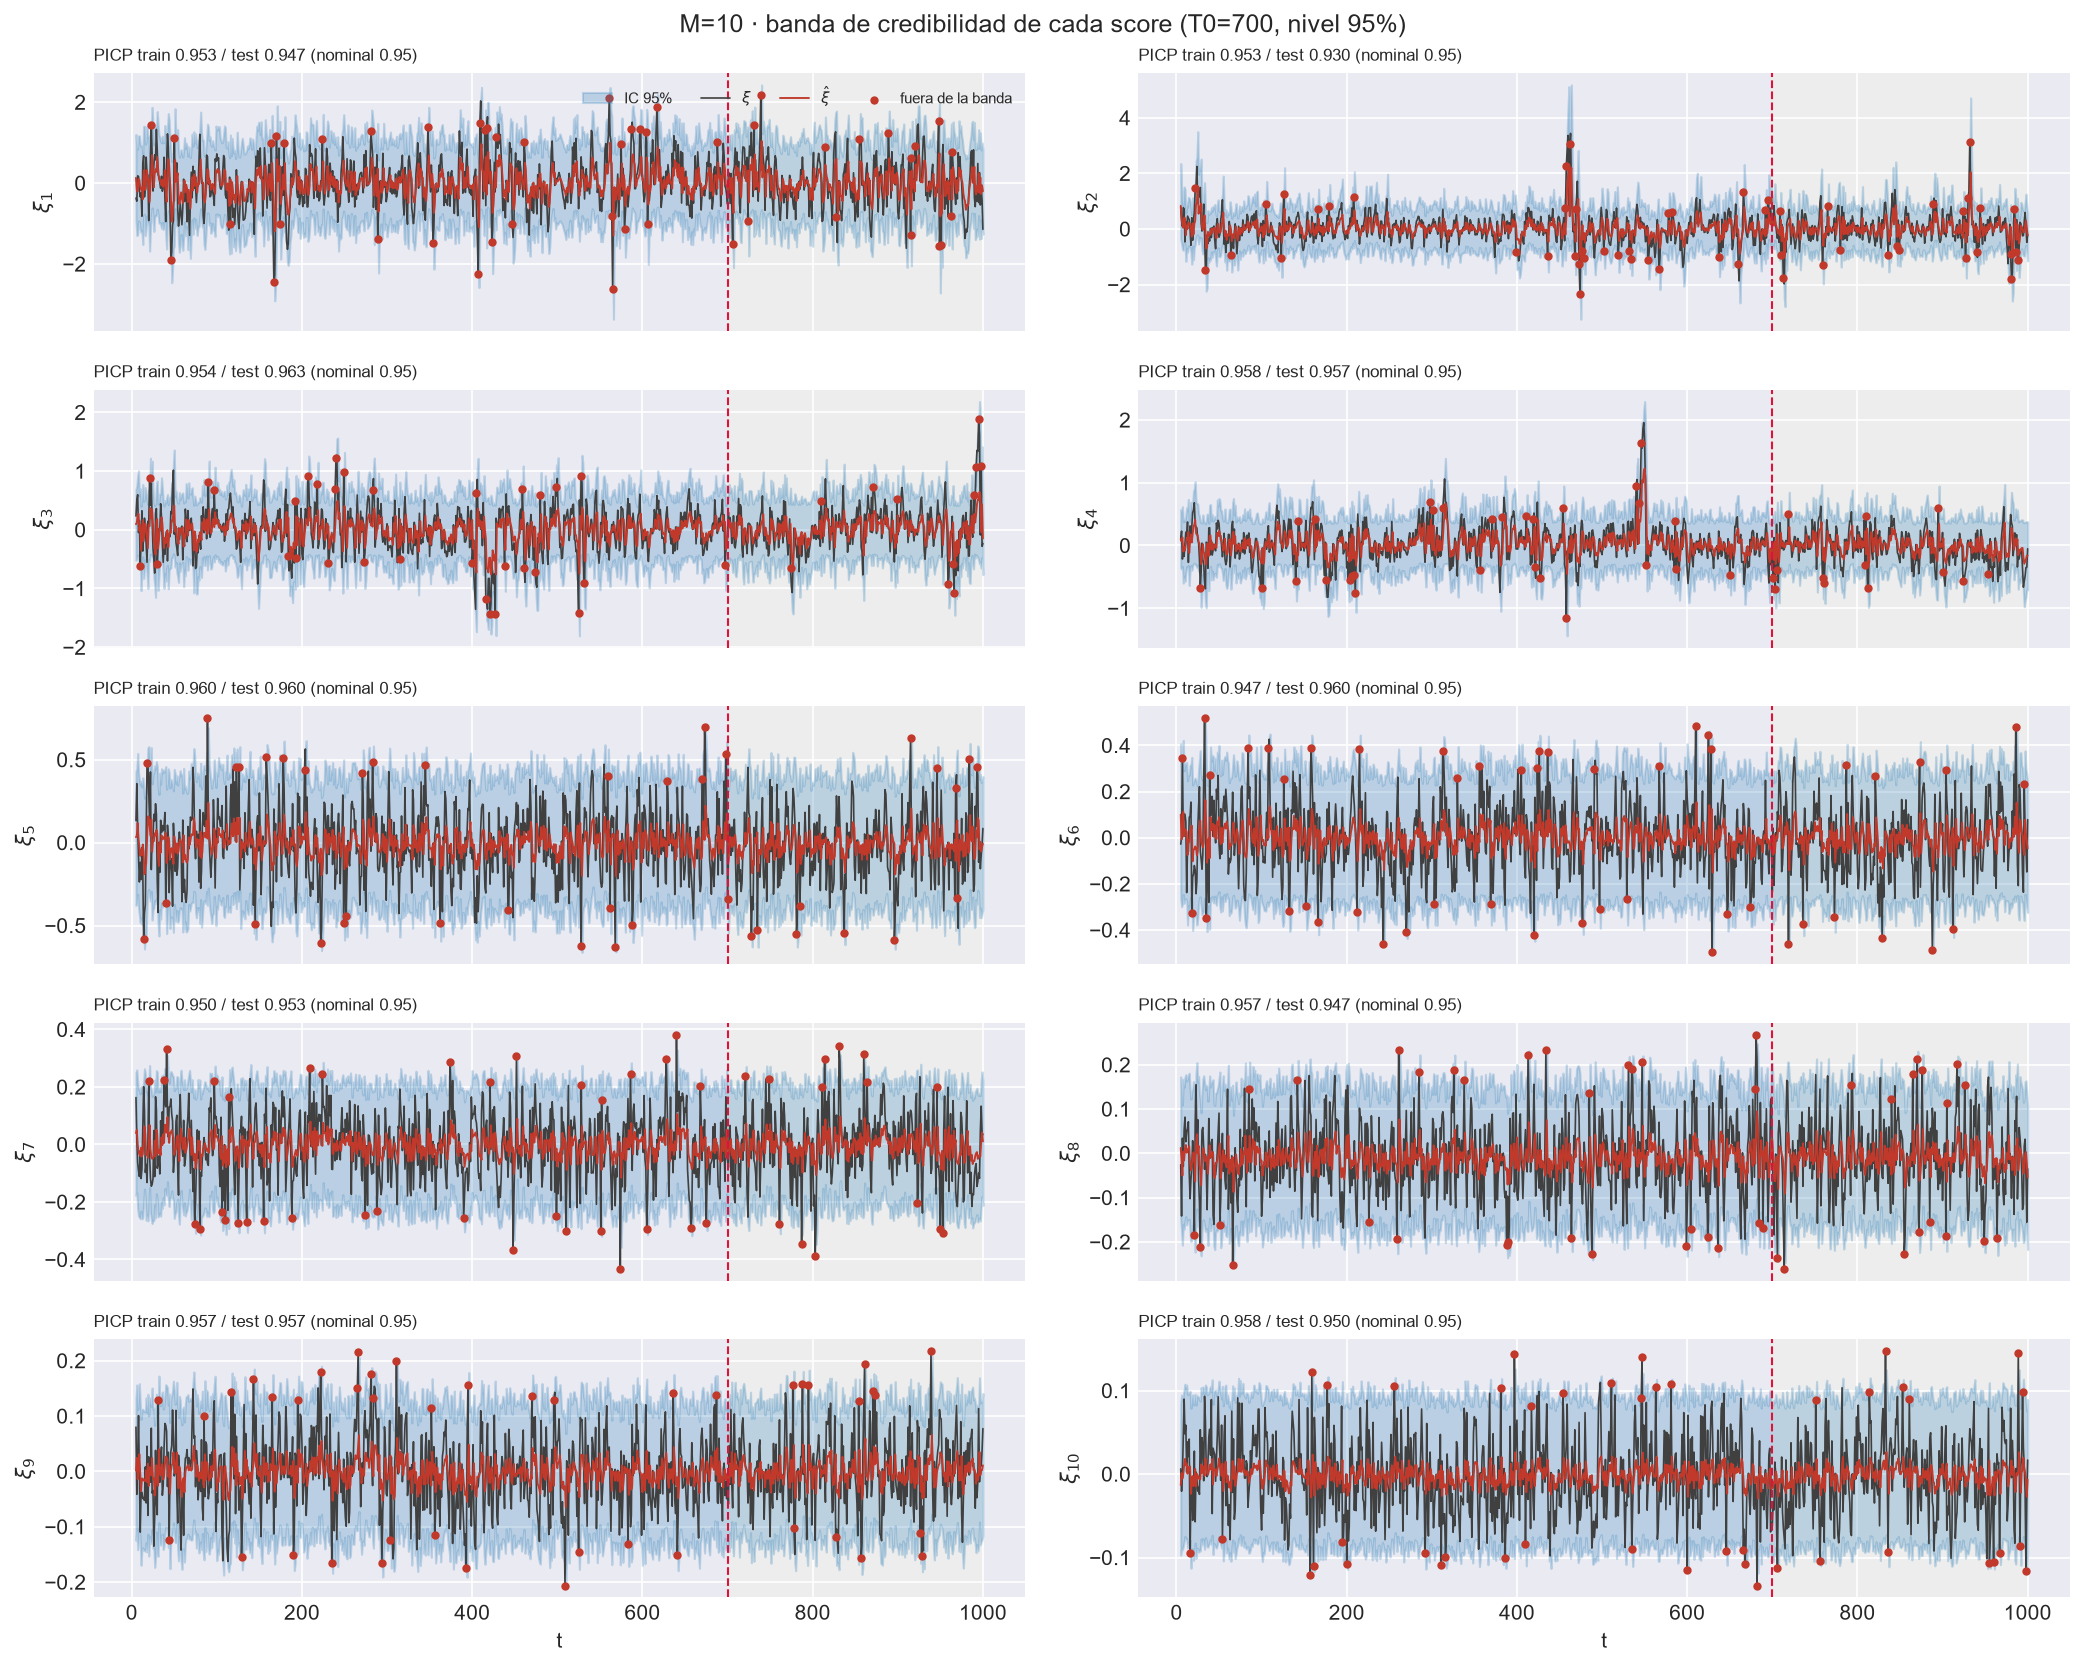
\includegraphics[width=\textwidth,height=0.7\textheight,keepaspectratio]{IMG/aneB_00/aneB_00_scores_banda_C1.png}
\caption{C-1 (GARCH). Banda de credibilidad de cada score ($M_{\mathrm{ref}}$).}
\label{fig:aneB_banda_C1}
\end{figure}

\begin{figure}[H]
\centering
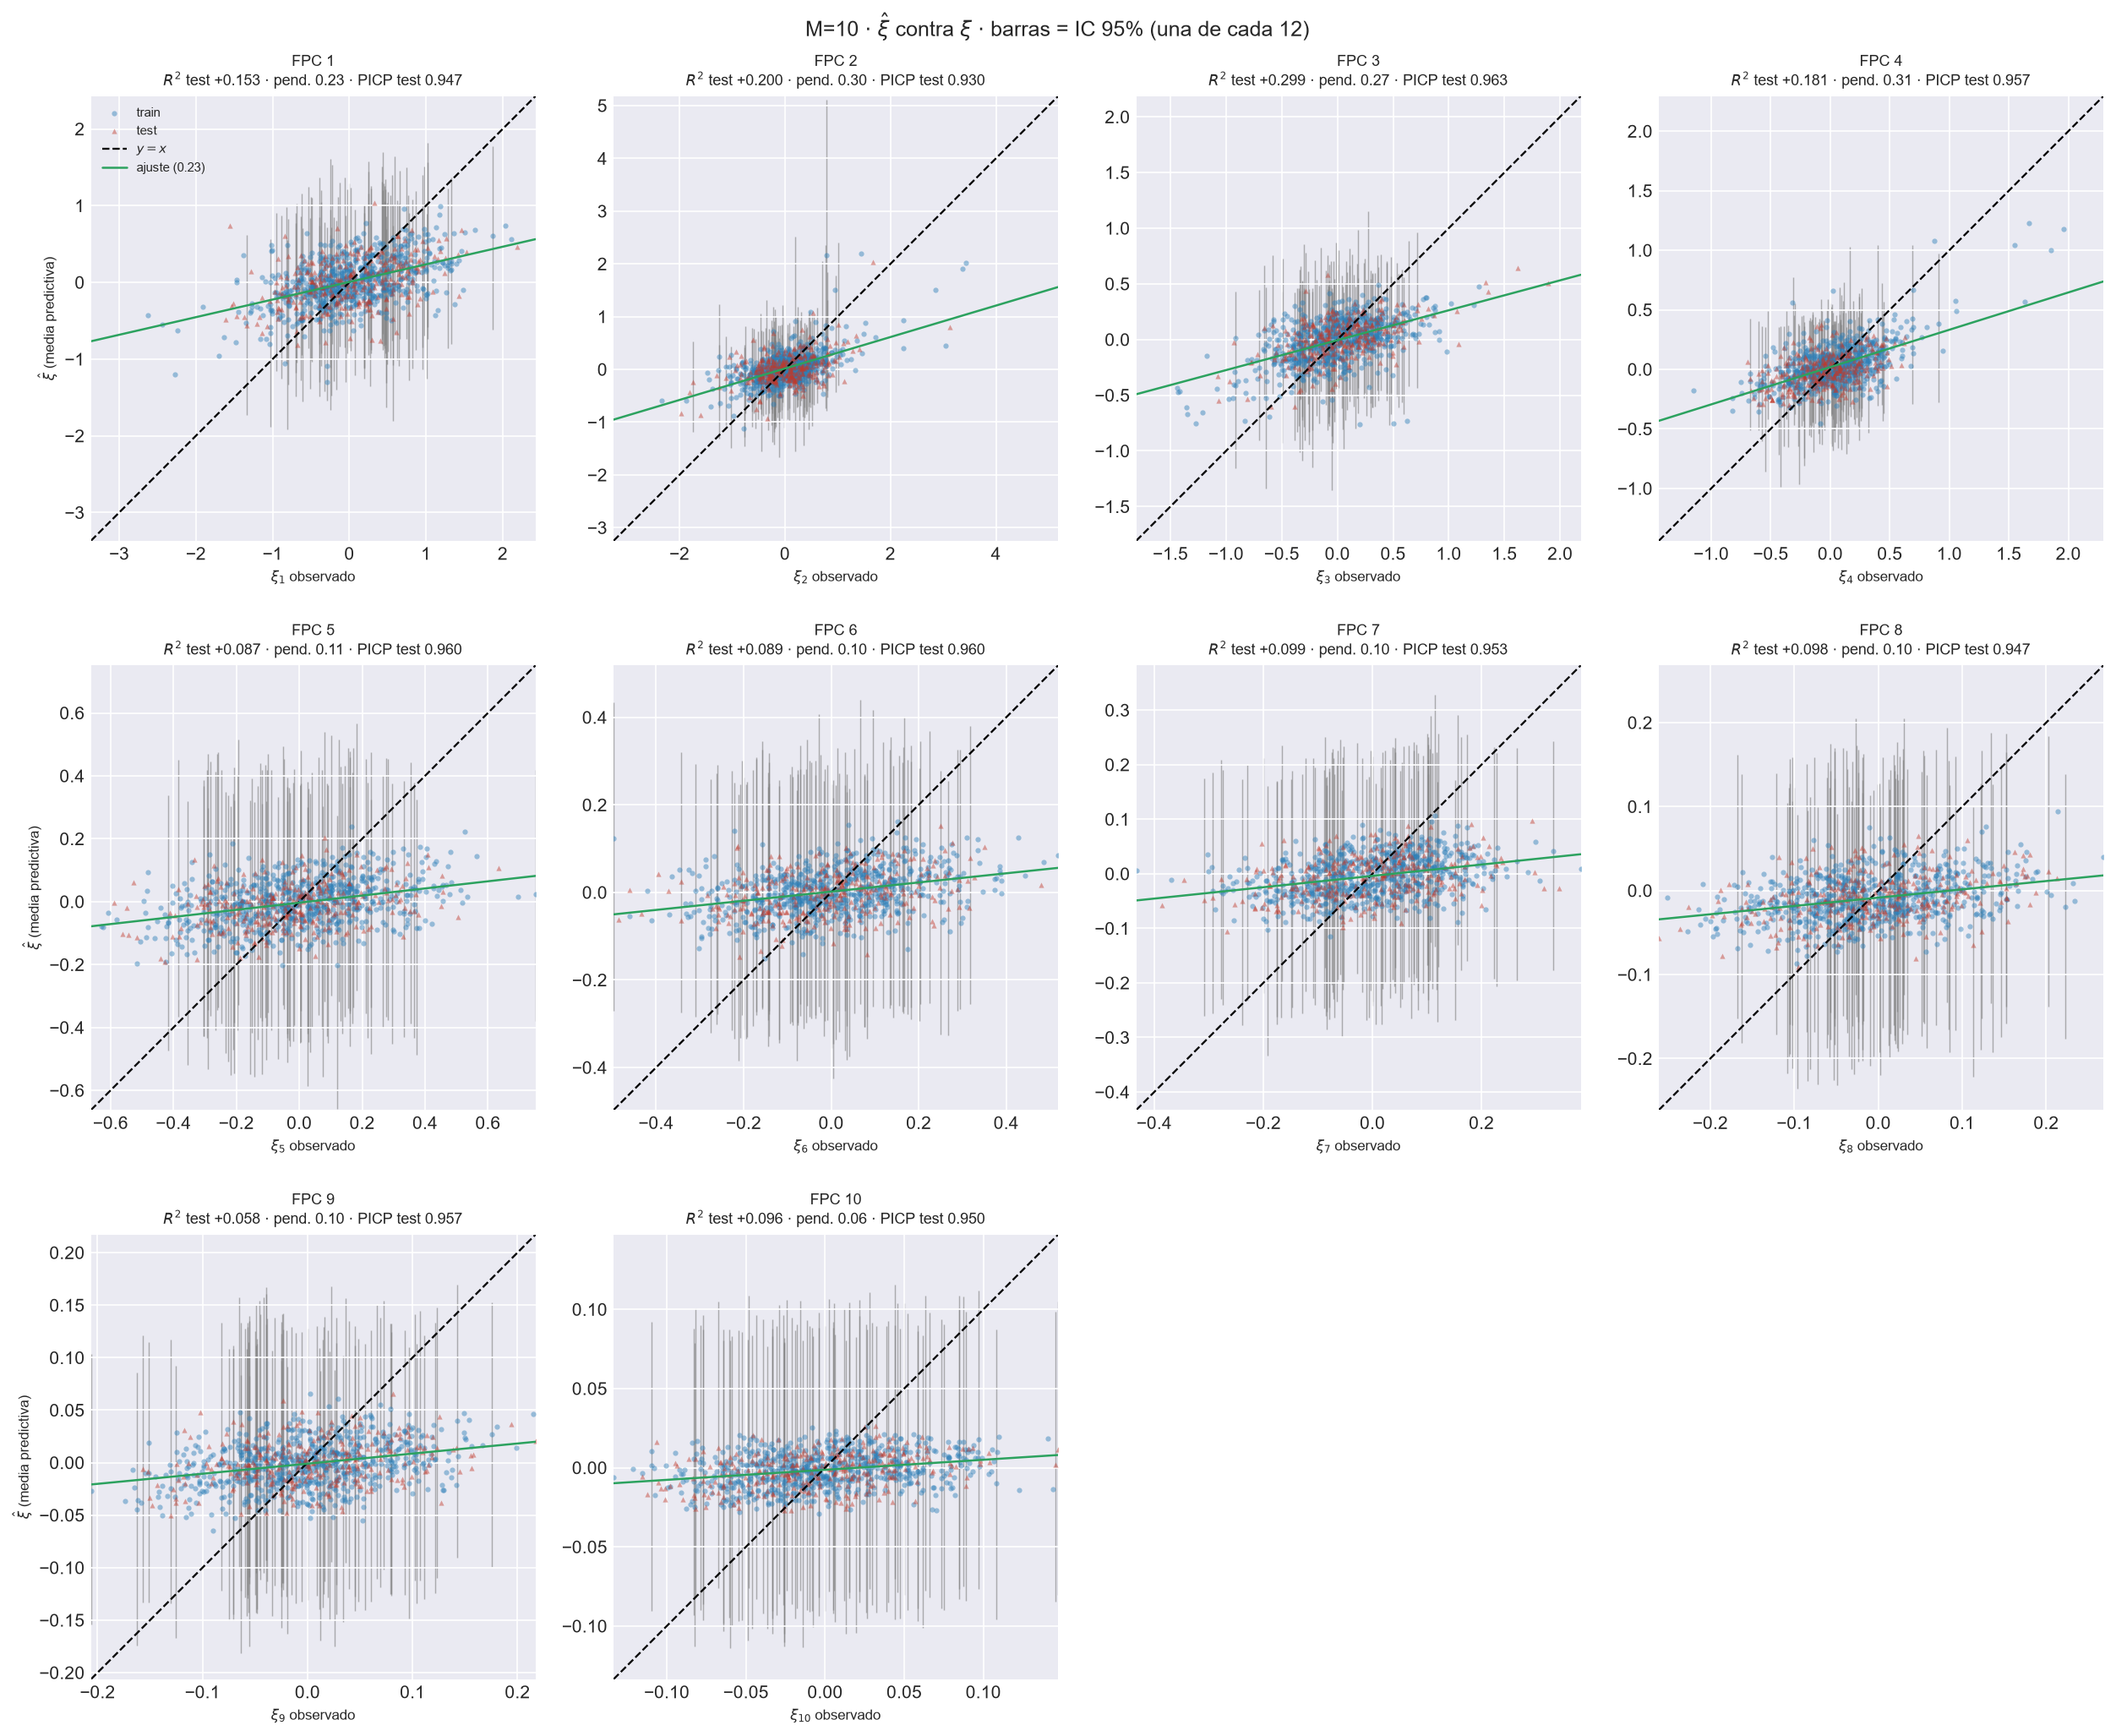
\includegraphics[width=\textwidth,height=0.7\textheight,keepaspectratio]{IMG/aneB_00/aneB_00_scores_dispersion_C1.png}
\caption{C-1 (GARCH). Dispersión estimada de cada score frente a la observada ($M_{\mathrm{ref}}$).}
\label{fig:aneB_disp_C1}
\end{figure}

\begin{figure}[H]
\centering
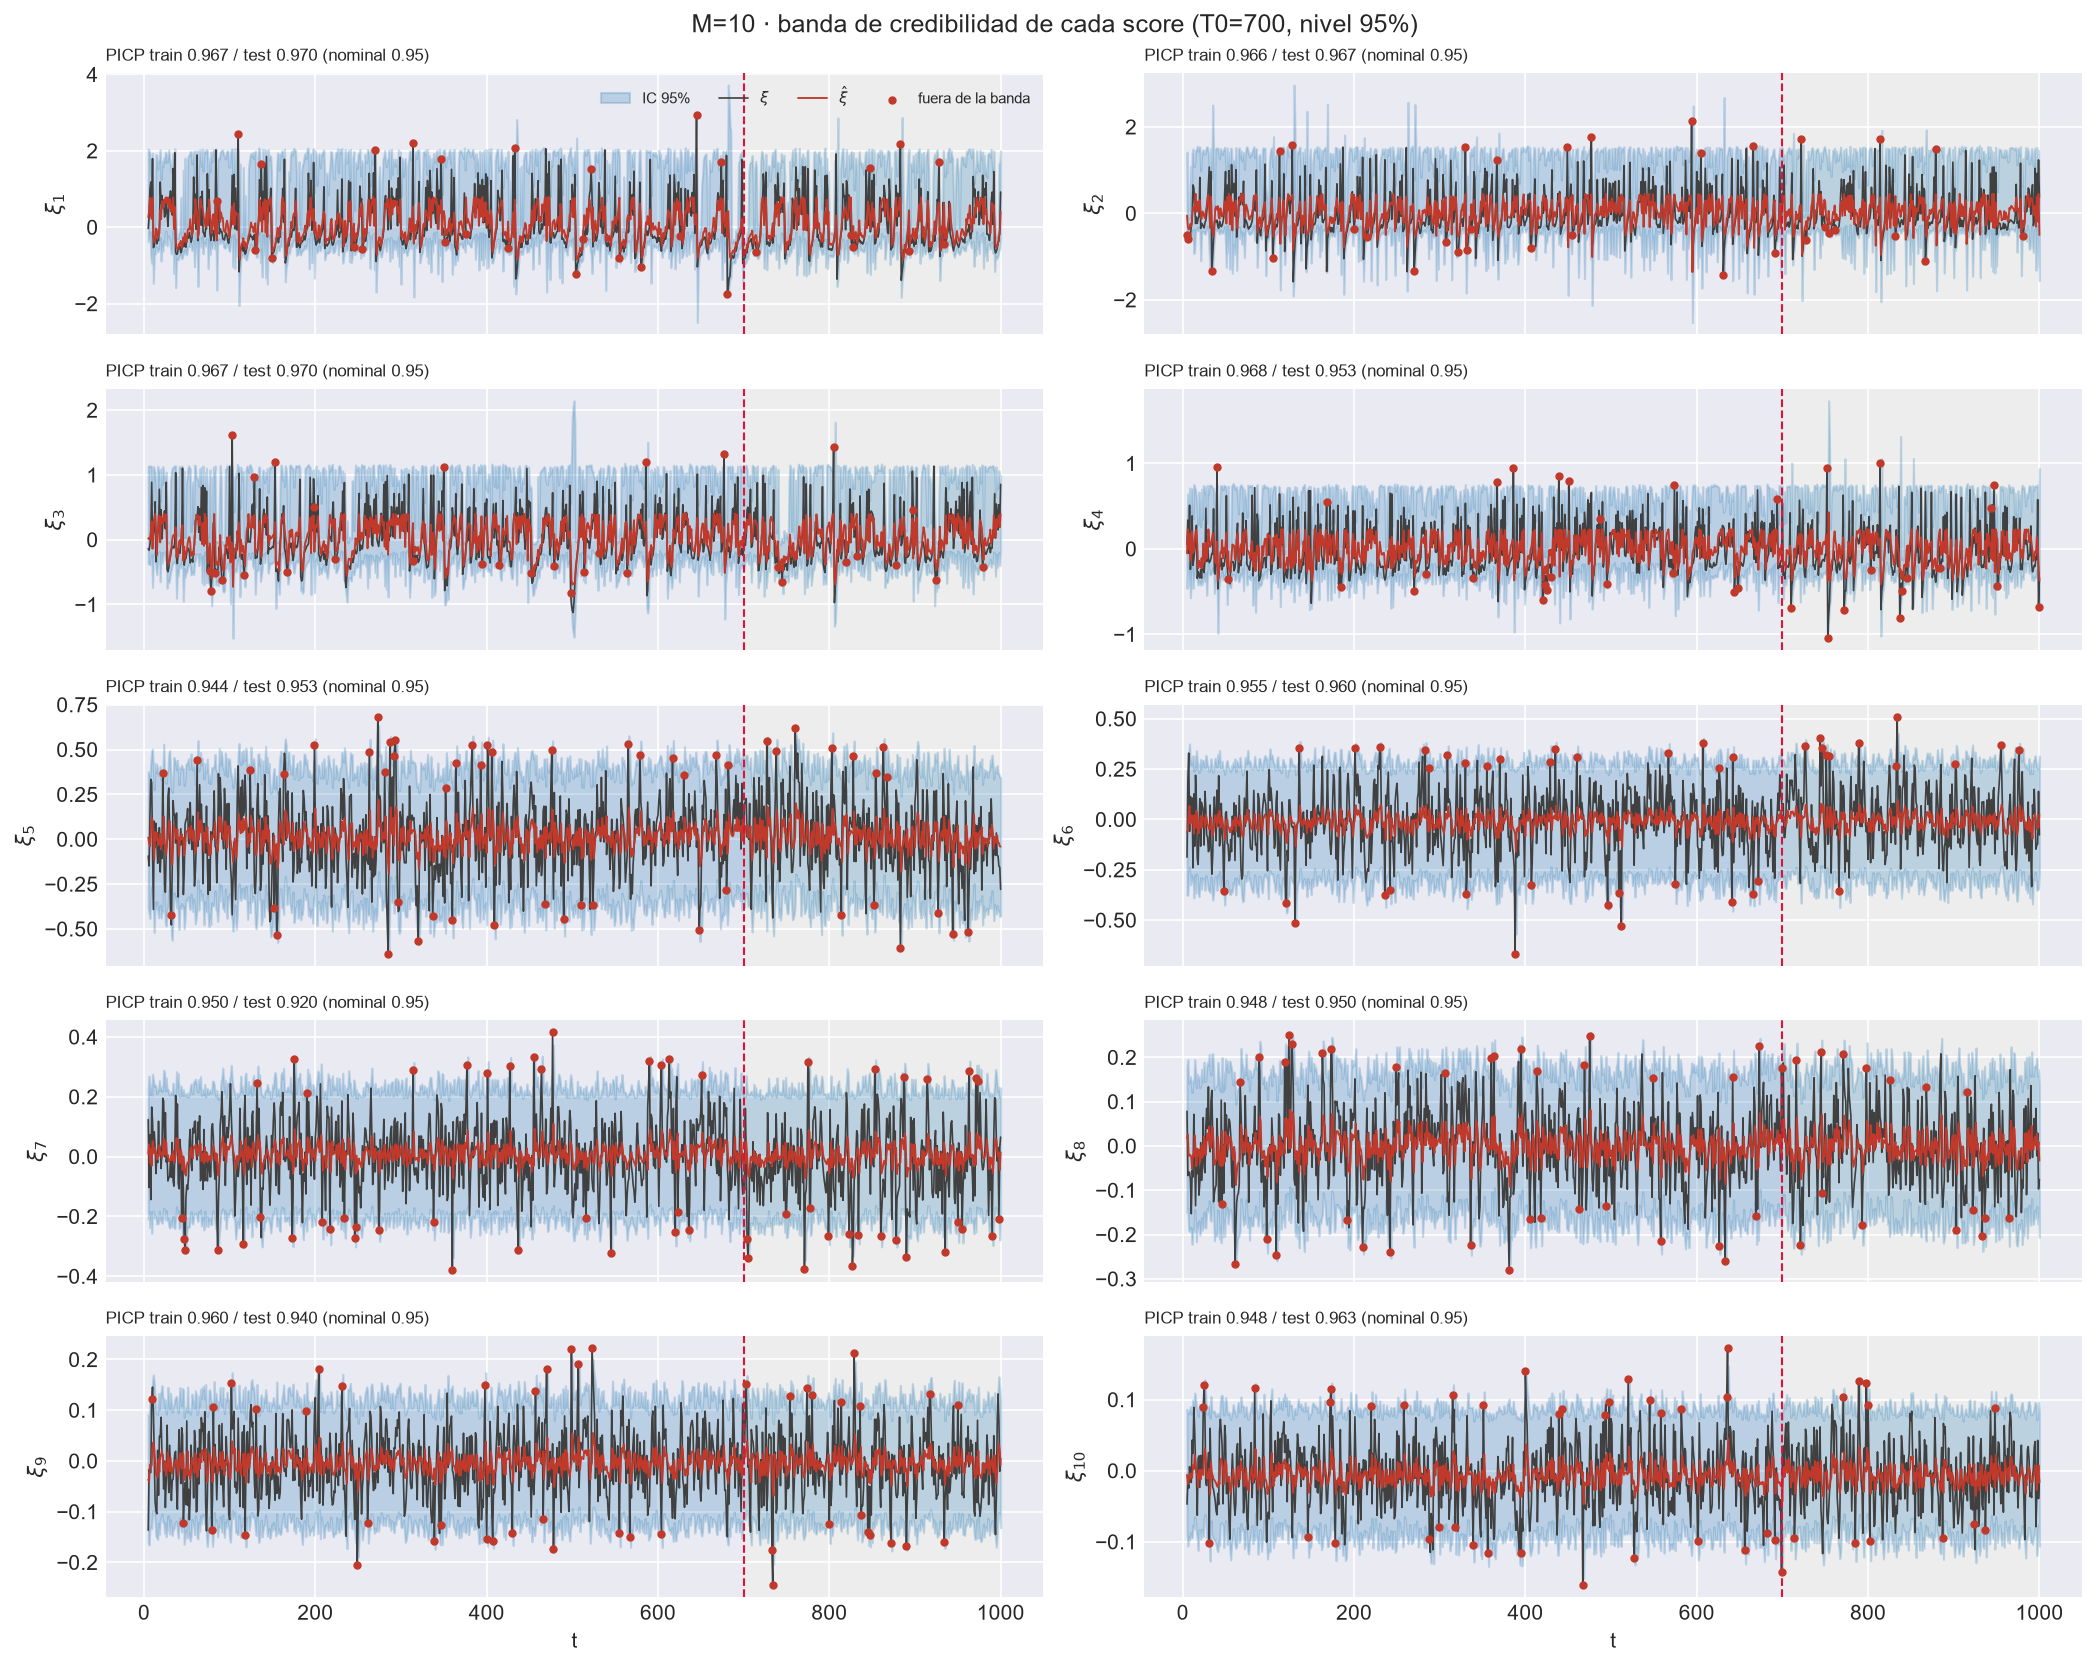
\includegraphics[width=\textwidth,height=0.7\textheight,keepaspectratio]{IMG/aneB_00/aneB_00_scores_banda_C2.png}
\caption{C-2 (TAR). Banda de credibilidad de cada score ($M_{\mathrm{ref}}$).}
\label{fig:aneB_banda_C2}
\end{figure}

\begin{figure}[H]
\centering
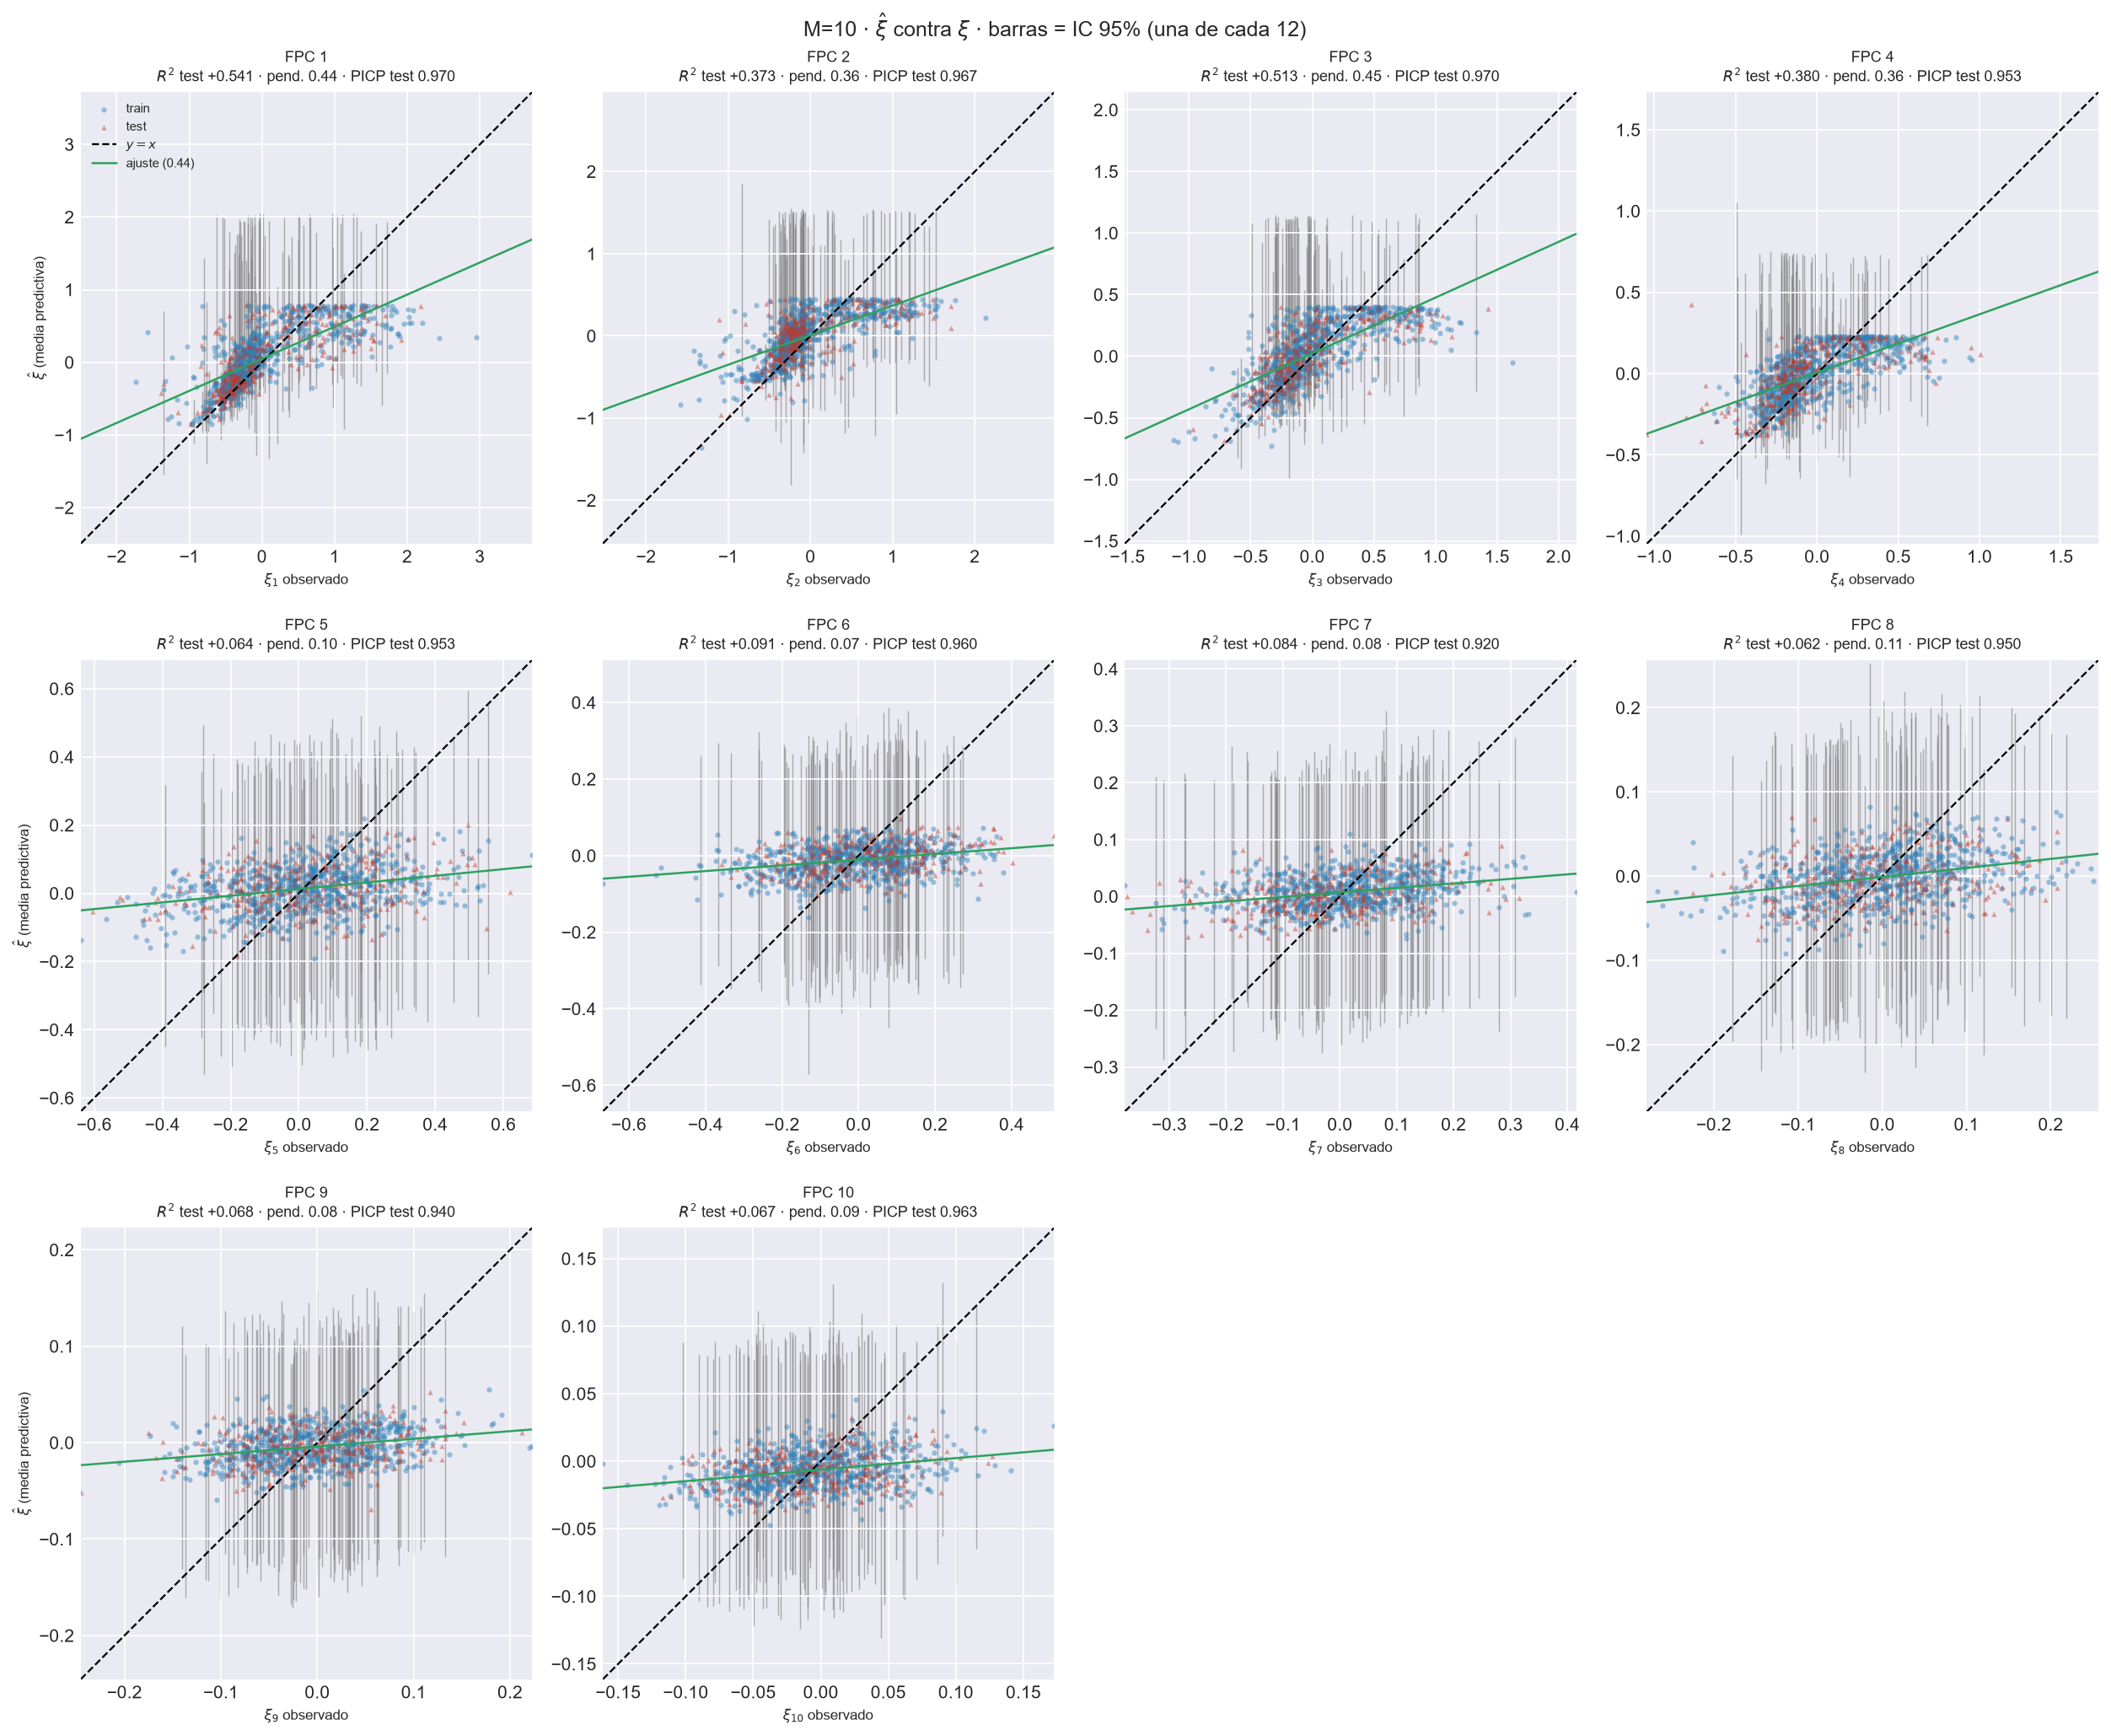
\includegraphics[width=\textwidth,height=0.7\textheight,keepaspectratio]{IMG/aneB_00/aneB_00_scores_dispersion_C2.png}
\caption{C-2 (TAR). Dispersión estimada de cada score frente a la observada ($M_{\mathrm{ref}}$).}
\label{fig:aneB_disp_C2}
\end{figure}

\begin{figure}[H]
\centering
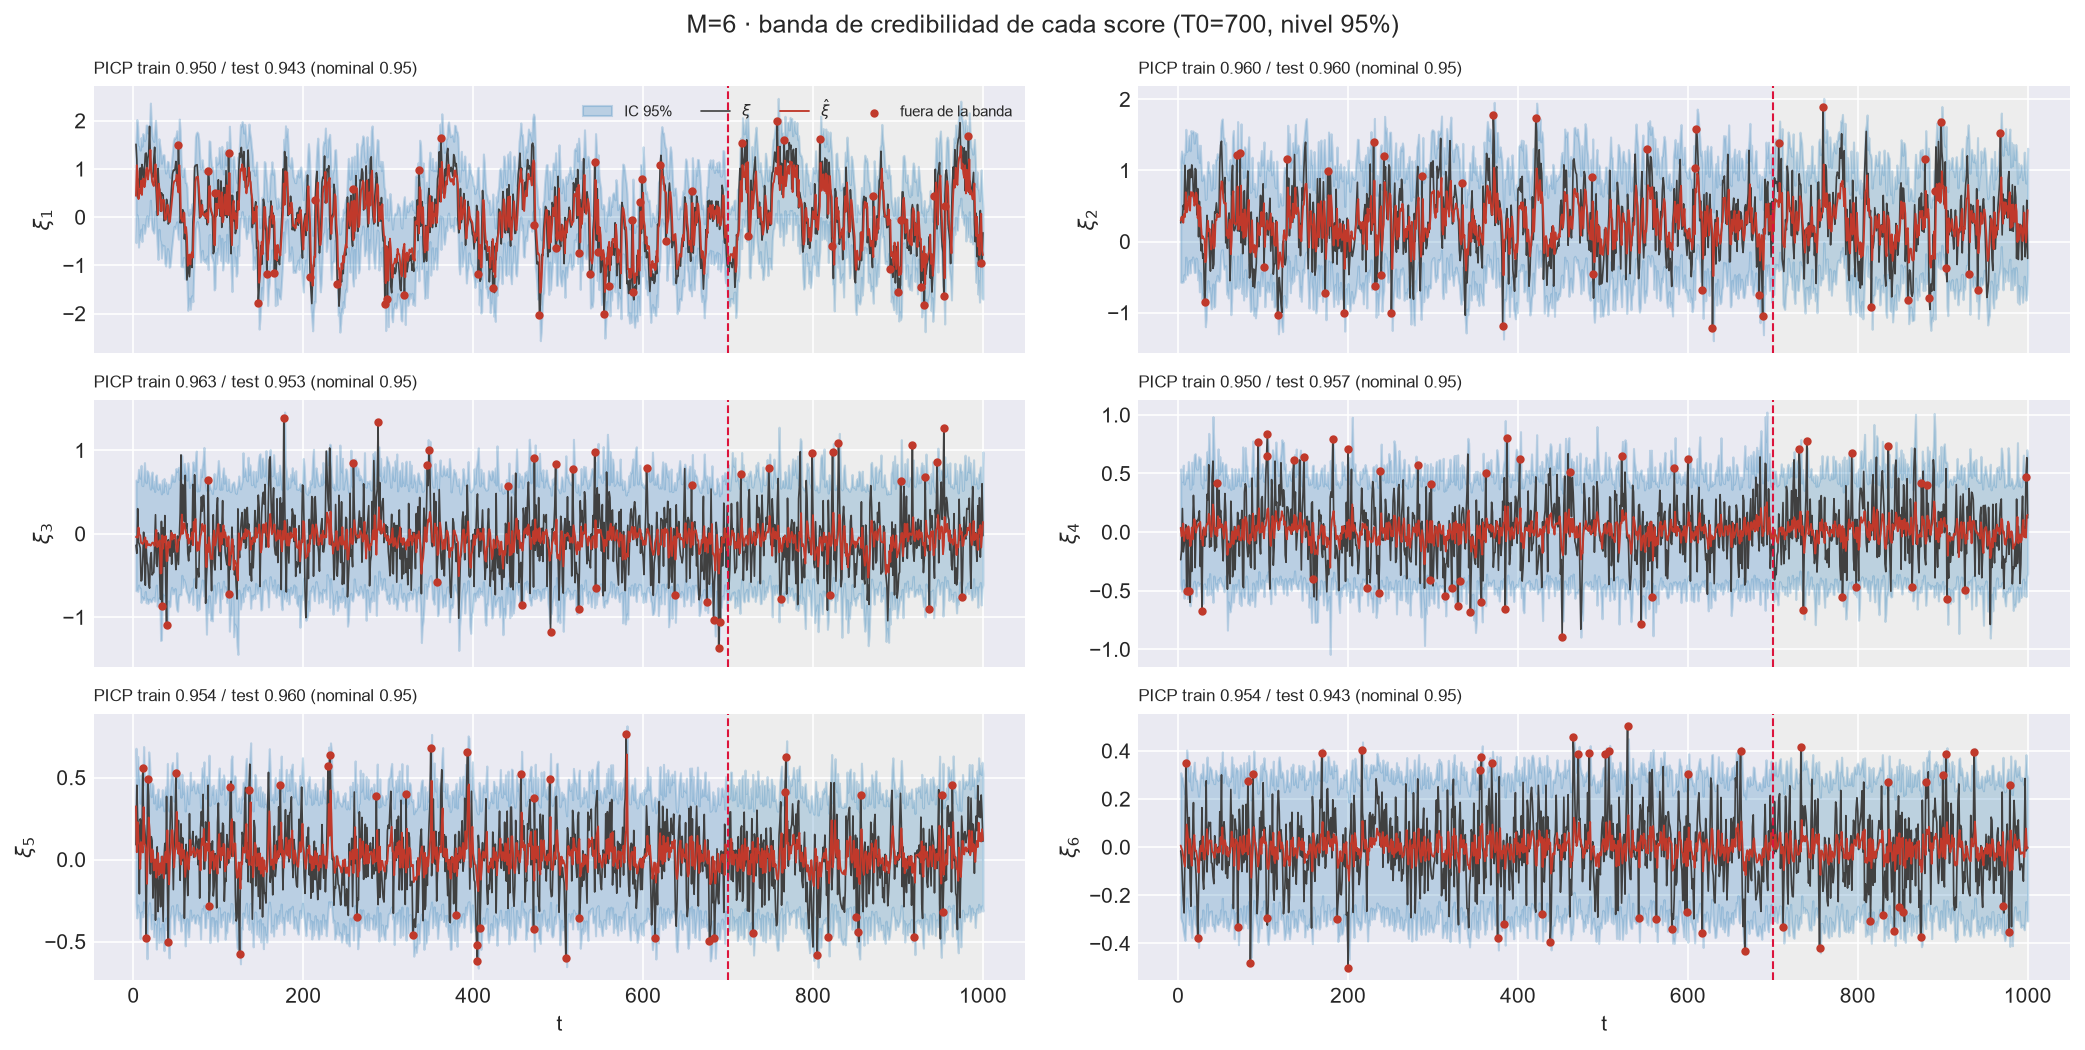
\includegraphics[width=\textwidth,height=0.7\textheight,keepaspectratio]{IMG/aneB_00/aneB_00_scores_banda_C3.png}
\caption{C-3 (multimodalidad). Banda de credibilidad de cada score ($M_{\mathrm{ref}}$).}
\label{fig:aneB_banda_C3}
\end{figure}

\begin{figure}[H]
\centering
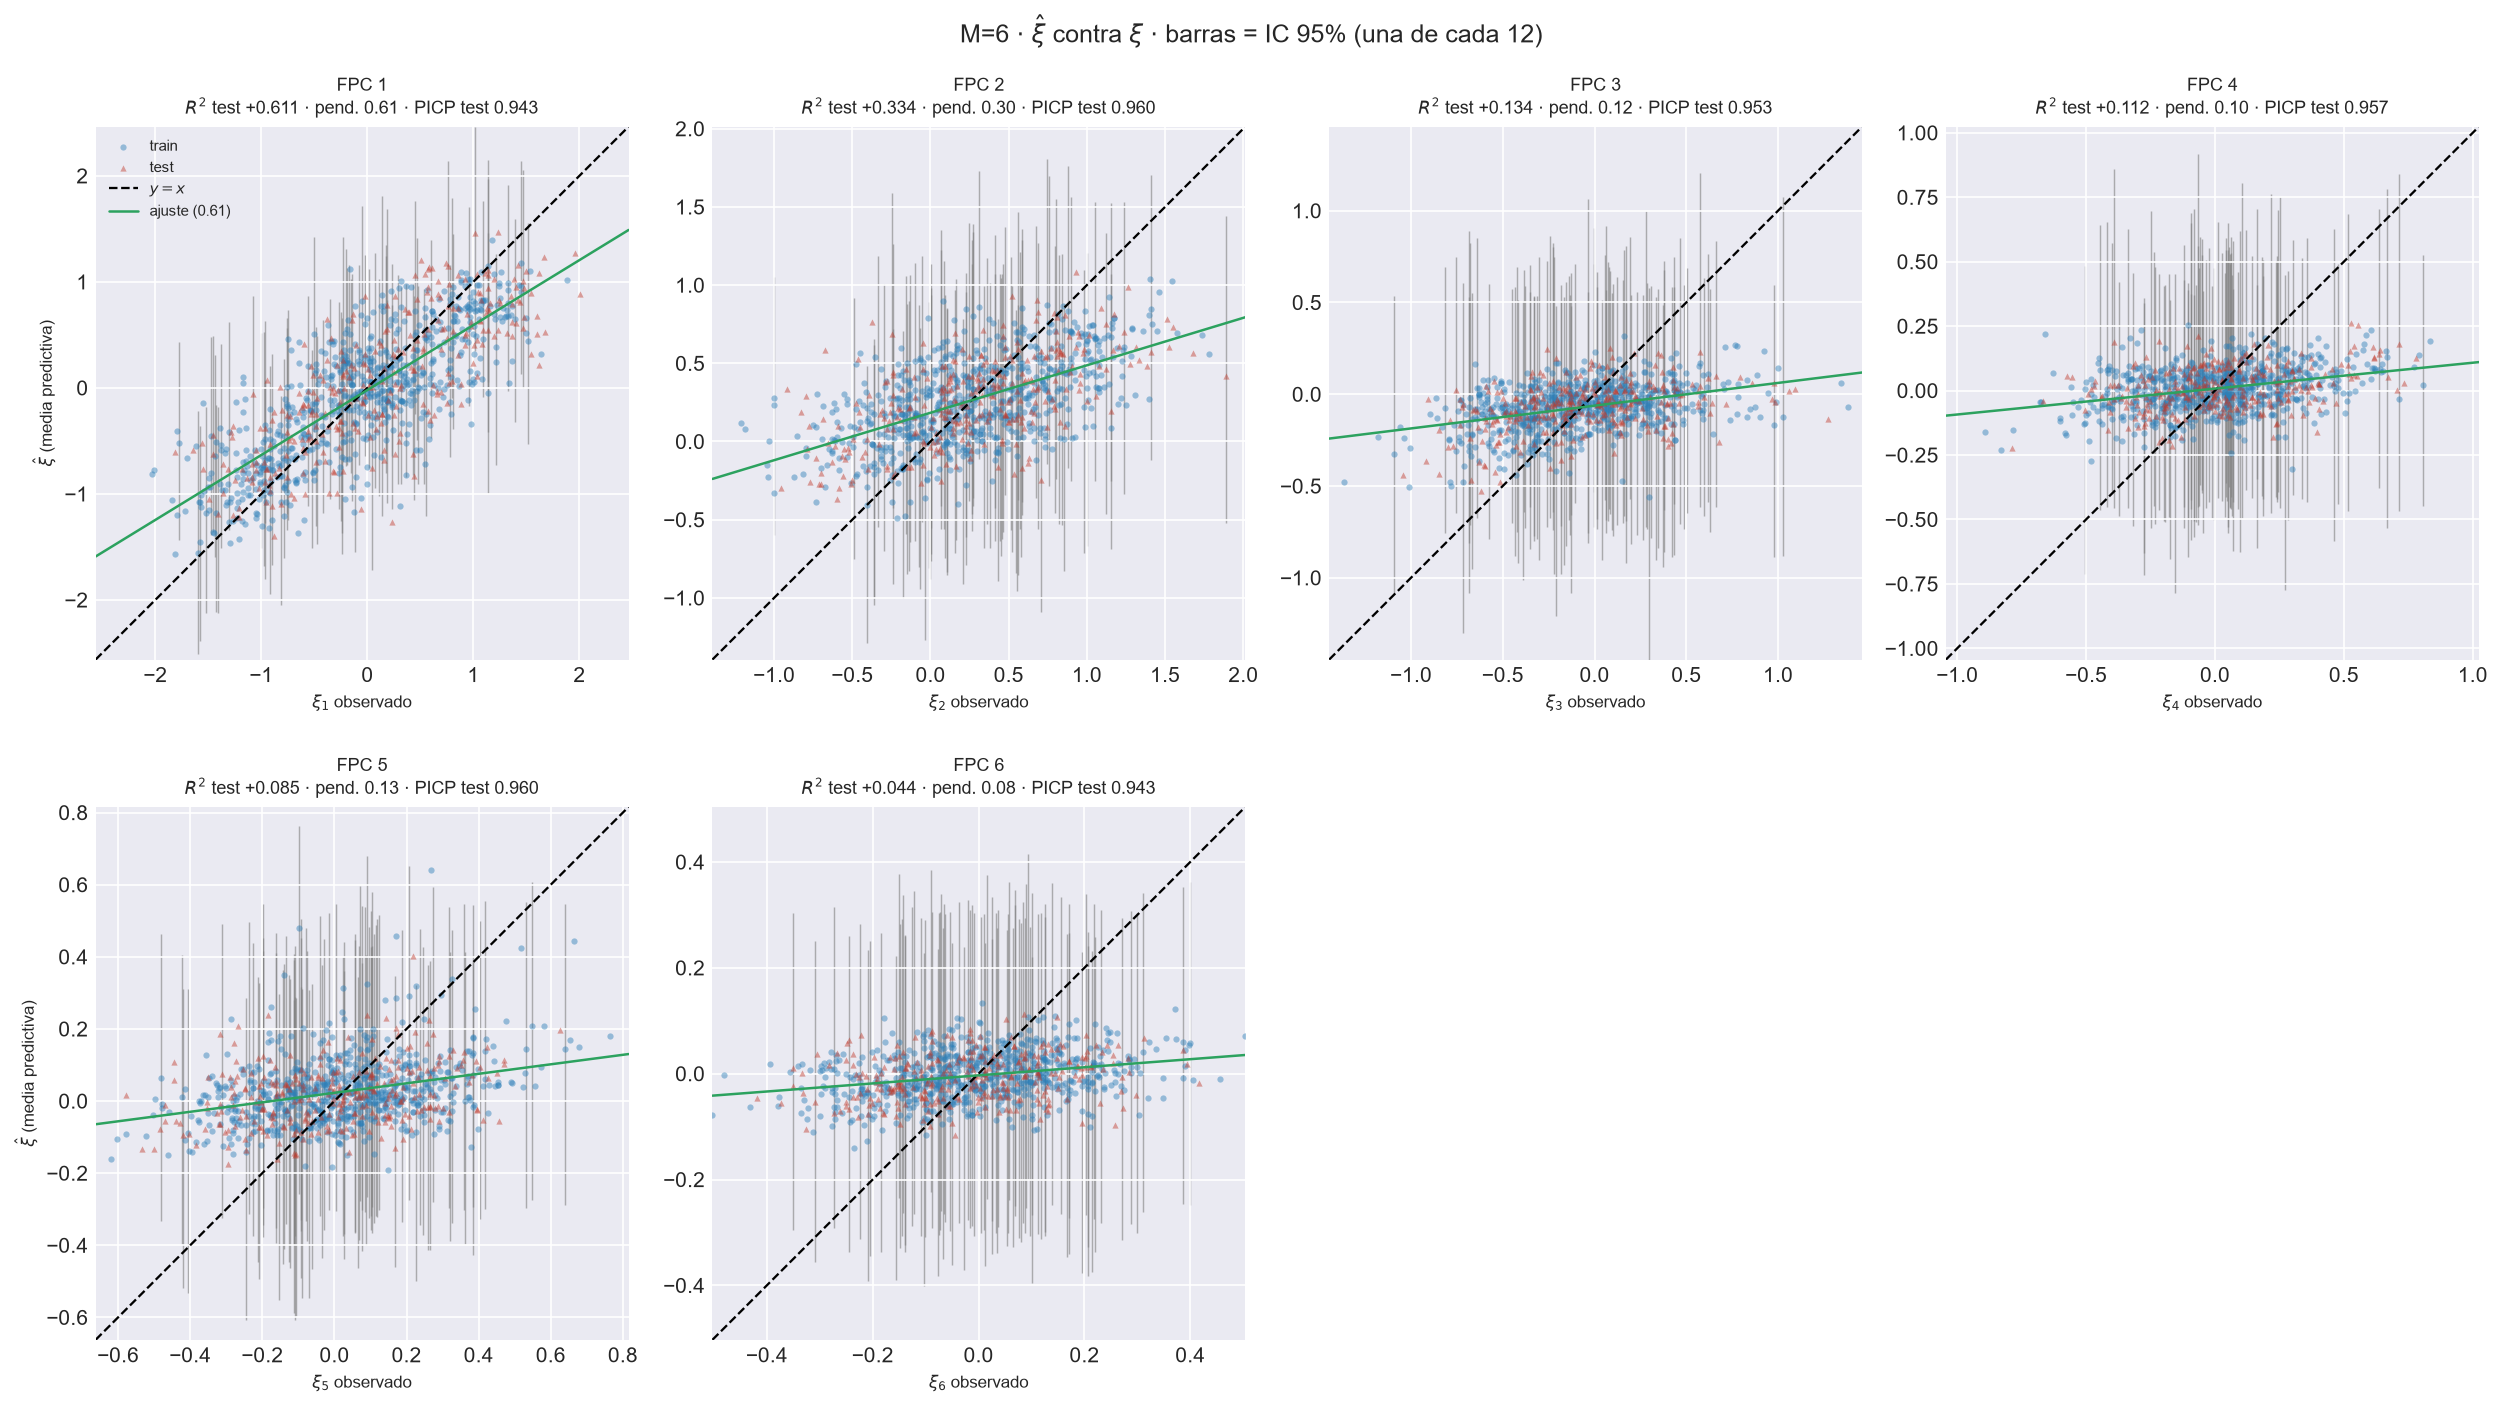
\includegraphics[width=\textwidth,height=0.7\textheight,keepaspectratio]{IMG/aneB_00/aneB_00_scores_dispersion_C3.png}
\caption{C-3 (multimodalidad). Dispersión estimada de cada score frente a la observada ($M_{\mathrm{ref}}$).}
\label{fig:aneB_disp_C3}
\end{figure}

\section{Predicciones curva a curva}
\label{aneB_00_06_predicciones_curvas}

Extractos de predicciones del bloque de prueba y orígenes de mejor y peor desempeño del PSBPM-FD frente al FAR.

\subsection{Escenario C-1 (GARCH)}
\label{aneB_00_06_02_curvas_garch}

\begin{figure}[H]
\centering
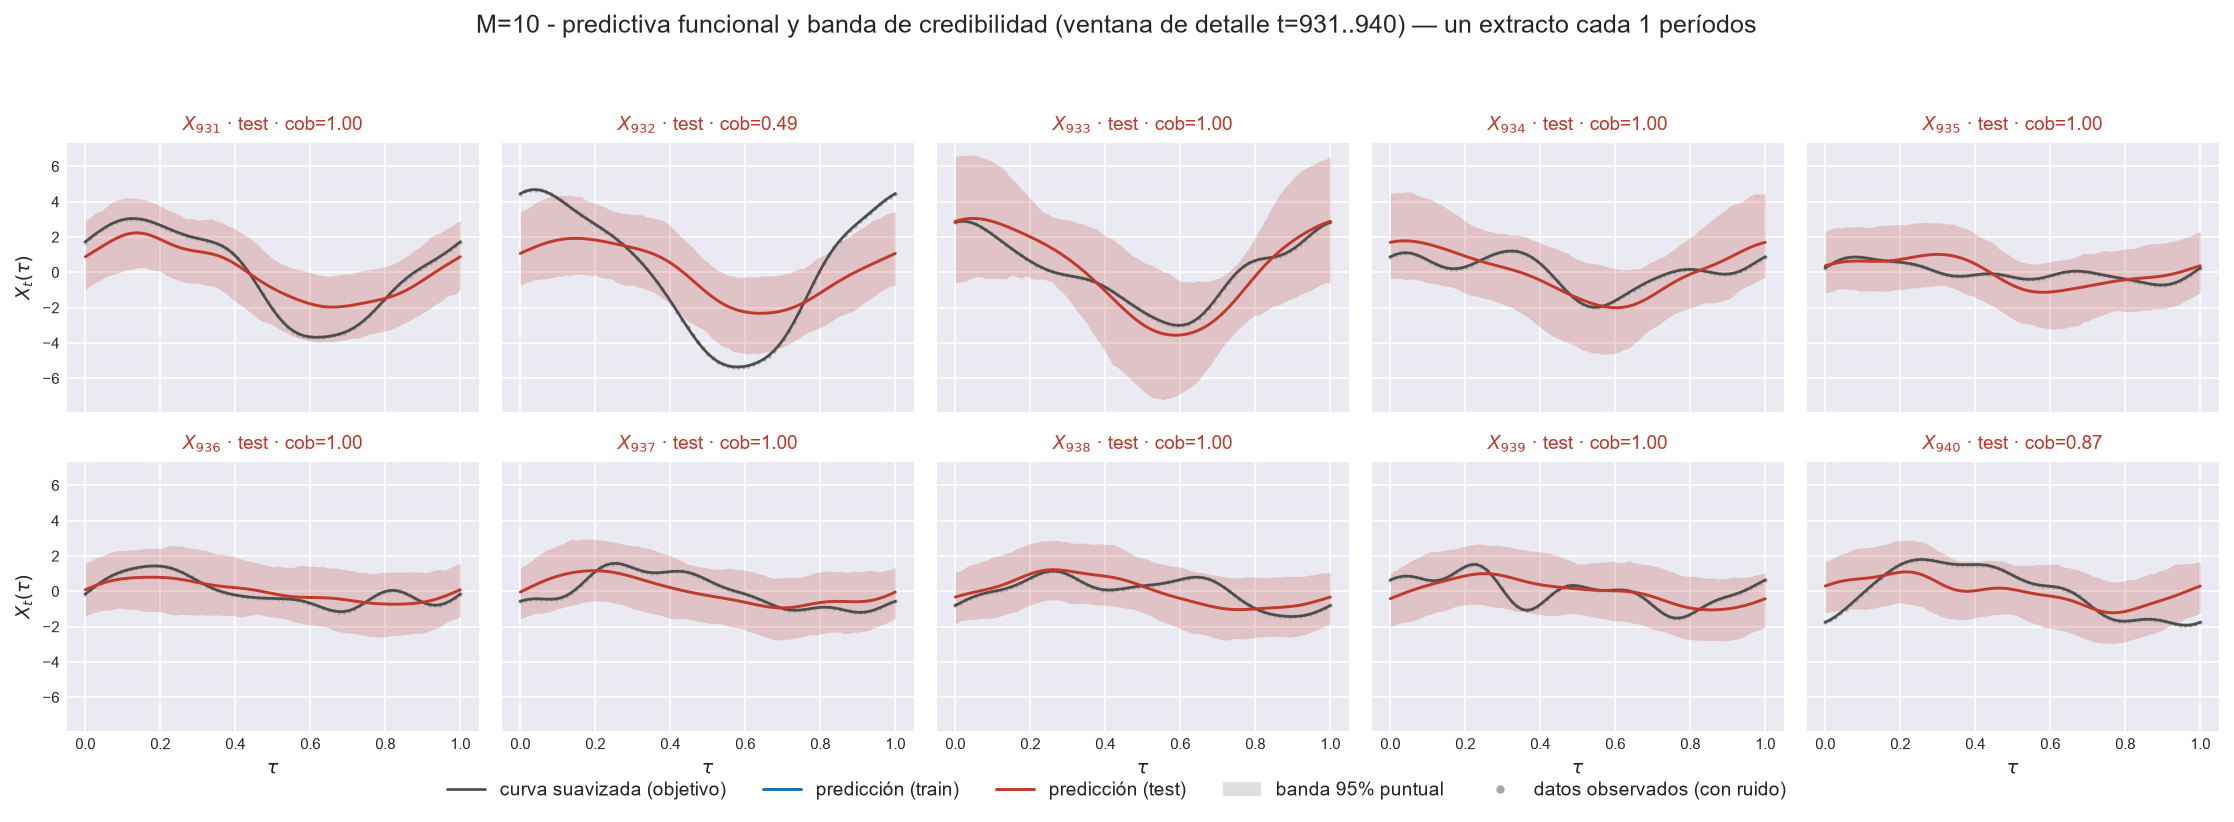
\includegraphics[width=\textwidth,height=0.45\textheight,keepaspectratio]{IMG/aneB_00/aneB_00_curvas_ext_C1.png}
\caption{C-1 (GARCH). Extractos de curvas del bloque de prueba con la predicción y su banda.}
\label{fig:aneB_curvas_ext_C1}
\end{figure}

\begin{figure}[H]
\centering
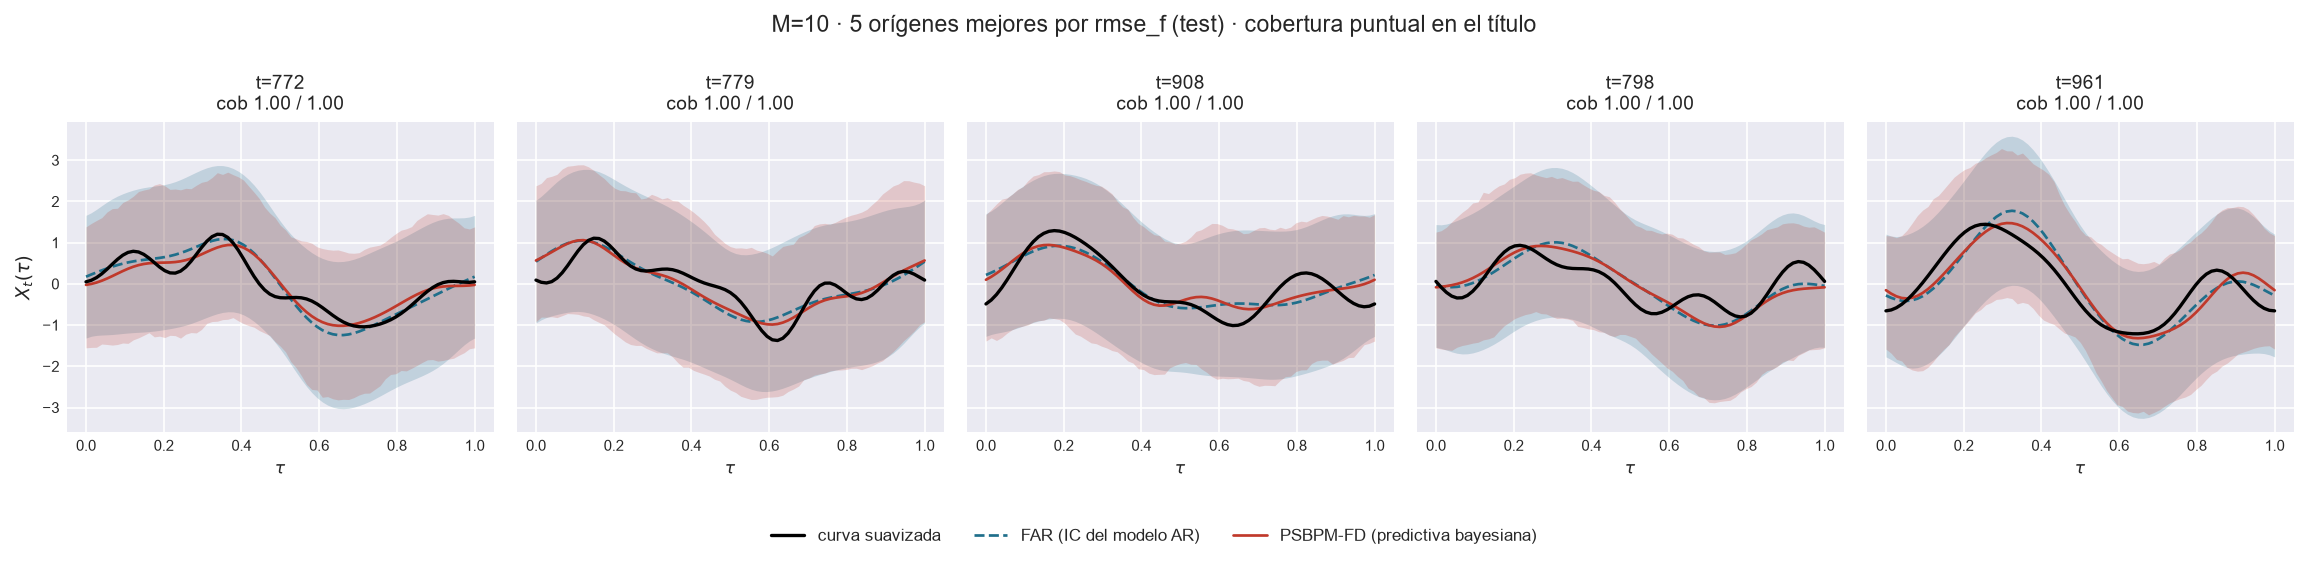
\includegraphics[width=\textwidth,height=0.45\textheight,keepaspectratio]{IMG/aneB_00/aneB_00_curvas_mej_C1.png}
\caption{C-1 (GARCH). Orígenes con mejor desempeño del PSBPM-FD frente al FAR.}
\label{fig:aneB_curvas_mej_C1}
\end{figure}

\begin{figure}[H]
\centering
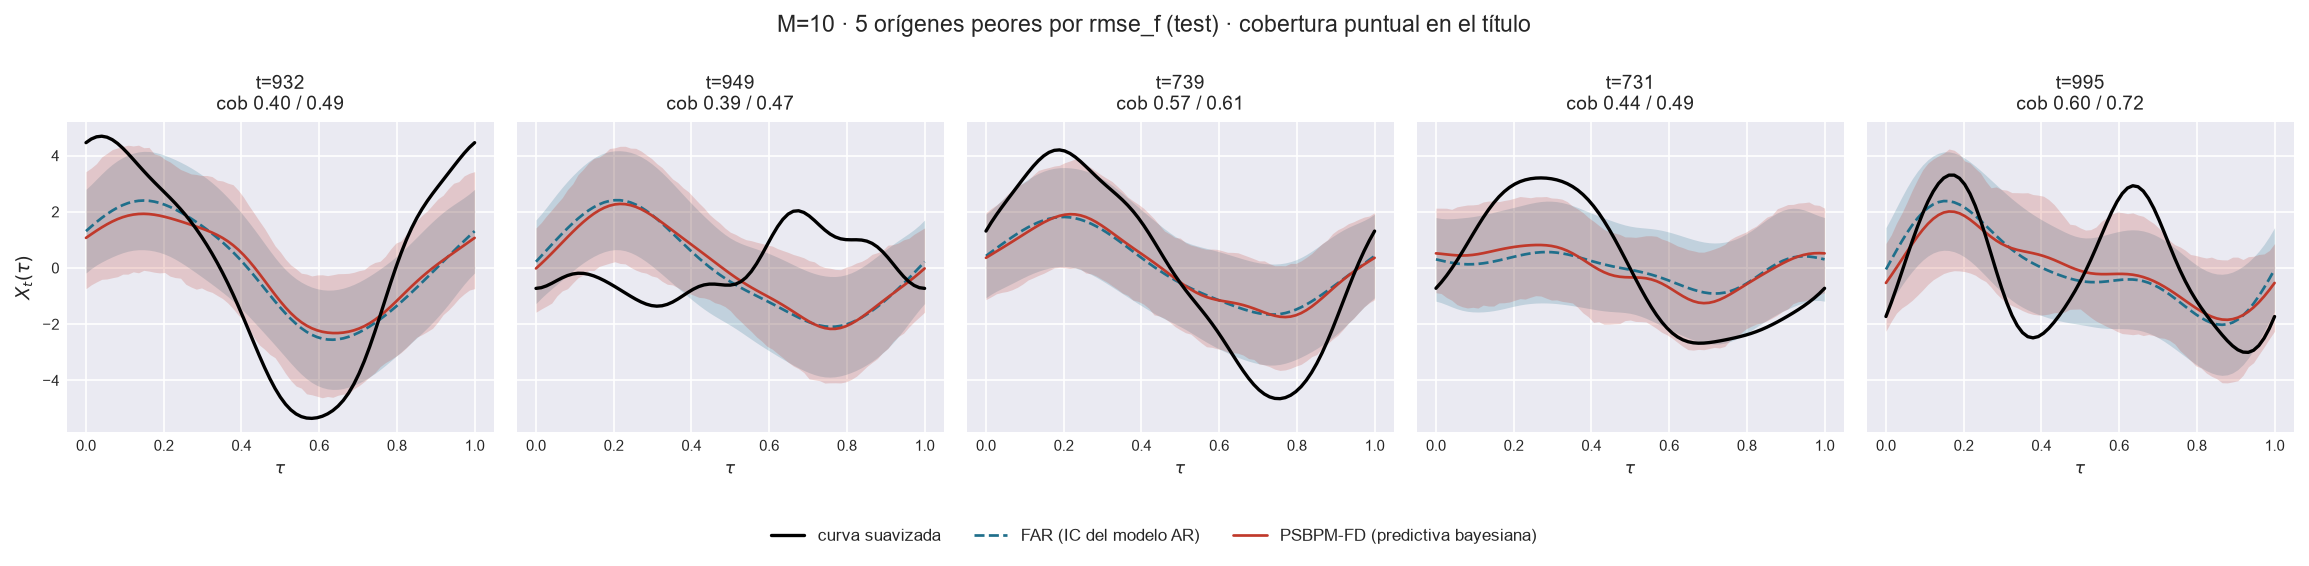
\includegraphics[width=\textwidth,height=0.45\textheight,keepaspectratio]{IMG/aneB_00/aneB_00_curvas_peo_C1.png}
\caption{C-1 (GARCH). Orígenes con peor desempeño del PSBPM-FD frente al FAR.}
\label{fig:aneB_curvas_peo_C1}
\end{figure}

\subsection{Escenario C-2 (TAR)}
\label{aneB_00_06_01_curvas_tar}

\begin{figure}[H]
\centering
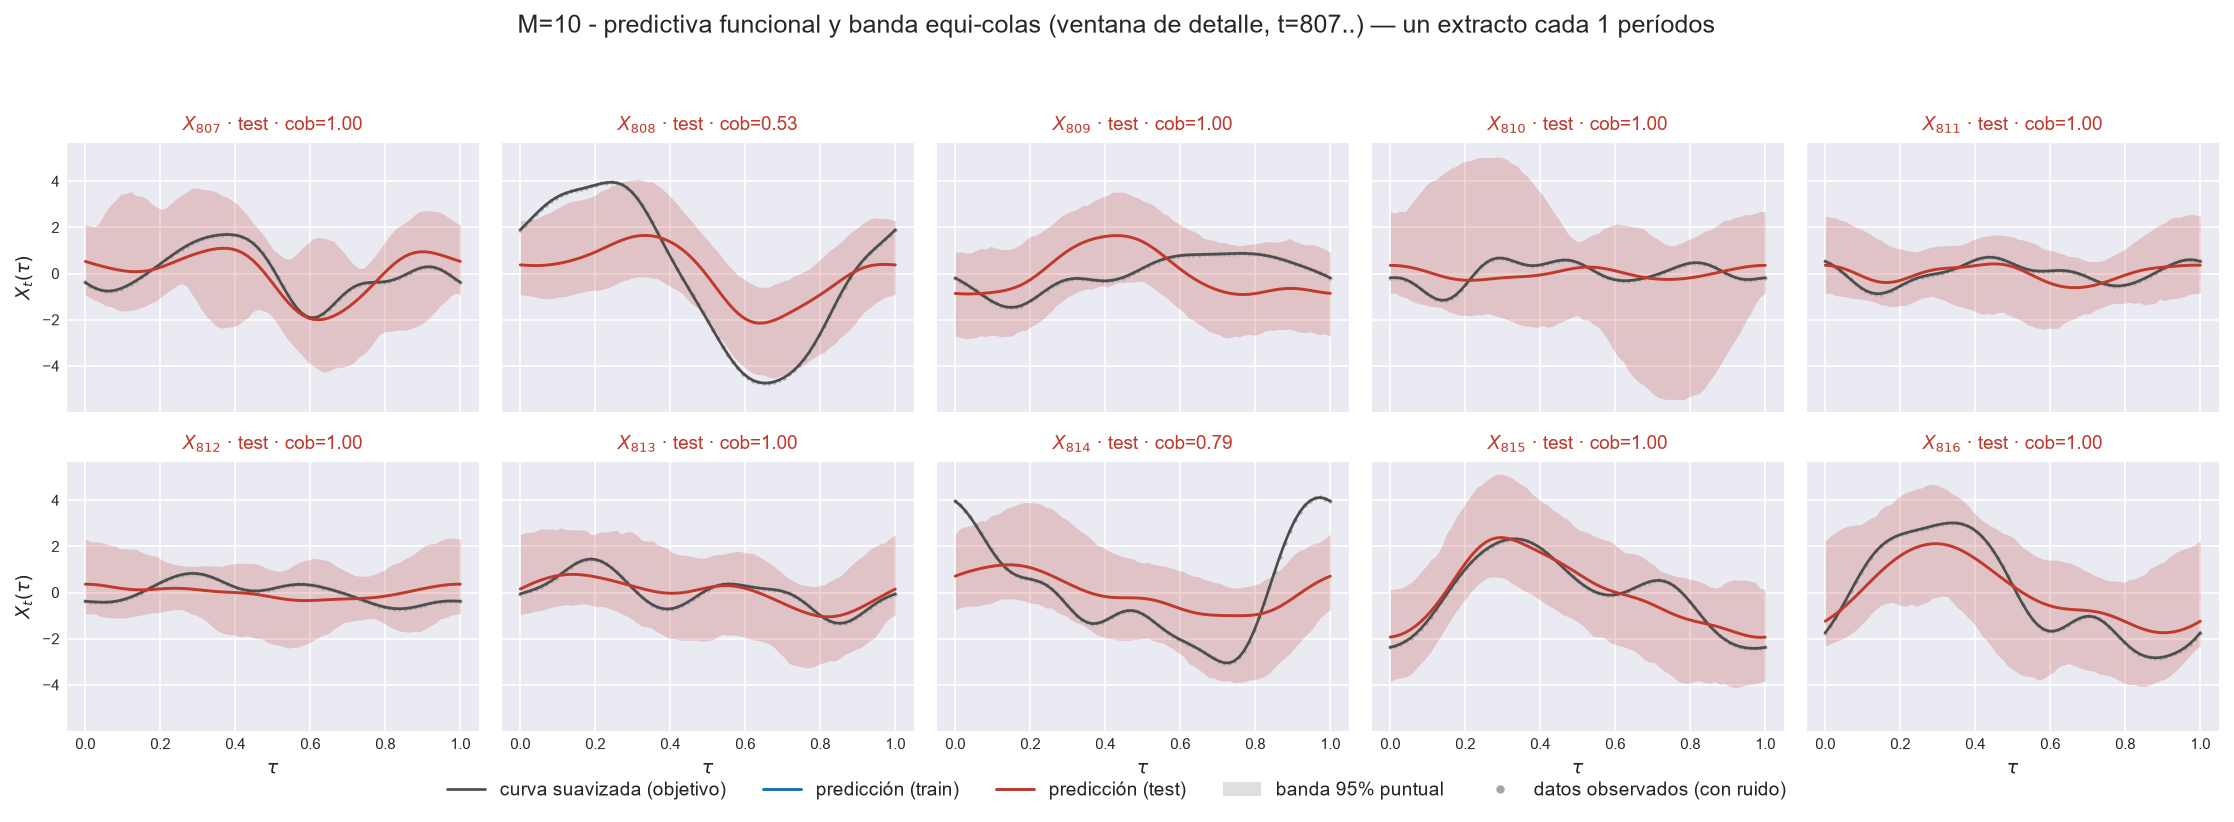
\includegraphics[width=\textwidth,height=0.45\textheight,keepaspectratio]{IMG/aneB_00/aneB_00_curvas_ext_C2.png}
\caption{C-2 (TAR). Extractos de curvas del bloque de prueba con la predicción y su banda.}
\label{fig:aneB_curvas_ext_C2}
\end{figure}

\begin{figure}[H]
\centering
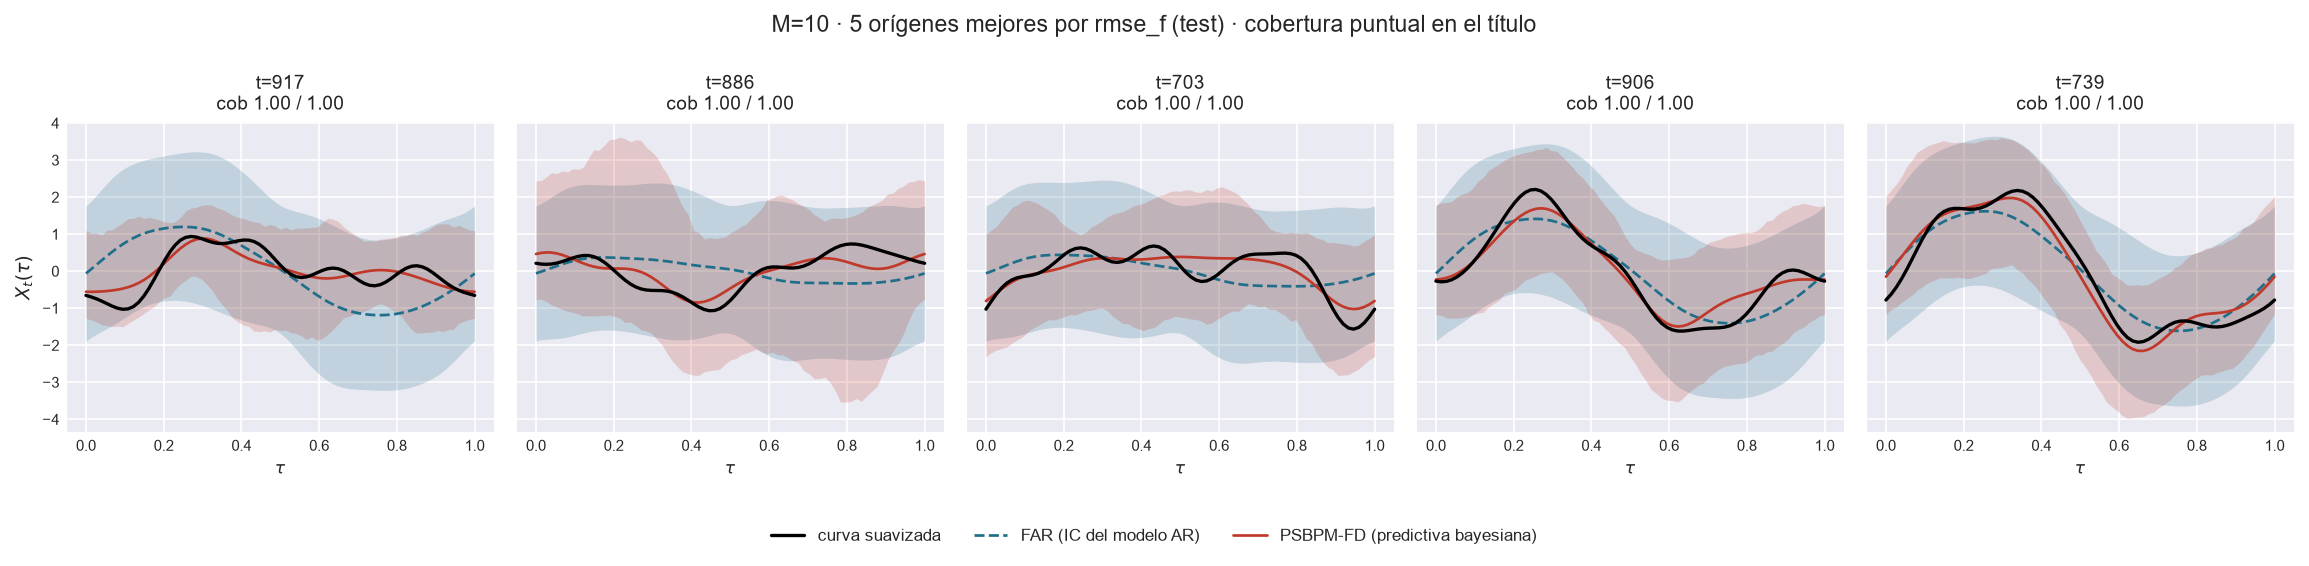
\includegraphics[width=\textwidth,height=0.45\textheight,keepaspectratio]{IMG/aneB_00/aneB_00_curvas_mej_C2.png}
\caption{C-2 (TAR). Orígenes con mejor desempeño del PSBPM-FD frente al FAR.}
\label{fig:aneB_curvas_mej_C2}
\end{figure}

\begin{figure}[H]
\centering
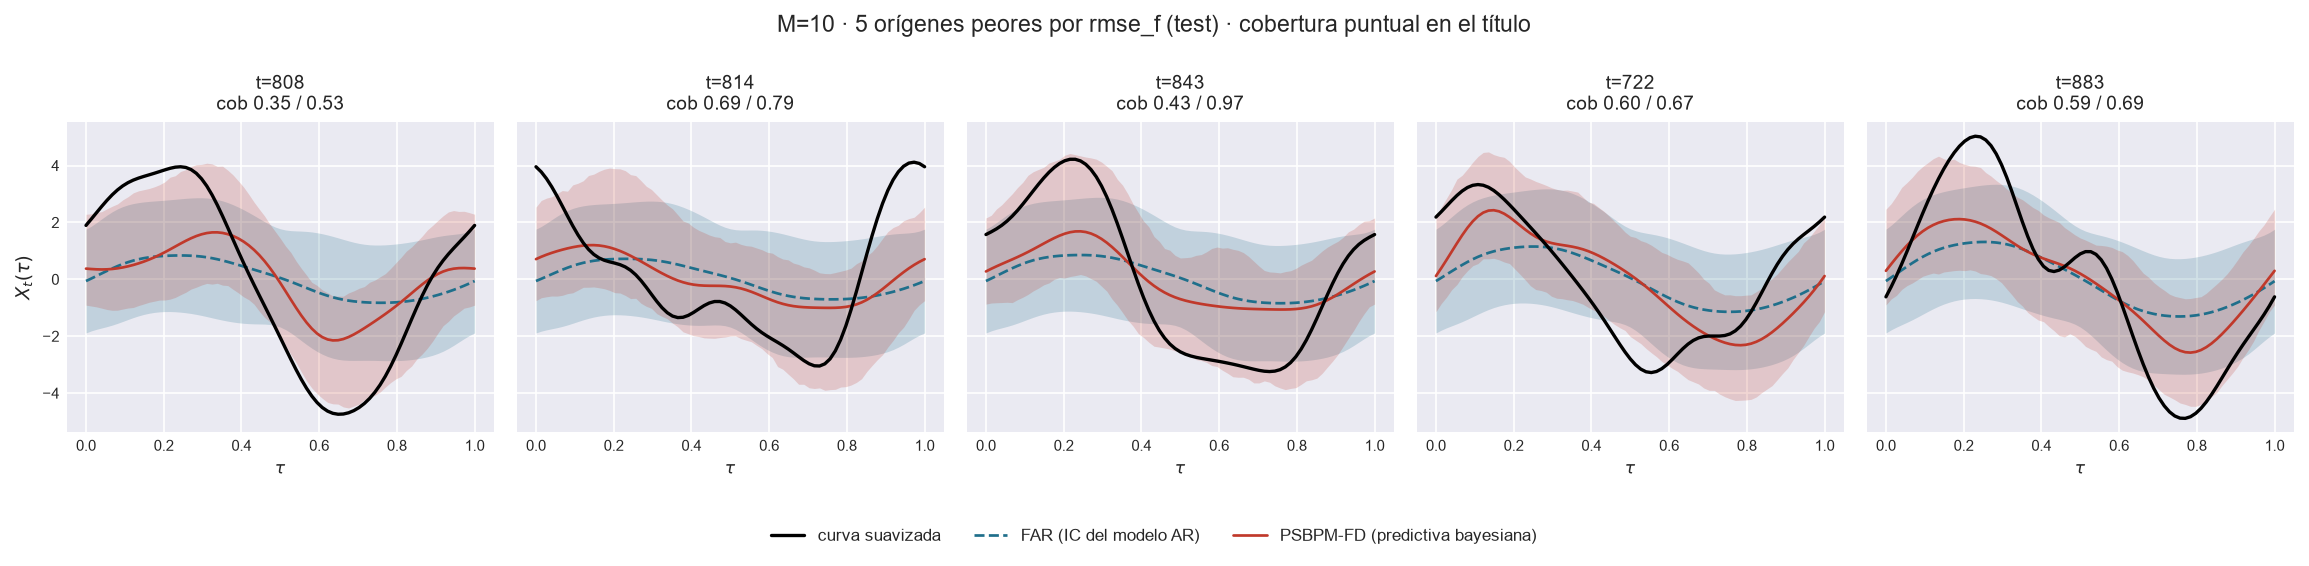
\includegraphics[width=\textwidth,height=0.45\textheight,keepaspectratio]{IMG/aneB_00/aneB_00_curvas_peo_C2.png}
\caption{C-2 (TAR). Orígenes con peor desempeño del PSBPM-FD frente al FAR.}
\label{fig:aneB_curvas_peo_C2}
\end{figure}

\subsection{Escenario C-3 (multimodalidad)}
\label{aneB_00_06_03_curvas_multimodal}

\begin{figure}[H]
\centering
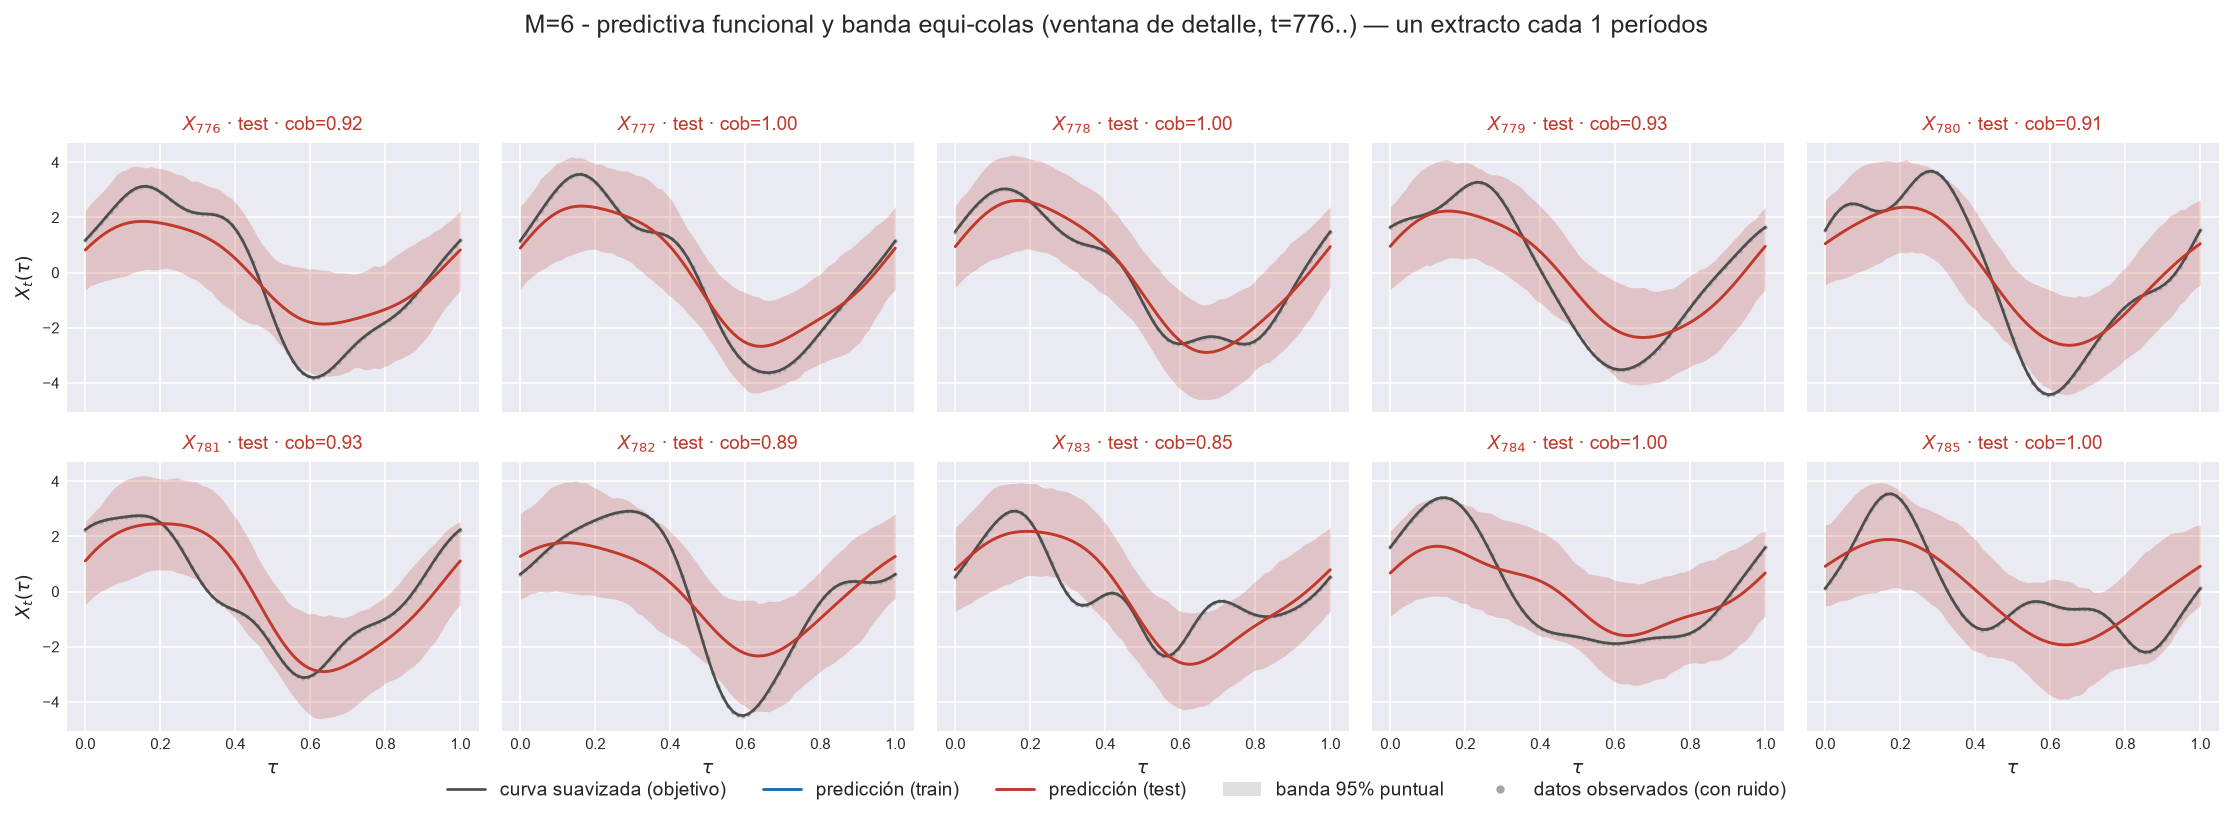
\includegraphics[width=\textwidth,height=0.45\textheight,keepaspectratio]{IMG/aneB_00/aneB_00_curvas_ext_C3.png}
\caption{C-3 (multimodalidad). Extractos de curvas del bloque de prueba con la predicción y su banda.}
\label{fig:aneB_curvas_ext_C3}
\end{figure}

\begin{figure}[H]
\centering
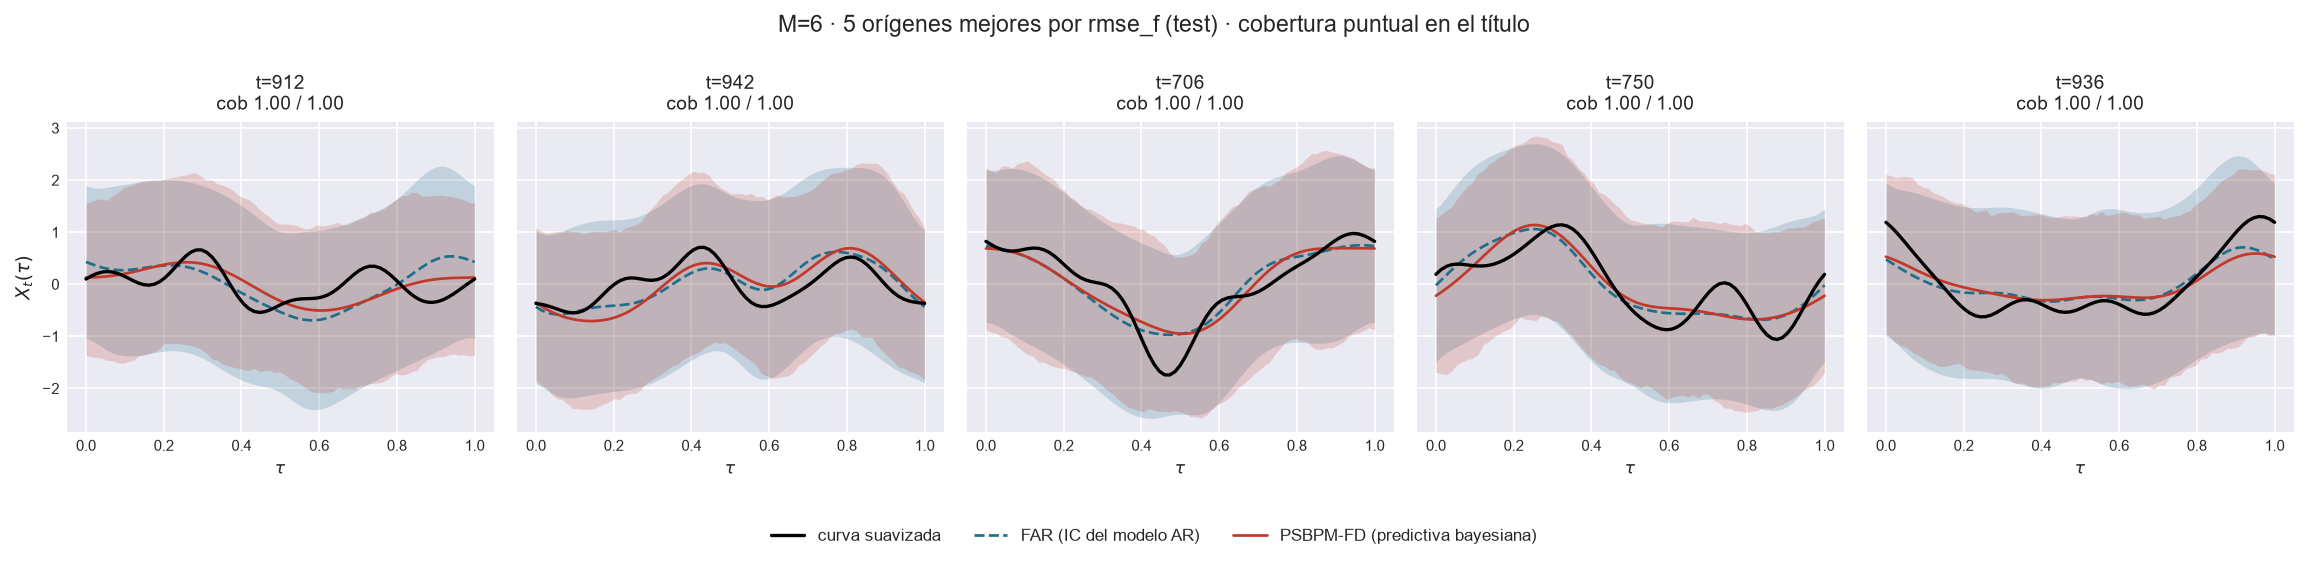
\includegraphics[width=\textwidth,height=0.45\textheight,keepaspectratio]{IMG/aneB_00/aneB_00_curvas_mej_C3.png}
\caption{C-3 (multimodalidad). Orígenes con mejor desempeño del PSBPM-FD frente al FAR.}
\label{fig:aneB_curvas_mej_C3}
\end{figure}

\begin{figure}[H]
\centering
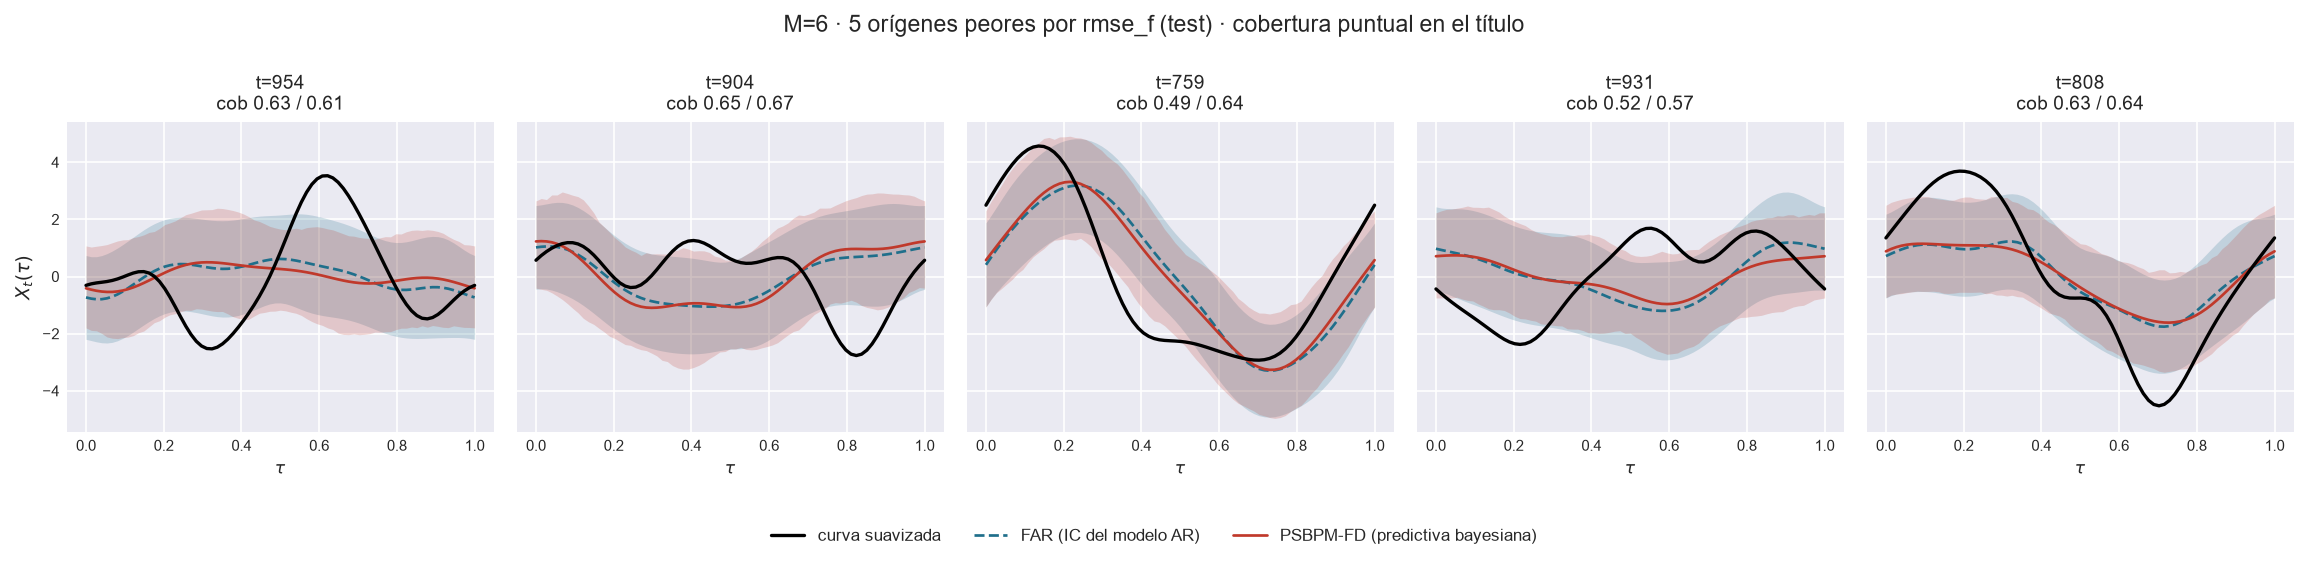
\includegraphics[width=\textwidth,height=0.45\textheight,keepaspectratio]{IMG/aneB_00/aneB_00_curvas_peo_C3.png}
\caption{C-3 (multimodalidad). Orígenes con peor desempeño del PSBPM-FD frente al FAR.}
\label{fig:aneB_curvas_peo_C3}
\end{figure}
